\part*{Part II. Primitive Certification of the Unique Admissible Interior}
\addcontentsline{toc}{part}{Part II. Primitive Certification of the Unique Admissible Interior}

\paragraph{Burden status at entry.}
Part~I has already closed the analytic atlas and shown that no same-scope analytic discriminator closes the wall from inside the classical bundle. Part~II now carries the primitive-side burden: force the unique admissible interior at fixed periodic scope, identify the standard periodic carrier with that interior, and eliminate any rival \emph{standing-positive} same-scope continuation criterion before Part~III begins. The complementary standing-failure branch is not closed here; it is made explicit only after Part~III adds the realized-lineage endpoint-status trichotomy / collapse. What remains after Part~II is therefore not a new analytic estimate but classical realization and faithful transfer of a carrier theorem already fixed locally on the standing-positive branch.

\paragraph{Reader roadmap.} Part~II carries the primitive-side burden of the paper. It does not attempt a new analytic estimate on vortex stretching. Instead it turns the analytic obstruction of Part~I into a fixed-scope admissibility problem on the standard periodic carrier and organizes the manuscript around the claim that, at the fixed periodic scope, this carrier is the \emph{unique admissible interior}. Before the carrier-specific specialization begins, Section~\ref{sec:primitive-base} now begins the structural theorem packet P1--P4, with P1--P4 all proved in this manuscript (the P4 proof core appearing in Appendix~A), and then records a compact fixed-scope necessity chain: no standing-preserving repair, bivalent fail-closed admissibility, no parameterized admissibility crossing, admissible initial conditions are not variables, no admissible variation, and the theorem of the \emph{unique admissible interior}. The theorem-visible bridge packet in Section~\ref{subsec:bridge-packet-periodic} then proves in-paper that the fixed periodic problem instantiates those antecedents and therefore admits the explicit periodic corollary of a unique admissible interior. Section~13.2E then records the carrier-identification packet 13I--13K: the standard carrier realizes that unique admissible interior, no rival same-scope continuation regime survives, and no additional PDE-side continuation criterion remains inside fixed scope. The point of that ordering is claim-type clarity: the primitive layer is made theorem-visible before any reader can mistake Part~II for a hidden same-scope PDE continuation patch or honestly claim that a further same-scope PDE ingredient has been left unstated.
First, the Part~I atlas is closed into a finite gate classification for same-scope continuation mechanisms.
Second, the periodic Navier--Stokes carrier itself forces a minimal specialized rule package: no competing same-scope continuation gates, binary continuation status, no parameterized same-scope gate, and no repair / no generator in specialized NS form. Subsection~13.1A makes this forcing explicit in ordinary Navier--Stokes language.
Third, every \emph{standing-positive} continuation-relevant same-scope candidate determination on the live route is forced through the finite typed decision packet 13.5E--13.5L, showing branch by branch that no independent standing-positive same-scope continuation discriminator survives on the standard carrier.
Fourth, only after that finite classification and elimination packet is on the page do zero-parameter certification together with the narrowed continuation-completeness package verify the standing-positive carrier-side completeness claim actually used on the live proof chain, and Theorem~\ref{thm:ns-carrier-verifies-rule-package} verifies the Part~II rule packet for this specific periodic carrier in that theorem-local sense. Subsection~13.2A records the explicit translation dictionary used on that standing-positive route, and Section~13.2D interprets the derived carrier-specific exhaustion theorem as a same-scope existence statement on the fixed carrier. The completeness claims in these subsections are therefore frozen at the domain they visibly prove rather than silently enlarged to full same-scope totality before the later endgame hardening work.
Fifth, structural regularity and branch elimination force regularity on the carrier already identified with the unique admissible interior, and the terminality package shows in Clay-facing form that no same-scope analytic escape remains for the official periodic problem.

\begin{figure}[p]
\centering
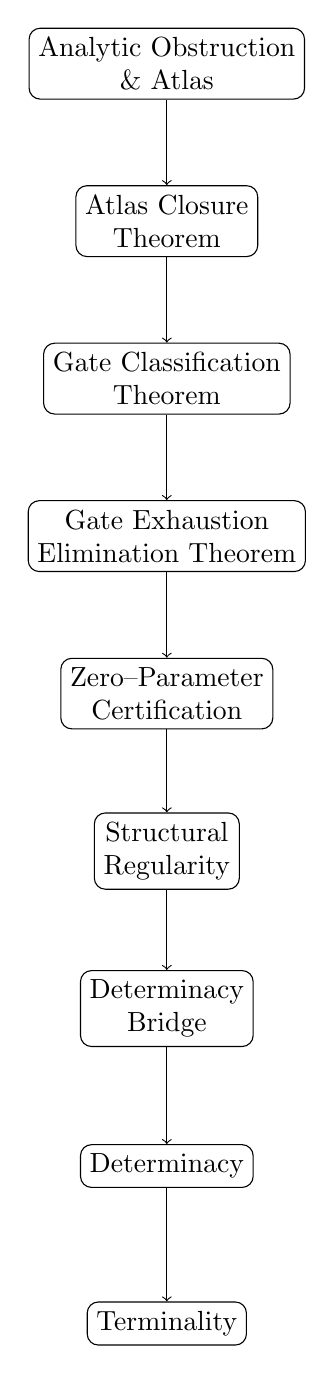
\begin{tikzpicture}[node distance=2cm, every node/.style={draw, rectangle, rounded corners, align=center}]
\node (atlas) {Analytic Obstruction\\\& Atlas};
\node (closure) [below of=atlas] {Atlas Closure\\Theorem};
\node (class) [below of=closure] {Gate Classification\\Theorem};
\node (exhaust) [below of=class] {Gate Exhaustion\\Elimination Theorem};
\node (cert) [below of=exhaust] {Zero--Parameter\\Certification};
\node (reg) [below of=cert] {Structural\\Regularity};
\node (detb) [below of=reg] {Determinacy\\Bridge};
\node (det) [below of=detb] {Determinacy};
\node (term) [below of=det] {Terminality};

\draw[->] (atlas) -- (closure);
\draw[->] (closure) -- (class);
\draw[->] (class) -- (exhaust);
\draw[->] (exhaust) -- (cert);
\draw[->] (cert) -- (reg);
\draw[->] (reg) -- (detb);
\draw[->] (detb) -- (det);
\draw[->] (det) -- (term);
\end{tikzpicture}
\caption{Dependency diagram for the carrier-side segment of the Navier--Stokes admissibility cascade. The fixed-scope primitive necessity layer is proved in Section~\ref{sec:primitive-base} and feeds the cascade shown here.}
\end{figure}

\begin{tcolorbox}[title=Navier--Stokes admissibility cascade]
The structural resolution proceeds through the following theorem cascade:

\begin{enumerate}[leftmargin=2.2em]
\item Analytic Obstruction Theorem (\Cref{thm:analytic-obstruction})
\item Atlas Closure Theorem (\Cref{thm:atlas-closure})
\item Gate Classification Theorem (\Cref{thm:gate-classification})
\item Primitive necessity at fixed scope (\Cref{lem:no-standing-preserving-repair}, \Cref{prop:fixed-scope-bivalence}, \Cref{lem:no-parameterized-admissibility-crossing}, \Cref{lem:admissible-initial-conditions-not-variables}, \Cref{lem:no-admissible-variation-fixed-scope}, \Cref{thm:unique-admissible-interior-fixed-scope})
\item Specialized no-second-gate theorem package (\Cref{thm:ns-no-competing-gates}, \Cref{cor:ns-binary-continuation-status}, \Cref{cor:ns-no-parameterized-gate}, \Cref{thm:ns-no-repair-generator})
\item 13.5A--D: the periodic carrier forces the minimal rule package
\item Finite standing-positive same-scope decision packet (13.5E--13.5L, especially Theorem~\ref{thm:13-5F-finite-same-scope-classification} and Corollary~\ref{cor:13-5L-rival-elimination})
\item Gate Exhaustion Elimination Theorem (\Cref{thm:gate-exhaustion})
\item Zero--Parameter Certification (\Cref{thm:ns-zero-parameter})
\item Standing-positive scope-completeness theorem for the standard carrier (\Cref{thm:scope-completeness-standard-carrier})
\item Architectural standing-positive continuation-completeness of the standard carrier (\Cref{thm:strong-continuation-completeness-standard-carrier})
\item Verification of the Part~II rule package for the standard periodic carrier (\Cref{thm:ns-carrier-verifies-rule-package})
\item Structural Regularity Theorem (\Cref{thm:structural-closure})
\item Determinacy Bridge Lemma (\Cref{lem:determinacy-bridge})
\item Determinacy Corollary (\Cref{cor:determinacy-forced})
\item Terminality Theorem (\Cref{thm:terminality})
\item No same-scope analytic escape for the official periodic problem (\Cref{cor:no-same-scope-analytic-escape})
\end{enumerate}

\[
\begin{aligned}
\text{analytic atlas}
&\rightarrow \text{gate classification}
\rightarrow \text{primitive necessity}\\
&\rightarrow \text{minimal rule package}
\rightarrow \text{finite standing-positive same-scope classification}\\
&\rightarrow \text{gate exhaustion}
\rightarrow \text{zero-parameter certification}\\
&\rightarrow \text{standing-positive scope completeness}
\rightarrow \text{architectural continuation-completeness}\\
&\rightarrow \text{rule-package verification}
\rightarrow \text{structural regularity}.
\end{aligned}
\]
\end{tcolorbox}


\section{Primitive necessity at fixed scope, the unique admissible interior, and the Part II rule package}\label{sec:primitive-base}
\paragraph{Burden status.}
At this section entry the analytic burden has already been discharged by Part~I. The remaining task is to prove, inside the manuscript and at fixed scope, that admissibility is bivalent, non-parameterized, and uniqueness-forcing, then transport that fixed-scope packet into the periodic specialization. Nothing in this section appeals to Part~III or to any hidden classical continuation principle.
Part~II is now theorem-explicit about its primitive dependencies. Tier~A now begins the structural theorem packet P1--P4: all four theorems are proved in-paper, with P4 routed through the minimal appendix gate/exhaustion core, so the primitive layer is visible inside the manuscript rather than ambient. Tier~B then records, in manuscript-local language and before any Navier--Stokes-specific specialization, a compact fixed-scope necessity chain culminating in the \emph{unique admissible interior}: non-degenerate reasoning, no standing-preserving repair, bivalent fail-closed admissibility, no parameterized admissibility crossing, admissible initial conditions are not variables, and no admissible variation. Tier~C then records the explicit role and rule package that later carrier-specific sections cite modularly. The point is not to hide a PDE continuation burden behind abstract vocabulary; it is to state the structural burden first and only then specialize it to the fixed periodic problem.

\subsection{Standing, scope, and same-scope parameters}

\begin{definition}[Standing and admissibility]\label{def:standing}
An \emph{admissibility judgement} is a fixed-scope standing judgement that classifies a candidate as licit or illicit at that scope. When the judgement is positive we say \emph{standing-positive}; when negative, \emph{standing-negative}. Proposition~\ref{prop:fixed-scope-bivalence} will show that, under non-degenerate reasoning, no third standing-preserving status exists.
\end{definition}

\begin{definition}[Scope and same-scope move]\label{def:scope}
\emph{Scope} is the fixed carrier specification (domain, equations, role commitments,
and licensing conditions) under which admissibility is evaluated.
A \emph{same-scope move} is any move that purports to preserve this carrier specification.
\end{definition}

\begin{definition}[Fixed-scope reasoning regime]\label{def:fixed-scope-reasoning-regime}
A \emph{fixed-scope reasoning regime} consists of a stock of same-scope candidates or expressions, a standing-bearing commitment state recording what has been admitted at that scope, and the licensed same-scope inference, redescription, or update moves that act on that commitment state. Any undeclared scope extension or silent change of licensing conditions falls outside the regime rather than counting as an internal move of it.
\end{definition}

\begin{definition}[Same-scope parameter]\label{def:same-scope-parameter}
Within a fixed admitted scope, a \emph{same-scope parameter} is any selector, tolerance,
deferred enforcement, privileged representative, repair knob, or other admissibility-bearing
degree of freedom whose variation purports to preserve scope while altering standing,
legality, or consequence.
\end{definition}

\subsection{Structural theorem packet (P1--P4 self-contained)}

\begin{tcolorbox}[title={What this packet is and is not}, colback=blue!2!white, colframe=blue!55!black]
P1--P4 are now proved in this manuscript. P1--P3 appear inline below, while the minimal fixed-scope gate/exhaustion core proving P4 is supplied in Appendix~A. None of these results supplies a hidden PDE estimate, a blow-up criterion, or a same-scope continuation patch. Their role is only to state, before carrier specialization begins, the fixed-scope governance results to which the later periodic argument appeals. This is the Part~II firewall against the misreading that the manuscript should be searched for a concealed analytic continuation mechanism.
\end{tcolorbox}

\begin{definition}[Pre-admissible proposal regime]\label{def:preadmissible-proposal-regime}
A \emph{pre-admissible proposal regime} is any regime that generates candidate descriptions, objects, or transitions without itself enforcing admissibility conditions. Concretely, such a regime lacks invariance under lawful redescription, lacks conserved quantities across its transformations, lacks a licensed metric or standing-bearing ordering, and lacks standing or closure enforcement. It may generate candidates, but it does not yet license theorem-bearing same-scope claims.
\end{definition}

\begin{lemma}[Dimensionlessness of pre-admissible proposal regimes]\label{lem:dimensionlessness-preadmissible}
A pre-admissible proposal regime lacking conserved quantities and invariant transformations is dimensionless: no well-defined metric or monotone ordering exists inside that regime.
\end{lemma}

\begin{proof}
Without conserved quantities, no magnitude is preserved under transformation. Without preservation, no cross-state comparison is well-defined. Without cross-state comparison, no metric or monotone ordering can be constructed. The regime is therefore dimensionless.
\end{proof}

\begin{manualtheorem}[P1 (AMetric Boundary; proved in this manuscript)]
\phantomsection\manualcurrentlabel{P1}\label{thm:imported-ametric-boundary}
Assume a proposal regime lacks conserved quantities, invariant redescription, and licensed ordering or metric structure. Then the regime lies on the pre-admissible side of a hard AMetric Boundary: no metric, ordering, or licensing authority crosses from that regime into admissible same-scope discourse by gradual refinement, attenuation, or hybrid regularization.
\end{manualtheorem}

\begin{proof}
By Lemma~\ref{lem:dimensionlessness-preadmissible}, a regime lacking conserved quantities and invariant transformations is dimensionless. In a dimensionless regime there is no conserved comparable quantity and hence no licensed parameter by which authority could be transmitted gradually from proposal-generation into admissible discourse. Therefore no metric structure, standing-bearing ordering, or licensing authority crosses that boundary by refinement, attenuation, or hybrid regularization. The regime remains pre-admissible until admissibility, standing, invariance, and closure are enforced on the admissible side of the boundary.
\end{proof}

\noindent\textbf{Source provenance and manuscript role.} The source provenance of P1 is recorded in Appendix~\ref{sec:internal-ledger}, but the theorem is now proved in this manuscript and no external source is used load-bearingly here. In the present manuscript P1 is used only to separate heuristic proposal-generation, exploratory PDE intuition, and auxiliary analytic guessing from standing-bearing same-scope admissibility claims. It therefore blocks the reading on which Part~II is expected to furnish a conventional PDE continuation patch before the structural burden has been discharged.

\begin{remark}[Manuscript-local application of P1]\label{rem:ametric-application-pde-misread}
P1 is jurisdictional, not analytic. Exploratory continuation guesses, heuristic singularity scenarios, and informal PDE-side proposal generation may suggest candidate pictures, but they do not carry same-scope licensing authority for the official periodic theorem. In this manuscript they therefore cannot count as missing admissibility ingredients, hidden continuation gates, or latent PDE-side patches waiting to be discovered later in Part~II or Part~III.
\end{remark}

\begin{remark}[P2 proof treatment location]\label{rem:p2-proof-location}
P2 is realized in this manuscript by the fixed-scope no-repair / bivalence chain in Definitions~\ref{def:fixed-scope-reasoning-regime} and \ref{def:nondegenerate-fixed-scope}, Lemma~\ref{lem:no-standing-preserving-repair}, Proposition~\ref{prop:fixed-scope-bivalence}, and Corollary~\ref{thm:imported-bivalence} below. Its source provenance is recorded in Appendix~\ref{sec:internal-ledger}; no external source is used load-bearingly at this step.
\end{remark}

\begin{remark}[P3 proof treatment location]\label{rem:p3-proof-location}
P3 is realized in this manuscript by the fixed-scope uniqueness chain beginning with Definition~\ref{def:binary-boundary}, continuing through Lemmas~\ref{lem:no-parameterized-admissibility-crossing}, \ref{lem:admissible-initial-conditions-not-variables}, and \ref{lem:no-admissible-variation-fixed-scope}, and culminating in Theorem~\ref{thm:unique-admissible-interior-fixed-scope} together with Corollary~\ref{thm:imported-unique-interior} and Corollaries~\ref{cor:no-alternative-entry-condition}--\ref{cor:no-standing-preserving-optout}. Its source provenance is recorded in Appendix~\ref{sec:internal-ledger}; no external source is used load-bearingly at this step.
\end{remark}

\begin{manualtheorem}[P4 (Structural Exhaustion; proved in this manuscript)]
\phantomsection\manualcurrentlabel{P4}\label{thm:imported-structural-exhaustion}
Assume bivalent fail-closed admissibility, lawful redescription neutrality, irreversibility, and boundary signature-closure at a fixed scope. Then admissibility classification is unique: no second same-scope discriminator, gate, selector, or admissibility-relevant parameterization survives inside that scope.
\end{manualtheorem}
\begin{proof}
Appendix~A supplies the minimal fixed-scope gate/exhaustion core required for P4. Definitions~\ref{def:p4-evaluated-fragment}--\ref{def:p4-admissibility-parameterization}, Lemmas~\ref{lem:p4-gate-induction}--\ref{lem:p4-no-competing-gates}, and Theorem~\ref{thm:p4-structural-exhaustion-core} prove exactly the no-second-gate / no-second-selector / no-admissibility-relevant-parameterization statement recorded here. Corollary~\ref{cor:p4-closure-logic} then gives the closure-logic form used later in the manuscript.
\end{proof}

\noindent\textbf{Source provenance and manuscript role.} The source provenance of P4 is recorded in Appendix~\ref{sec:internal-ledger}, but the proof burden is now carried in this manuscript by Appendix~A. No external source is used load-bearingly here. In the present manuscript P4 is the theorem-level dependency behind the later no-second-gate / no-rival-criterion claims. Naming it here prevents the carrier-side exhaustion route from being read as atmosphere or as an optional philosophy of presentation.

\begin{remark}[Why the structural packet is followed by local fixed-scope derivations]\label{rem:imported-packet-local-specialization}
The structural theorems above are live dependencies, not decorative citations. The short fixed-scope derivations in the next subsection are retained so that later carrier-specific sections can cite compact manuscript-local statements without forcing the reader to reconstruct the structural chain from distant appendices or paper titles alone. This is also why Part~II should not be read as a concealed PDE continuation program: the structural burden is named first and only then specialized to the periodic problem.
\end{remark}

\subsection{Primitive necessity at fixed scope}

The next results are the minimal primitive burden of Part~II. They are stated without regularity or blow-up vocabulary and therefore do not assume the Navier--Stokes conclusion in disguised form. Their role is to show that once admissibility is meaningful at a fixed scope, the admitted side cannot split into multiple standing-preserving interiors.

\begin{definition}[Non-degenerate reasoning at fixed scope]\label{def:nondegenerate-fixed-scope}
Fix a scope in the sense of Definition~\ref{def:scope} and a fixed-scope reasoning regime in the sense of Definition~\ref{def:fixed-scope-reasoning-regime}. The regime is \emph{non-degenerate} if it satisfies all four conditions below:
\begin{enumerate}[label=(\roman*), leftmargin=2.2em]
\item \emph{Stable reference:} at least one candidate at this scope carries determinate standing-relevant content, and the regime does not collapse all non-equivalent candidates into a single trivial standing object.
\item \emph{Standing-preserving identity:} across every licensed same-scope inference or lawful redescription, the identity conditions of admitted content are preserved unless an explicit identity-reset or scope change is declared.
\item \emph{Irreversible commitment:} once a same-scope admissibility commitment is made, no licensed same-scope lineage may return to a pre-commitment equivalent state while preserving reference and standing.
\item \emph{Live admissibility:} at least one same-scope admissibility judgement is standing-positive, so the scope actually has an admitted side.
\end{enumerate}
The first three clauses are the manuscript-local forms of Reference, Standing, and Irreversibility; together with live admissibility they are the fixed-scope vocabulary in which P2 is proved below.
\end{definition}

\begin{definition}[Binary non-eventful admissibility boundary]\label{def:binary-boundary}
Fix a scope. The boundary between pre-admissible proposals and admissible reasoning is \emph{binary} if it admits exactly two statuses --- admissible and not admissible, equivalently standing-positive and standing-negative --- and therefore admits no graded, partial, or probabilistic crossing. It is \emph{non-eventful} if crossing that boundary does not itself constitute an event, transition, or standing-bearing process: there is no internal state change, trajectory, or parameter evolution associated with crossing.
\end{definition}

\begin{definition}[Admissible interior]\label{def:admissible-interior}
At a fixed scope, the \emph{admissible interior} is the totality of standing-positive content licensed by the admissibility judgement at that scope. A \emph{second admissible interior} means a distinct same-scope standing-positive regime rather than a mere restatement of the first.
\end{definition}

\begin{lemma}[No standing-preserving repair]\label{lem:no-standing-preserving-repair}
Under non-degenerate reasoning at fixed scope, no same-scope violation of admissibility, reference, or standing can be repaired while preserving all three.
\end{lemma}

\begin{proof}
Assume a same-scope repair operation exists. If the repair occurs by reinterpretation, then the standing-bearing content is changed after the fact and stable reference fails. If the repair occurs by silent identity drift, then the identity conditions of the admitted object change across a licensed same-scope lineage and standing-preserving identity fails. If the repair occurs by undoing, rewriting, or reversibly bypassing the earlier commitment, then commitment is no longer irreversible. These are the only same-scope ontological handles by which a repair could be attempted. Hence no standing-preserving repair exists.
\end{proof}

\begin{proposition}[Fixed-scope bivalence of admissibility]\label{prop:fixed-scope-bivalence}
Under non-degenerate reasoning at fixed scope, admissibility is bivalent and fail-closed: every same-scope candidate is either standing-positive or standing-negative, and any under-specified intermediate status is rejected rather than repaired later.
\end{proposition}

\begin{proof}
Assume a same-scope candidate is assigned an intermediate, graded, or selector-dependent status. If that status can later be promoted to admission or demoted to rejection by reinterpretation, identity adjustment, or silent scope-preserving repair, then Lemma~\ref{lem:no-standing-preserving-repair} is violated. If it is later resolved by undoing or rewriting an earlier commitment, then irreversibility fails, contrary to Definition~\ref{def:nondegenerate-fixed-scope}(iii). If distinct same-scope selectors or presentations are allowed to resolve it differently while claiming to preserve scope, then standing-preserving identity and stable reference fail, contrary to Definition~\ref{def:nondegenerate-fixed-scope}(i)--(ii). Finally, if the intermediate status is kept as a standing-preserving third value, then admissibility is no longer determinate in the sense of Definition~\ref{def:standing}, so the regime has degenerated rather than preserved fixed-scope governance. Therefore only standing-positive and standing-negative status remain, and any under-specified case is rejected rather than carried as a third standing-preserving state. This is exactly the manuscript-local fail-closed form of bivalence needed later in the periodic bridge.
\end{proof}

\begin{manualcorollary}[P2 (Bivalence for non-degenerate reasoning; fixed-scope specialization proved in this manuscript)]
\phantomsection\manualcurrentlabel{P2}\label{thm:imported-bivalence}
Assume a fixed-scope reasoning regime has stable reference, standing-preserving identity, irreversible commitment, and live admissibility. Then same-scope admissibility is bivalent and fail-closed: no intermediate, graded, or selector-dependent standing survives without degeneration.
\end{manualcorollary}

\begin{proof}
The four hypotheses are exactly the clauses of Definition~\ref{def:nondegenerate-fixed-scope}. Lemma~\ref{lem:no-standing-preserving-repair} excludes any same-scope repair preserving reference, standing, and irreversibility, and Proposition~\ref{prop:fixed-scope-bivalence} then forces the fail-closed bivalent split between standing-positive and standing-negative status. Corollary~\ref{thm:imported-bivalence} is therefore the fixed-scope specialization of the source-paper Bivalence Theorem.
\end{proof}

\noindent\textbf{Source provenance and manuscript role.} The source provenance of P2 is recorded in Appendix~\ref{sec:internal-ledger}, but the proof burden is now carried in this manuscript by Definitions~\ref{def:fixed-scope-reasoning-regime} and \ref{def:nondegenerate-fixed-scope}, Lemma~\ref{lem:no-standing-preserving-repair}, and Proposition~\ref{prop:fixed-scope-bivalence}. No external source is used load-bearingly here. In the present manuscript P2 serves as the theorem-visible name for the local no-third-status / fail-closed governance result later specialized to the fixed periodic problem.

\begin{lemma}[Binary non-eventful boundary implies no parameterized admissibility crossing]\label{lem:no-parameterized-admissibility-crossing}
Assume the admissibility boundary at a fixed scope is binary and non-eventful. Then no graded, indexed, or parameterized family of admissibility crossings exists at that scope.
\end{lemma}

\begin{proof}
Parameterization requires ordered variation across states or degrees. But a binary boundary admits no intermediate status between admissible and not admissible, and a non-eventful boundary admits no process, transition, or internal trajectory across which a parameter could evolve. Therefore no graded, indexed, or parameterized admissibility crossing exists at that scope.
\end{proof}

\begin{remark}[How ``initial conditions'' are used in the primitive uniqueness chain]\label{rem:primitive-initial-conditions}
In the present fixed-scope primitive layer, ``initial conditions'' does not denote temporal or physical initial data. It denotes the preconditions required for admissibility at the declared scope. The lemma below is therefore about admissibility preconditions, not about prescribing a unique Navier--Stokes datum.
\end{remark}

\begin{lemma}[Admissible initial conditions are not variables]\label{lem:admissible-initial-conditions-not-variables}
At a fixed scope with a binary, non-eventful admissibility boundary, admissible initial conditions are fixed preconditions rather than same-scope variables.
\end{lemma}

\begin{proof}
If admissible initial conditions were variable, then alternative admissible configurations could be selected by varying them while claiming to preserve scope. Such variation would require parameterization at or before the admissibility boundary. But Lemma~\ref{lem:no-parameterized-admissibility-crossing} excludes any graded, indexed, or parameterized family of admissibility crossings at a binary, non-eventful boundary. Therefore admissible initial conditions are fixed preconditions rather than same-scope variables.
\end{proof}

\begin{lemma}[No admissible variation at fixed scope]\label{lem:no-admissible-variation-fixed-scope}
At a fixed scope satisfying Definition~\ref{def:nondegenerate-fixed-scope}, Proposition~\ref{prop:fixed-scope-bivalence}, Lemma~\ref{lem:no-parameterized-admissibility-crossing}, and Lemma~\ref{lem:admissible-initial-conditions-not-variables}, no admissible variation of the admitted side exists.
\end{lemma}

\begin{proof}
Suppose an admissible variation existed. We split by where the purported variation is claimed to occur.

\emph{Before admissibility.} Then the purported variation remains on the pre-admissible side of the boundary and is therefore not yet a licensed same-scope admissible alternative at all.

\emph{At the boundary.} Then the purported variation would amount to a graded, indexed, or otherwise parameterized mode of entry into admissibility, contrary to Lemma~\ref{lem:no-parameterized-admissibility-crossing}.

\emph{Within admissibility.} Then the admitted side would come in distinct same-scope admissible variants. But Lemma~\ref{lem:admissible-initial-conditions-not-variables} says that admissible initial conditions are fixed preconditions rather than variables, so no multiplicity of same-scope admissible configurations can be generated from varying them. Equivalently, any purported within-admissibility difference either changes nothing standing-relevant, in which case it is not an admissibility variation, or it silently changes admitted identity while claiming the same scope, contrary to Definition~\ref{def:nondegenerate-fixed-scope}(ii).

\emph{After commitment.} Then the already fixed admissibility judgement is being rewritten post hoc, contrary to Definition~\ref{def:nondegenerate-fixed-scope}(iii) and Lemma~\ref{lem:no-standing-preserving-repair}.

All four cases contradict fixed-scope admissibility. Therefore no admissible variation exists.
\end{proof}

\begin{theorem}[Unique admissible interior at fixed scope]\label{thm:unique-admissible-interior-fixed-scope}
Assume non-degenerate reasoning at a fixed scope together with a binary non-eventful boundary between pre-admissible proposals and admissible reasoning. Then exactly one admissible interior exists at that scope.
\end{theorem}

\begin{proof}
By Definition~\ref{def:nondegenerate-fixed-scope}(iv), at least one standing-positive admitted side exists, so an admissible interior exists. By Proposition~\ref{prop:fixed-scope-bivalence}, admissibility is bivalent and fail-closed: within the fixed scope, same-scope status is standing-positive or standing-negative, with no third standing-preserving state. By Lemma~\ref{lem:no-parameterized-admissibility-crossing}, the binary, non-eventful boundary admits no graded or indexed family of distinct entries into admissibility. By Lemma~\ref{lem:admissible-initial-conditions-not-variables}, admissible initial conditions are fixed preconditions rather than same-scope variables. By Lemma~\ref{lem:no-admissible-variation-fixed-scope}, no admissible variation exists before admissibility, at the boundary, within admissibility, or after commitment.

Suppose, for contradiction, that more than one same-scope admissible interior existed. Then the putative interiors would differ by some same-scope admissible distinction. That distinction would have to arise either from alternative admissible initial conditions or from admissible variation of the admitted side. The former is excluded by Lemma~\ref{lem:admissible-initial-conditions-not-variables}; the latter is excluded by Lemma~\ref{lem:no-admissible-variation-fixed-scope}. Hence multiplicity is impossible. Exactly one admissible interior exists at that scope.
\end{proof}

\begin{manualcorollary}[P3 (Unique admissible interior; fixed-scope specialization proved in this manuscript)]
\phantomsection\manualcurrentlabel{P3}\label{thm:imported-unique-interior}
Assume non-degenerate reasoning at a fixed scope together with a binary, non-eventful admissibility boundary between pre-admissible proposals and admissible reasoning. Then exactly one admissible interior exists at that scope.
\end{manualcorollary}

\begin{proof}
This is exactly Theorem~\ref{thm:unique-admissible-interior-fixed-scope} restated as the theorem-visible P3 packet used by later bridge and carrier citations.
\end{proof}

\begin{remark}[Anti-circularity of the fixed-scope uniqueness theorem]\label{rem:anti-circularity-primitive-layer}
The statement and proof of Theorem~\ref{thm:unique-admissible-interior-fixed-scope} do not use the terms regularity, smoothness, singularity, blow-up, or vortex stretching. They appeal only to fixed-scope reference, standing-preserving identity, irreversible commitment, a binary non-eventful admissibility boundary, and the derived no-repair / non-parameterization / fixed-initial-condition / no-variation lemmas. The later Navier--Stokes exclusion is therefore an application of the primitive theorem rather than a conclusion smuggled into its vocabulary.
\end{remark}

\begin{corollary}[No alternative admissible entry condition at fixed scope]\label{cor:no-alternative-entry-condition}
At a fixed scope satisfying Theorem~\ref{thm:unique-admissible-interior-fixed-scope}, no second same-scope entry condition into admissibility exists.
\end{corollary}

\begin{proof}
A second admissible entry condition would be either a pre-admissible alternative, a parameterized boundary crossing, or an admissible variation of what counts as admitted. These are excluded respectively by the first case of Lemma~\ref{lem:no-admissible-variation-fixed-scope}, Lemma~\ref{lem:no-parameterized-admissibility-crossing}, and Theorem~\ref{thm:unique-admissible-interior-fixed-scope}.
\end{proof}

\begin{corollary}[No plural same-scope interiors at fixed scope]\label{cor:no-plural-admissible-interiors}
Plural same-scope interiors are impossible.
\end{corollary}

\begin{proof}
Immediate from Theorem~\ref{thm:unique-admissible-interior-fixed-scope}.
\end{proof}

\begin{corollary}[No standing-preserving opt-out from the unique admissible interior]\label{cor:no-standing-preserving-optout}
Any purported same-scope opt-out from the unique admissible interior loses standing.
\end{corollary}

\begin{proof}
A standing-preserving opt-out would amount to a second admissible regime or a same-scope admissible variation of the existing one. Both are excluded by Theorem~\ref{thm:unique-admissible-interior-fixed-scope} and Lemma~\ref{lem:no-admissible-variation-fixed-scope}.
\end{proof}

\begin{remark}[Interpretive boundary of the fixed-scope uniqueness theorem]\label{rem:interpretive-boundary-fixed-scope}
Theorem~\ref{thm:unique-admissible-interior-fixed-scope} is not a cosmological, empirical, or temporal necessity claim. It is a fixed-scope admissibility necessity claim: once the scope is declared, the standing-positive regime admitted at that scope is unique. In particular, the theorem does not say that only one physical Navier--Stokes datum exists; the later carrier argument uses it only to say that the admitted regime itself is unique once the periodic problem's scope is fixed.
\end{remark}

\begin{tcolorbox}[title={Primitive necessity chain at fixed scope}, colback=blue!2!white, colframe=blue!55!black]
\begin{center}
\small
non-degenerate reasoning $\Longrightarrow$ no standing-preserving repair $\Longrightarrow$ bivalent fail-closed admissibility\\[0.35em]
$\Longrightarrow$ no parameterized admissibility crossing $\Longrightarrow$ admissible initial conditions are not variables\\[0.35em]
$\Longrightarrow$ no admissible variation $\Longrightarrow$ unique admissible interior.
\end{center}
\end{tcolorbox}

\subsection*{Why this fixed-scope architecture is forced, not chosen}
\addcontentsline{toc}{subsection}{Why this fixed-scope architecture is forced, not chosen}
The primitive layer above is included so that disagreement with the later Navier--Stokes conclusion must take a precise form. Once one accepts the fixed-scope premises of non-degenerate reasoning together with a binary non-eventful admissibility boundary, the manuscript does not leave bivalence, no repair, non-parameterization, no admissible variation, or unique interior as free rule-package choices. Those items have already been derived in-line.

\begin{tcolorbox}[title={Forcedness test for the manuscript claim}, colback=blue!2!white, colframe=blue!55!black]
\small
A referee who rejects the later periodic theorem while keeping the fixed periodic scope must therefore identify which primitive necessity fails. In the logic of the present manuscript, the available targets are explicit: reference, standing-preserving identity, irreversible commitment, live admissibility, the binary non-eventful boundary, the no-standing-preserving-repair trilemma, the lemma that admissible initial conditions are not variables, or the non-parameterization / fixed-initial-condition / no-variation consequences drawn from them. A generic objection of the form \emph{``the framework is optional''} does not engage the proof unless it is sharpened into the denial of one of those necessities or one of the short derivations built from them.
\end{tcolorbox}

\paragraph{Why this matters for later sections.}
The later role package and carrier-specific audit add Navier--Stokes-facing bookkeeping, specialization, and realization. They do not reopen the fixed-scope question of whether several same-scope interiors could coexist. That burden has already been discharged by Theorem~\ref{thm:unique-admissible-interior-fixed-scope}. The later dispute is therefore clean: either the primitive necessity chain is accepted, in which case the fixed-scope interior is unique, or one must identify exactly which primitive necessity is denied.

\subsection{Role discipline: anchor, tensor, skin}

\begin{definition}[Anchor / tensor / skin]\label{def:role-triad}
A \emph{role assignment} is a typing of interior content into:
\begin{enumerate}[label=(\roman*), leftmargin=2.2em]
\item \emph{anchors}: non-negotiable preconditions whose violation collapses standing at the current scope;
\item \emph{tensors}: load-bearing compatibility relations that carry standing-relevant constraint content;
\item \emph{skin}: post-admission descriptive surplus (bookkeeping, presentation, narrative) whose removal
does not change tensor content.
\end{enumerate}
\end{definition}

\begin{definition}[Tensor content and standing invariants]\label{def:tensor-content}
Fix an admitted scope with interior state-set $P$.
For $x\in P$, the \emph{tensor content} of $x$ is the total standing-relevant compatibility content
carried by $x$ at that scope: the conjunction of all \emph{anchor} and \emph{tensor} clauses satisfied
by $x$ (Definition~\ref{def:role-triad}), modulo \emph{skin} (pure presentation/bookkeeping surplus).
We write $\mathsf{Ten}(x)$ for this tensor content.
An \emph{invariant} (at this scope) means any predicate or value determined solely by $\mathsf{Ten}(x)$.
\end{definition}

\begin{definition}[Standing equivalence]\label{def:standing-equivalence}
For $x,y\in P$, declare $x\sim y$ if and only if $\mathsf{Ten}(x)=\mathsf{Ten}(y)$.
Equivalently, $x$ and $y$ are standing-equivalent exactly when they carry the same tensor content.
\end{definition}

\begin{definition}[Lawful redescription]\label{def:lawful-redescription}
A \emph{redescription} is any post-admission map $r:P\to P$ used only for interior bookkeeping or
presentation.
It is \emph{lawful} (at the fixed scope) if for every $x\in P$ one has $x\sim r(x)$, i.e.\ if $r$
preserves tensor content (Definition~\ref{def:tensor-content}).
\end{definition}

\begin{definition}[Standing quotient]\label{def:standing-quotient}
The \emph{standing quotient} is $Q_S:=P/{\sim}$, where $\sim$ is standing equivalence
(Definition~\ref{def:standing-equivalence}).
Its elements are \emph{standing classes}. Let $q:P\to Q_S$ denote the quotient map.
\end{definition}


\subsection{Future-behavior quotient, history factorization, and forced role typing}\label{subsec:future-behavior-ats-packet}
The endgame later needs more than the bare role names of Definition~\ref{def:role-triad}. It needs a theorem-local packet saying exactly how same-scope identity is fixed, why standing-relevant functionals must factor through that fixed identity, why admissibility cannot depend on path or representative choice, and why anchor / tensor / skin is an exhaustive trichotomy rather than a suggestive vocabulary. The next packet supplies that burden in compact form inside the submitted PDF.

\begin{definition}[Same-scope presentations, admitted updates, and admitted tests]\label{def:same-scope-interface}
Fix a standing-bearing interior state-set $P$ at a declared same scope.
\begin{enumerate}[label=(\roman*), leftmargin=2.2em]
\item A \emph{presentation} of a state means any lawful skin-level representative of that state inside the fixed scope.
\item An \emph{admitted update} is any same-scope map $u:P\to P$ licensed by the fixed carrier commitments; it may move within the interior, but it may not alter anchors, introduce a second gate, or silently retype the scope.
\item An \emph{admitted test} is any typed standing-relevant same-scope functional $t:P\to Y_t$ already licensed on the fixed scope.
\end{enumerate}
A \emph{finite same-scope history} is any finite composite of admitted updates. When an admitted test $t$ is read after such a history $h$, the value $t(h(x))$ is the in-scope continuation reading of the state $x$ through that history.
\end{definition}

\begin{definition}[Future-behavior congruence]\label{def:future-behavior-congruence}
For $x,y\in P$, declare
\[
x\equiv_{\mathrm{fb}} y
\quad\Longleftrightarrow\quad
 t(h(x))=t(h(y))
\text{ for every finite same-scope history $h$ and every admitted test $t$.}
\]
In words: two states are future-behavior congruent exactly when no admitted same-scope continuation history followed by an admitted test distinguishes them.
\end{definition}

\begin{theorem}[Standing quotient = future-behavior quotient]\label{thm:standing-quotient-future-behavior}
Within a fixed same scope, standing equivalence agrees with future-behavior congruence:
\[
x\sim y \quad\Longleftrightarrow\quad x\equiv_{\mathrm{fb}} y.
\]
Consequently the standing quotient $q:P\to Q_S$ is exactly the future-behavior quotient for the fixed same-scope interface, and any distinct standing classes admit an in-scope separating witness consisting of a finite same-scope history together with an admitted test.
\end{theorem}

\begin{proof}
Assume first that $x\sim y$. By Definition~\ref{def:standing-equivalence}, $x$ and $y$ carry the same tensor content. Admitted updates are same-scope only when they preserve anchors and act through that already-licensed interior content, so any finite same-scope history sends $x$ and $y$ to states that still agree on standing-relevant tensor content. Admitted tests are standing-relevant only through that same licensed content. Hence $t(h(x))=t(h(y))$ for every admitted test $t$ and finite same-scope history $h$, proving $x\equiv_{\mathrm{fb}} y$.

Conversely, assume $x\equiv_{\mathrm{fb}} y$ but $x\not\sim y$. Then the manuscript would be treating $x$ and $y$ as different same-scope standing states even though no admitted same-scope future history and no admitted same-scope test can distinguish them. That is exactly a privileged-representative distinction or unwitnessed same-scope discriminator. Such a distinction is forbidden by fixed-scope standing (Definition~\ref{def:standing}), by lawful-redescription neutrality (Axiom~\ref{ax:redescription}), and by Structural Exhaustion (Rule label~\ref{ax:exhaustion}). Therefore $x\sim y$ after all.

The separating-witness clause is the contrapositive: if $[x]\neq [y]$ in $Q_S$, then $x\not\equiv_{\mathrm{fb}} y$, so some finite same-scope history together with an admitted test separates them.
\end{proof}

\begin{definition}[Same-scope standing-relevant functional]\label{def:same-scope-standing-functional}
A typed map $F:P\to Y$ is \emph{same-scope standing-relevant} if it is used to affect admissibility, continuation status, legality, enforcement, or any other standing-bearing same-scope consequence claim.
\end{definition}

\begin{theorem}[Factorization discipline for same-scope discriminators]\label{thm:factorization-discipline-same-scope}
Every same-scope standing-relevant functional $F:P\to Y$ is constant on standing classes and therefore factors uniquely through the standing quotient $q:P\to Q_S$. If a purported same-scope discriminator fails to factor through $q$, it is not a refinement of the present scope but an illicit additional discriminator or scope change.
\end{theorem}

\begin{proof}
Let $F:P\to Y$ be same-scope standing-relevant. If $F$ were not constant on standing classes, then there would exist $x\sim y$ with $F(x)\neq F(y)$. By Theorem~\ref{thm:standing-quotient-future-behavior}, the pair $x,y$ is future-behavior congruent, so no admitted same-scope continuation history and no admitted same-scope test distinguishes them. A standing-relevant functional that nevertheless separates them is therefore a second same-scope discriminator not licensed by the fixed quotient. By lawful-redescription neutrality (Axiom~\ref{ax:redescription}) and Structural Exhaustion (Rule label~\ref{ax:exhaustion}), that move is not a same-scope refinement. Hence $F$ must be constant on standing classes.

Define $\widetilde F:Q_S\to Y$ by $\widetilde F([x])=F(x)$. Constancy on standing classes makes this well-defined, and uniqueness is immediate because $q$ is surjective. Therefore every same-scope standing-relevant functional factors uniquely through the standing quotient.
\end{proof}

\begin{definition}[History-equivalent same-scope histories]\label{def:history-equivalent-same-scope-histories}
Let $h_1$ and $h_2$ be finite same-scope histories with common source state $x\in P$. They are \emph{history-equivalent at $x$} if $q(h_1(x))=q(h_2(x))$. A \emph{same-scope history functional} is standing-relevant if it is used to alter admissibility, continuation, or any other standing-bearing verdict by appeal to which history representative was taken rather than only to the standing class reached.
\end{definition}

\begin{theorem}[History-factorization / no path-dependent same-scope admissibility]\label{thm:history-factorization-no-path-dependent-admissibility}
Within a fixed same scope, admissibility and all same-scope standing-bearing verdicts may depend only on the standing class reached, not on which lawful history representative reached it. Equivalently: if $h_1$ and $h_2$ are history-equivalent at $x$, then every same-scope standing-relevant history functional assigns the same verdict to $h_1$ and $h_2$ at $x$.
\end{theorem}

\begin{proof}
Suppose a same-scope standing-relevant history functional $G$ distinguished two history-equivalent histories $h_1,h_2$ at the same source state $x$. Then $q(h_1(x))=q(h_2(x))$, so by Theorem~\ref{thm:standing-quotient-future-behavior} the resulting states have the same admitted future behavior. Distinguishing them anyway would create a path- or order-dependent standing discriminator inside a single standing class. By Theorem~\ref{thm:factorization-discipline-same-scope}, no such same-scope standing-relevant discriminator exists. Therefore admissibility cannot depend on the history representative or on the update order once the fixed same-scope quotient state is fixed.
\end{proof}

\begin{definition}[Forced role typing by same-scope variation]\label{def:forced-role-typing}
Fix a standing-bearing description $\Delta$ at the present scope and vary one named component while holding the remaining fixed commitments unchanged.
\begin{enumerate}[label=(\roman*), leftmargin=2.2em]
\item The component is \emph{anchor-typed} if an attempted variation changes definedness, revokes same-scope well-typedness, or silently changes the scope.
\item It is \emph{tensor-typed} if some same-scope variation leaves the scope fixed but changes a quotient-visible same-scope standing-relevant consequence.
\item It is \emph{skin-typed} if every same-scope variation leaves every same-scope standing-relevant consequence unchanged.
\end{enumerate}
\end{definition}

\begin{theorem}[ATS role minimality and no fourth same-scope role]\label{thm:ats-role-minimality-no-fourth-role}
Every named component appearing in a same-scope standing-bearing description is forced into exactly one of the three roles anchor, tensor, or skin. There is no fourth same-scope standing-bearing role.
\end{theorem}

\begin{proof}
Let $C$ be any named component of a same-scope standing-bearing description. If varying $C$ changes definedness or silently retypes the scope, then $C$ is anchor-typed by Definition~\ref{def:forced-role-typing}(i). Assume instead that the variation remains same-scope and well-typed. Then either some same-scope standing-relevant consequence changes or none does. In the first case $C$ is tensor-typed by Definition~\ref{def:forced-role-typing}(ii); in the second it is skin-typed by Definition~\ref{def:forced-role-typing}(iii). The three roles are mutually exclusive by construction.

For the no-fourth-role claim, suppose some component were standing-relevant while being neither anchor, tensor, nor skin. Then varying it would neither change definedness nor change any same-scope standing-relevant consequence, yet it would still be doing standing-bearing work. That is exactly an unwitnessed same-scope discriminator, forbidden by Theorem~\ref{thm:factorization-discipline-same-scope}. Hence no fourth same-scope standing-bearing role exists.
\end{proof}

\begin{corollary}[Skin non-authority and representative-only diagnostics collapse]\label{cor:skin-non-authority-representative-diagnostics}
Skin carries no same-scope standing-bearing authority. In particular, a representative-only diagnostic, metadata tag, selector, or canonical-presentation choice that is not quotient-visible is either bookkeeping only or an illicit additional gate / scope change.
\end{corollary}

\begin{proof}
By Theorem~\ref{thm:ats-role-minimality-no-fourth-role}, a component that changes no same-scope standing-relevant consequence is skin and therefore cannot itself be standing-bearing authority. If a representative-only diagnostic or selector were promoted to standing-bearing status without becoming quotient-visible, it would distinguish presentations inside one standing class. That violates Theorem~\ref{thm:factorization-discipline-same-scope}. Hence such a move is either bookkeeping only or an illicit additional gate / scope change.
\end{proof}

\begin{proposition}[Periodic carrier interface for the quotient / history / ATS packet]\label{prop:periodic-carrier-interface-quotient-history}
For the standard periodic carrier of Definition~\ref{def:standard-carrier}, the abstract packet above is instantiated as follows.
\begin{enumerate}[label=(\roman*), leftmargin=2.2em]
\item Presentations are the lawful carrier skins already admitted in Definition~\ref{def:standard-carrier} and Proposition~\ref{prop:adequacy-lawful-redescription}.
\item Admitted updates are the lawful same-scope redescription and continuation moves already licensed on the fixed carrier, including smooth-slice restart and overlap-preserving continuation on already smooth intervals as later realized theorem-locally in Theorem~\ref{thm:restart-consistency-same-object-persistence}.
\item Admitted tests are the standing-relevant continuation, legality, compatibility, and horizon-reading functionals already fixed on that carrier and later read on realized lineages.
\item Finite same-scope histories are finite composites of those admitted updates.
\end{enumerate}
Consequently Theorems~\ref{thm:standing-quotient-future-behavior}, \ref{thm:factorization-discipline-same-scope}, and \ref{thm:history-factorization-no-path-dependent-admissibility} apply on the fixed periodic carrier and are available for later use in Part~III and Section~21 without importing an external corpus theorem by title.
\end{proposition}

\begin{proof}
Items~(i)--(iii) are exactly the theorem-local same-scope content already fixed by Definition~\ref{def:standard-carrier}, Proposition~\ref{prop:adequacy-lawful-redescription}, Proposition~\ref{prop:adequacy-standing-equivalence}, and the bridge packet that fixes the periodic same-scope continuation notion before Part~III begins. The smooth-slice restart clause becomes theorem-local at the realization layer by Theorem~\ref{thm:restart-consistency-same-object-persistence}, but it does not change scope; it is one of the already licensed same-scope continuation moves of the official periodic problem. Therefore the abstract quotient / history / ATS packet applies to the standard periodic carrier exactly as stated.
\end{proof}

\begin{corollary}[No path-dependent same-scope admissibility on the periodic carrier]\label{cor:no-path-dependent-periodic-admissibility}
Within the fixed periodic carrier, admissibility and continuation status cannot depend on which lawful redescription, restart representative, or finite same-scope history reached the carrier state. They depend only on the standing class reached at that same scope.
\end{corollary}

\begin{proof}
Immediate from Theorem~\ref{thm:history-factorization-no-path-dependent-admissibility} together with Proposition~\ref{prop:periodic-carrier-interface-quotient-history}.
\end{proof}

\begin{remark}[Why this packet is placed in Part~II]\label{rem:why-quotient-history-packet-here}
The quotient / history / ATS packet is placed before the carrier-identification endgame because later Sections~20--21 use exactly these consequences: same-scope identity is quotient-fixed, same-scope discriminators must factor through that quotient, history/path dependence is not available as a same-scope escape, and skin-level representative choices cannot become a hidden second gate. Recording those facts here keeps the later realized-lineage and singular-image arguments theorem-local.
\end{remark}


\subsection{Explicit structural rules used in Part II}

The first block of rules below is not introduced as an optional rule-package choice. Proposition~\ref{prop:fixed-scope-bivalence} together with Lemmas~\ref{lem:no-standing-preserving-repair} and \ref{lem:no-parameterized-admissibility-crossing}, Theorem~\ref{thm:unique-admissible-interior-fixed-scope}, and Corollary~\ref{cor:no-standing-preserving-optout} already prove the fixed-scope content of bivalence, no repair, non-parameterization, no admissible variation, and unique interior. The axioms below restate those necessities in compact theorem-facing form and then append the additional interior bookkeeping rules used later in the carrier audit.

\begin{axiom}[Bivalence and fail-closed enforcement]\label{ax:failclosed}
Admissibility is bivalent. Under-specified, unlicensed, or ambiguous moves are rejected (fail-closed).
\end{axiom}

\begin{axiom}[No generators, no carriers, no repairs]\label{ax:impossibility}
Standing cannot be generated, transported across scopes by association, or recovered inside a rejected
lineage. Any move that requires post-hoc repair is inadmissible.
\end{axiom}

\begin{axiom}[AMetric boundary]\label{ax:ametric}
At the boundary only coherent classification and standing determination occur. No metric notions
(norms, rates), operators, or analytic mechanisms exist at the boundary.
\end{axiom}

\begin{axiom}[Licensed interior bookkeeping]\label{ax:lmetric}
Metric descriptors and analytic operators may appear \emph{inside} an admitted scope only as licensed
bookkeeping. Licensing does not grant generative or standing-bearing power.
\end{axiom}

\begin{axiom}[Operators as envelopes]\label{ax:envelopes}
Operators exist only as \emph{licensed envelopes} with specified domain, invariants, failure conditions,
and revocation conditions. Unlicensed operator use is inadmissible.
\end{axiom}

\begin{axiom}[Redescription neutrality]\label{ax:redescription}
Redescription is post-admission only.
A redescription step is admissible only if it is \emph{lawful} in the sense of
Definition~\ref{def:lawful-redescription}, i.e.\ it preserves tensor content
(Definition~\ref{def:tensor-content}) at the fixed scope.
No partial redescription and no power gain under redescription are permitted.
\end{axiom}

\begin{axiom}[Composition discipline]\label{ax:composition}
There is no retroactivity and no partial composition. If an intermediate step fails admissibility,
the entire lineage fails.
\end{axiom}

\begin{axiom}[Deterministic enforcement]\label{ax:enforcement}
Violations of the axioms above are structurally detectable. Enforcement is fail-closed and admits no
repair within a lineage.
\end{axiom}

\begin{rulelabel}[Structural Exhaustion (generic fixed-scope label; carrier-specific verification later)]\label{ax:exhaustion}
Once the scope is fixed, no new admissibility level, atomic bundle, admissible question, or operator
family may be introduced.
\end{rulelabel}

\begin{remark}[Status of the Structural Exhaustion label]
Rule label~\ref{ax:exhaustion} is recorded here as the compact fixed-scope name for the no-new-level /
no-new-bundle / no-new-question / no-new-operator prohibition used later in Part~II. For the standard
periodic carrier, the manuscript later verifies this label in Theorem~\ref{thm:carrier-exhaustive-trichotomy}
and Corollary~\ref{cor:derived-structural-exhaustion}, so the page-1 theorem does not rely on it as an
unproved carrier-specific primitive.
\end{remark}

\begin{remark}[Provenance]
The rules above are stated only to the extent required by Part~II. They are included here so that the structural certification argument is auditable without external reading. Their source provenance is non-load-bearing for the proof of the official theorem.
\end{remark}



\section{Self-contained derivation ledger}\label{sec:axiom-ledger}
This page is an audit aid. The fixed-scope necessity chain proved in Section~\ref{sec:primitive-base} converts the core Part~II rule names from stipulations into compact theorem-facing labels, with Rule label~\ref{ax:exhaustion} functioning as a generic fixed-scope label whose standard-carrier verification is supplied later. The ledger below records, for each later load-bearing result in the Part~II cascade, (i) its immediate dependencies in the manuscript and (ii) the admissibility axioms from
\Cref{sec:primitive-base} that its proof invokes (directly or through the cited intermediate lemmas).

\medskip
\noindent\textbf{Axiom / rule-label key.}
FC=\Cref{ax:failclosed}, NR=\Cref{ax:impossibility}, AM=\Cref{ax:ametric}, LM=\Cref{ax:lmetric}.\\
ENV=\Cref{ax:envelopes}, RD=\Cref{ax:redescription}, COMP=\Cref{ax:composition}.\\
ENF=\Cref{ax:enforcement}, EXH=\Cref{ax:exhaustion}.

\begin{table}[p]
\centering
\scriptsize
\setlength{\tabcolsep}{4.5pt}
\renewcommand{\arraystretch}{1.15}
\begin{tabularx}{\textwidth}{@{}L{0.29\textwidth}L{0.31\textwidth}Y@{}}
\toprule
\textbf{Result} & \textbf{Immediate dependencies} & \textbf{Axioms invoked}\\
\midrule
\Cref{thm:analytic-obstruction} & Part~I analytic atlas & --- (Part~I PDE analysis)\\
\Cref{thm:atlas-closure} & \Cref{def:analytic-mechanism} + Part~I atlas & --- (typed classification)\\
\Cref{thm:gate-classification} & \Cref{thm:atlas-closure,def:analytic-mechanism} & --- (purely from Part~I closure)\\
\Cref{thm:gate-exhaustion} & \Cref{thm:gate-classification,prop:residual-gate-exhaustion} (via \Cref{prop:scope-constants,prop:equiv-completion-NS,prop:stretching-internal,lem:profile-gate-collapse}) & LM, RD, ENV, EXH\\
\Cref{thm:ns-zero-parameter} & \Cref{thm:gate-exhaustion} (via \Cref{prop:scope-constants,prop:equiv-completion-NS,prop:stretching-internal}) & LM, RD, ENV, EXH\\
\Cref{thm:saturation-full} & zero-parameter + equivalence closure (hypotheses) + \Cref{def:same-scope-parameter,def:tensor-content} & RD, NR, COMP, FC, ENF\\
\Cref{prop:factorization-discipline-NS} & \Cref{def:standing-quotient,def:same-scope-parameter} & RD, EXH\\
\Cref{thm:structural-closure} & \Cref{thm:gate-classification,thm:gate-exhaustion,def:singular-candidate} & --- (elimination via certified gate exhaustion)\\
\Cref{lem:determinacy-bridge} & \Cref{thm:structural-closure,def:standing-quotient} & --- (quotient consequence under regular branch)\\
\Cref{cor:determinacy-forced} & \Cref{prop:factorization-discipline-NS,thm:structural-closure,thm:saturation-full} & RD, EXH, NR, COMP, FC, ENF (via dependencies)\\
\Cref{thm:terminality} & \Cref{lem:move-classification,thm:structural-closure} & EXH, RD, FC, ENF, NR, COMP\\
\Cref{cor:no-same-scope-analytic-escape} & \Cref{thm:terminality} & --- (same-scope consequence of terminality)\\
\bottomrule
\end{tabularx}
\caption{Primitive base $\to$ theorem cascade axiom ledger (Part~II).}
\label{tab:axiom-ledger}
\end{table}
\clearpage

\section{Why a pivot is compulsory}
Part I was written in ordinary PDE language on purpose. The intent was not rhetorical balance but
stress localization: each standard route was allowed to run in its native notation until the precise
point at which closure would require a new ingredient. The resulting pattern is not accidental.
Every route terminates at the same place because every route needs an additional bridge from the
energy-class bundle to a scale-critical control of the vortex-stretching channel.

In the present self-contained rule package, that recurring need must be retyped. A ``missing estimate'' is not
innocent. It is either an already licensed interior consequence, in which case it must be derivable
without changing admissible power, or it is a new admissibility object, in which case it is prohibited
by structural exhaustion. The pivot is therefore not a stylistic choice. It is forced by the map.
Equivalently: the vortex-stretching wall marks the incompleteness of same-scope PDE analytic closure; it does not reopen primitive admissibility, does not create a second same-scope interior, and does not license a new same-scope gate.

\begin{proposition}[Common analytic bottleneck, retyped]\label{prop:retyped-wall}
For each route catalogued in Part I, the unresolved step is one of the following:
\begin{enumerate}[label=(\roman*), leftmargin=2.2em]
\item an unlicensed bridge from one admissible skin to another;
\item a partial redescription in which equivalence is asserted without invariant preservation;
\item an operator chain whose intermediate failure would have to be repaired downstream; or
\item a local weakening, exception, or tolerance introduced to preserve the appearance of closure.
\end{enumerate}
\end{proposition}

\begin{proof}
The energy/enstrophy route requires a new coercive estimate on $\mathcal T(u)$; the geometric route
requires a direction-to-kernel bridge; the frequency route requires a low/high decomposition whose
error terms do not alter admissible consequences; the profile route requires a rigidity principle that
is not already present in the admitted operator stock. Each of these is either a new operator-level
constraint (an unlicensed envelope, contrary to Axiom~\ref{ax:envelopes}), a partial redescription (contrary to Axiom~\ref{ax:redescription}), a forbidden repair-by-composition (contrary to Axioms~\ref{ax:composition} and \ref{ax:impossibility}), or a local relaxation that functions as a same-scope parameter in the sense of Definition~\ref{def:same-scope-parameter} and is excluded by Structural Exhaustion (Rule label~\ref{ax:exhaustion}).
\end{proof}

\begin{corollary}[Necessity of the pivot]\label{cor:pivot-necessary}
If the admissibility map is complete and non-extendable, then no further conventional patch may be
pursued unless it is already licensed by an existing atomic bundle.
\end{corollary}

\begin{proof}
Immediate from Structural Exhaustion (Rule label~\ref{ax:exhaustion}).
\end{proof}

\section{Boundary, interior, and the licensed status of analysis}
The rule package distinguishes sharply between the AMetric boundary, where only coherent classification
and standing determination occur, and the interior on the admitted side, where licensed operators and metric
bookkeeping may appear.

\subsection{The AMetric boundary does not decide regularity}
Axiom~\ref{ax:ametric} fixes the AMetric boundary as non-operational: no metric notions, no operators, no
transformations, and no admissible structure may be smuggled across it.  A
``singular Navier--Stokes state'' therefore cannot be decided at the boundary in terms of norms,
blow-up rates, or continuation operators. Those are all post-admission notions.

\begin{lemma}[Regular versus singular is not an AMetric distinction]\label{lem:boundary-not-enough}
The distinction between regular and singular Navier--Stokes behavior is not classifiable at the
AMetric boundary.
\end{lemma}

\begin{proof}
Any such distinction presupposes interior notions: classical solution class, continuation,
operator-defined compatibility, or metric bookkeeping. All are undefined at the boundary by Axiom~\ref{ax:ametric}.
Hence the distinction is not boundary-level. 
\end{proof}

\subsection{The L-metric boundary licenses analytic bookkeeping}
Axiom~\ref{ax:lmetric} permits metric descriptors as interior bookkeeping while forbidding
any generative or explanatory role for the boundary itself.  This matters here:
Part I used norms, derivatives, kernels, and rescalings only as licensed interior bookkeeping. No
claim in Part II attributes their existence to the boundary.

\begin{remark}
This paper therefore does not reject analysis. It retypes analysis. Analytic objects may appear,
but only as licensed interior descriptors and never as primitive sources of admissibility.
\end{remark}

\section{Role audit for Navier--Stokes}
By the role triad (Definition~\ref{def:role-triad}), anchors are detected by collapse under attempted motion,
tensors are load-bearing and stress-localizing, and skin is discardable expression.


\subsection{Anchor assignment}
In the present scope the relevant anchors are:
\begin{enumerate}[label=(A\arabic*), leftmargin=2.2em]
\item standing/admissibility of the interior object-class;
\item divergence compatibility as a non-negotiable condition for the flow class under discussion;
\item role fixity itself.
\end{enumerate}
Attempts to ``relax incompressibility locally,'' to defer standing, or to treat role assignment as
negotiable are ill-typed: they convert an anchor into a tunable same-scope parameter
(Definition~\ref{def:same-scope-parameter}) and are rejected by fail-closed enforcement
(Axioms~\ref{ax:failclosed} and \ref{ax:enforcement}).


\subsection{Tensor assignment}
The load-bearing tensor content is not the skin-level narrative of ``cascade'' or ``blow-up,'' but the
compatibility relations that bind the interior description. In standard PDE language the stress
localizes at the vortex-stretching production channel
\[
\mathcal T(u)=\int \omega\cdot S(u)\,\omega,
\]
because every route in Part I converges on this channel. $\mathcal T(u)$ is not
itself the whole bundle; it is the tensor location at which incompatibility first becomes unavoidable.

\subsection{Skin assignment}
The following are skin:
\begin{itemize}[leftmargin=2.2em]
\item ``cascade'' language,
\item geometric stories of alignment or misalignment,
\item pictures of energy transfer across scales,
\item profile narratives and self-similar imagery,
\item mechanism-language for enforcement or saturation.
\end{itemize}
By the role triad (Definition~\ref{def:role-triad}) together with redescription neutrality
(Axiom~\ref{ax:redescription}), skin may not repair incompatibility or carry inferential weight unless its
tensor content is independently preserved.


\section{The Navier--Stokes constraint bundle as load-bearing tensor}
By the role triad (Definition~\ref{def:role-triad}), bundles are tensor-level compatibility conditions
rather than mechanisms. Stability is negative classification: absence of incompatibility under lawful
redescription (Axiom~\ref{ax:redescription}).


\begin{definition}[Navier--Stokes interior bundle]\label{def:NS-bundle-structural}
On $\T^3$, the Navier--Stokes interior bundle $B_{\mathrm{NS}}$ consists of the compatibility of:
\begin{enumerate}[label=(B\arabic*), leftmargin=2.2em]
\item divergence compatibility $\nabla\cdot u=0$;
\item momentum compatibility in the admitted interior carrier;
\item pressure compatibility with mean-zero normalization;
\item energy bookkeeping compatibility;
\item role-preserving redescription legality across admitted skins.
\end{enumerate}
\end{definition}

\begin{remark}
Definition \ref{def:NS-bundle-structural} is not a new structure. It is the standard Navier--Stokes
content retyped under the role triad: a bundle is simply the compatibility condition across these constraints.
\end{remark}

\begin{proposition}[Bundle-localized meaning of the common wall]\label{prop:wall-bundle}
The common wall of Part I is the statement that no route therein produced a redescription-stable,
role-preserving certificate that $B_{\mathrm{NS}}$ remains compatible once the vortex-stretching tensor is
pushed to the critical scale.
\end{proposition}

\begin{proof}
Energy arguments fail to bind $\mathcal T(u)$; geometric arguments control only a subset of the kernel
content; frequency decompositions reorganize but do not eliminate the same tensor load; profile
arguments require a rigidity principle not yet supplied. In each case the unresolved step is exactly
whether bundle compatibility survives the push. This is stress localization at the tensor level in the
sense of Definition~\ref{def:role-triad}.
\end{proof}

\section{Why the conventional bridges collapse inside the map}
This section translates the walls of Part~I into failure modes under the axioms of
\Cref{sec:primitive-base} (especially Axioms~\ref{ax:envelopes}--\ref{ax:enforcement} together with Rule label~\ref{ax:exhaustion}).

\subsection{Energy and enstrophy route}
To close by energy one would need an additional operator-level bridge from subcritical energy
bookkeeping to critical tensor control. Under Structural Exhaustion, such a bridge must already be
licensed or it is inadmissible as a new route. 

\subsection{Geometry-to-kernel route}
The attempted move
\[
\text{direction incoherence} \Longrightarrow \text{kernel depletion} \Longrightarrow \mathcal T(u)
\text{ control}
\]
is a redescription move. Without a proof of equivalence plus invariant preservation, it is exactly the
partial-redescription collapse forbidden by Axiom~\ref{ax:redescription}.


\subsection{Frequency splitting route}
The low/high decomposition is skin-level bookkeeping until its error terms are shown to preserve the
same tensor compatibility. If the decomposition changes admissible consequences, it is no longer a
redescription but an illicit power gain. 

\subsection{Profile and continuation route}
Any profile-based closure uses a chain of operators: normalization, compactness extraction,
limiting profile identification, rigidity. Axioms~\ref{ax:composition} and \ref{ax:impossibility} forbid
partial sequence survival and downstream repair; if any step lacks licence or changes admissible
consequences, the whole chain collapses.


\begin{table}[t]
\centering
\begin{tabular}{>{\raggedright\arraybackslash}p{0.28\textwidth} >{\raggedright\arraybackslash}p{0.32\textwidth} >{\raggedright\arraybackslash}p{0.28\textwidth}}
\toprule
\textbf{Conventional route} & \textbf{Needed missing move} & \textbf{Map-level failure mode} \\
\midrule
Energy / enstrophy & new coercive bridge to critical control & operator invalidation or Exhaustion Failure \\
Geometry / coherence & direction-to-kernel promotion & redescription collapse \\
Frequency splitting & decomposition whose errors are harmless in every skin & redescription collapse or composition collapse \\
Profiles / Type II & chain of normalization, compactness, rigidity & composition collapse \\
Weak--strong uniqueness / Serrin & derive critical criterion from subcritical data & operator invalidation \\
\bottomrule
\end{tabular}
\caption{Part I retyped through the admissibility map.}
\label{tab:mapfailures}
\end{table}

\section{Operator-envelope audit for smoothness extension}
Axiom~\ref{ax:envelopes} fixes operators as licensed envelopes, not actions.

A naive closure route would use an extension operator
\[
\mathsf{EXT}: u(t_0) \mapsto u|_{[t_0,t_0+\varepsilon)}.
\]
The audit shows where this route fails.

\begin{definition}[Extension envelope]\label{def:ext-envelope}
The extension envelope $\mathsf{EXT}$ is the putative operator whose domain is the class of
standing-positive interior Navier--Stokes states and whose output is an admissible continuation in
the same standing lineage.
\end{definition}

\begin{lemma}[Required invariants for $\mathsf{EXT}$]\label{lem:ext-invariants}
For $\mathsf{EXT}$ to be licensed, it must preserve:
\begin{enumerate}[label=(\roman*), leftmargin=2.2em]
\item standing;
\item bundle compatibility;
\item operator identity, hence determinacy of admissible consequences.
\end{enumerate}
\end{lemma}

\begin{proof}
By Axiom~\ref{ax:envelopes}, a licensed envelope comes with a domain and an invariant set.
Items (i) and (ii) are exactly the standing- and compatibility-invariants demanded of any
same-scope continuation envelope.
For (iii), if the ``operator'' admits two incompatible consequence-classes under the same stated
invariants, then it is not a single well-defined envelope at all: it encodes a hidden selector
(a same-scope parameter in the sense of Definition~\ref{def:same-scope-parameter}) and is rejected
by fail-closed enforcement (Axioms~\ref{ax:failclosed} and \ref{ax:enforcement}).
\end{proof}

\begin{proposition}[Why $\mathsf{EXT}$ is not the primitive route]\label{prop:ext-fails}
Within the current map, $\mathsf{EXT}$ cannot be taken as the primitive closure operator unless
determinacy is already bundle-carried. Otherwise the envelope is unlicensed.
\end{proposition}

\begin{proof}
If admissible continuation were not determinate, then the envelope would not have a fixed
consequence class, violating operator identity and redescription neutrality (Axiom~\ref{ax:redescription}). Treating such a family as a
single operator would introduce new admissible power by redescription. Hence either determinacy is
already forced by the bundle, or $\mathsf{EXT}$ is unlicensed. 
\end{proof}

\begin{remark}
This is why Part II does not proceed by ``continuation'' as a primary operator. The route is too
late in the admissibility architecture.
\end{remark}



\section{Structural exhaustion and the necessity of reclassification}
\begin{theorem}[Structural Exhaustion revisited]\label{thm:exhaustion-restate}
No new admissibility level, atomic bundle, admissible question, or putative operator may be
introduced once the map is fixed. 
\end{theorem}

\begin{proof}
Immediate from Structural Exhaustion (Rule label~\ref{ax:exhaustion}).
\end{proof}

\begin{corollary}[No ``one more lemma'' route]\label{cor:no-new-lemma}
Any statement of the form ``regularity would follow if we had one more bridge lemma'' is,
within the fixed carrier, either:
\begin{enumerate}[label=(\alph*), leftmargin=2.2em]
\item a theorem already forced by an existing atomic bundle, or
\item an inadmissible extension attempt.
\end{enumerate}
\end{corollary}

\begin{proof}
Fix the scope. Any ``one more bridge lemma'' that is not already forced by existing bundle content would have to
either (i) introduce a new operator envelope, contrary to Axiom~\ref{ax:envelopes} and Rule label~\ref{ax:exhaustion},
(ii) assert a non-neutral redescription, contrary to Axiom~\ref{ax:redescription}, or
(iii) introduce a selector/tolerance that changes standing or consequence without changing scope, i.e.\ a same-scope
parameter in the sense of Definition~\ref{def:same-scope-parameter}. Such moves are rejected by fail-closed enforcement.
Hence any valid ``extra bridge'' is either already derivable inside the existing bundle or else is an inadmissible extension.
\end{proof}

\begin{remark}[Why reclassification, not supplementation]
The exhaustion result changes the methodological burden. Once the standard routes of Part I fail,
the next step is not to search for an extra bridge at the same scope but to ask whether the missing bridge was mis-typed from the start. Part~II answers that question by reclassification.
\end{remark}

\section{Constraint saturation of the unique admissible interior}
We now arrive at the theorem that turns the pivot from heuristic to structural necessity.

\begin{theorem}[Constraint Saturation]\label{thm:saturation-full}
Within the zero-parameter \emph{unique admissible interior} with completed equivalence closure, the admissible
constraint set is saturated: no admissible constraint is removable, relaxable,
localizable, deformable, or isolable; admissible outcomes are unique, rigid, overdetermined, and
fail-closed.
\end{theorem}
\begin{proof}
Assume the unique admissible interior is zero-parameter and equivalence-complete.
If a constraint were removable, relaxable, localizable, deformable, or isolable while preserving scope,
then the choice of \emph{whether}, \emph{where}, or \emph{how much} to enforce it would define a same-scope
selector or tolerance in the sense of Definition~\ref{def:same-scope-parameter}. This contradicts
zero-parameter status.
Framing the move as a redescription does not help: by Axiom~\ref{ax:redescription}, any lawful
redescription must preserve tensor content (Definition~\ref{def:tensor-content}) and hence standing
equivalence. A relaxation that changes legality or consequence is therefore inadmissible.
If one instead attempts to preserve admissibility by downstream repair, Axioms~\ref{ax:impossibility}
and \ref{ax:composition} reject that move under fail-closed enforcement
(Axioms~\ref{ax:failclosed}, \ref{ax:enforcement}).

Hence every admissible description must satisfy the full compatibility set without tunable exceptions:
the interior is rigid and overdetermined.
Finally, if two distinct admissible outcomes were available at the same scope, choosing between them
would again introduce a same-scope selector, contradicting zero-parameter status.
Therefore admissible outcomes are unique and enforcement is fail-closed.
\end{proof}


\begin{remark}
Theorem \ref{thm:saturation-full} does not add a new constraint. It classifies the interior once zero-
parameter admissibility and equivalence completion are fixed.
\end{remark}

\begin{proposition}[What ``zero-parameter'' excludes]\label{prop:zero-parameter-excludes}
Within the saturated interior, no admissible route may depend on a selector, tolerance, deferred
enforcement, canonical representative, privileged reweighting, or same-scope repair.
\end{proposition}

\begin{proof}
Each listed object is a selector, tolerance, privileged representative, or repair knob. In a zero-parameter interior
these are exactly same-scope parameters (Definition~\ref{def:same-scope-parameter}) and are excluded. The exclusion is
a direct restatement of Constraint Saturation (Theorem~\ref{thm:saturation-full}) together with fail-closed enforcement
(Axioms~\ref{ax:failclosed}, \ref{ax:enforcement}) and the no-repair prohibition (Axiom~\ref{ax:impossibility}).
\end{proof}

\begin{remark}[Why saturation matters for Navier--Stokes]
Theorem \ref{thm:saturation-full} by itself classifies the interior only after two conditions are fixed:
zero-parameter admissibility and completed equivalence closure. The remaining task is therefore not
another analytic estimate but a certification problem: one must show that the standard $\T^3$
Navier--Stokes carrier already enters the interior in exactly that form.
\end{remark}


\section{Zero-parameter certification of the standard \texorpdfstring{$\T^3$}{T3} Navier--Stokes carrier}
Application of Theorem \ref{thm:saturation-full} requires two certifications and only two: zero-parameter
status and equivalence completion for the standard carrier.

Recall Definition~\ref{def:same-scope-parameter}.
The certification problem is therefore exact: identify every putative same-scope parameter in the
standard $\T^3$ presentation and eliminate it by role.



\begin{theorem}[Gate classification]
\label{thm:gate-classification}
Under the analytic atlas closure of Part~I (Theorem~\ref{thm:atlas-closure}), any candidate same--scope discriminator for Navier--Stokes evolution belongs to one of four gate classes:
\begin{enumerate}[label=(\roman*), leftmargin=2.2em]
\item amplitude (norm-growth) gates,
\item scale-transfer gates,
\item geometric-structure gates,
\item profile-formation gates.
\end{enumerate}
\end{theorem}

\begin{proof}
By Definition~\ref{def:analytic-mechanism}, an analytic continuation mechanism is a same-scope attempt
to certify continuation by strengthening control over an interior feature of the standard carrier.
Theorem~\ref{thm:atlas-closure} shows that such mechanisms are exhausted by four feature-families:
norm growth, scale transfer, geometric structure, and profile formation.
A same-scope discriminator is, in particular, a purported same-scope continuation mechanism for
selecting between admissible continuations. Hence every such discriminator must act through one of the
four listed gate classes.
\end{proof}
\begin{definition}[Standard $\T^3$ Navier--Stokes carrier]\label{def:standard-carrier}
Fix the three-torus $\T^3$, a positive viscosity constant $\nu>0$, and the mean-zero pressure gauge.
The \emph{standard $\T^3$ Navier--Stokes carrier} consists of the ordinary interior analytic
presentations of the same object-class:
\begin{enumerate}[label=(\roman*), leftmargin=2.2em]
\item the velocity formulation \eqref{eq:NS};
\item the vorticity formulation \eqref{eq:vorticity};
\item the pressure Poisson relation on $\T^3$ with mean-zero normalization;
\item the strain/kernel articulation $S=\mathcal R_s(\omega)$;
\item the standard frequency and Littlewood--Paley skins used in Part I.
\end{enumerate}
These are treated as licensed interior descriptions of one object-class, not as competing same-scope
gates.
\end{definition}

\begin{lemma}[Licensed bookkeeping carries no same-scope admissibility power]\label{prop:scope-constants}
Within Definition \ref{def:standard-carrier}, the torus carrier, the positive viscosity constant $\nu$,
the mean-zero pressure normalization, and the choice of standard analytic skin are scope constants or
licensed bookkeeping choices, not same-scope admissibility parameters.
\end{lemma}

\begin{proof}
By Definition \ref{def:same-scope-parameter}, a same-scope admissibility parameter must function as
a selector, tolerance, deferred enforcement, privileged representative, or repair device. The fixed torus and fixed viscosity identify the scope
itself; varying either changes scope rather than refines it. The mean-zero pressure condition on
$\T^3$ is a gauge representative with no standing-bearing force. The choice among the ordinary skins
of Part I is redescription only. By Axiom~\ref{ax:lmetric}, interior metric descriptors are authorized as bookkeeping without acquiring
generative or standing-bearing status; by redescription neutrality (Axiom~\ref{ax:redescription}), no
skin choice may acquire extra admissible power. Hence none of these items can function as a same-scope
parameter. 
\end{proof}

\begin{lemma}[Equivalence completion of the standard skins]\label{prop:equiv-completion-NS}
The presentations listed in Definition \ref{def:standard-carrier} are admissibility-equivalent and
preserve the same interior invariants. In particular, velocity, vorticity, pressure, strain/kernel, and
standard frequency bookkeeping are lawful redescriptions of one carrier rather than competing
same-scope structures.
\end{lemma}

\begin{proof}
Velocity and vorticity are linked by the licensed differential identities of the admitted carrier.
Pressure and strain/kernel are fixed by the same carrier together with incompressibility. The
frequency decompositions of Part I were introduced only as bookkeeping skins on that already-admitted
carrier. None of these moves changes standing, expands the domain, or alters admissible
consequences. By Axiom~\ref{ax:redescription}, that is exactly the criterion for lawful redescription.
Conversely, if any one of these skins carried extra same-scope force, it would constitute either an
unlicensed operator family (Axiom~\ref{ax:envelopes}) or a redescription collapse (Axiom~\ref{ax:redescription}).
Both are excluded by Structural Exhaustion (Rule label~\ref{ax:exhaustion}).

\end{proof}

\subsection{Why these categories are forced by the periodic Navier--Stokes carrier}
\label{subsec:pde-facing-adequacy}
The purpose of this subsection is PDE-facing adequacy rather than extra architecture generality.  It explains,
from the ordinary periodic Navier--Stokes presentations used throughout the paper, why the categories of
lawful redescription, standing equivalence, anchor / tensor / skin, and admissibility are the natural
bookkeeping distinctions for the fixed torus carrier.  Nothing in this subsection adds a new same-scope
gate; it records why the rule package above is the right typed reformulation of familiar distinctions
between continuation-neutral presentation changes and genuinely continuation-relevant content.

\begin{proposition}[Lawful redescription for the standard periodic carrier]
\label{prop:adequacy-lawful-redescription}
For smooth periodic incompressible data on $\T^3$, the velocity, vorticity, mean-zero pressure,
strain / kernel, and the standard frequency skins are lawful presentations of the same carrier content.
More precisely: they are obtained from the same smooth periodic velocity field by deterministic torus
operations (differentiation, periodic Poisson reconstruction with the fixed mean-zero pressure gauge,
and standard frequency decomposition), and passage among them does not create a new continuation
criterion on the fixed torus carrier.
\end{proposition}

\begin{proof}
Let $u$ be a smooth periodic divergence-free velocity field on $\T^3$.  Its vorticity
$\omega=\nabla\times u$ and strain $S(u)=\tfrac12(\nabla u+\nabla u^\top)$ are standard differential
bookkeeping attached to $u$.  The pressure is recovered, up to the fixed mean-zero gauge, from the
torus Poisson equation determined by $u$, and the Littlewood--Paley / frequency skins are standard
decompositions of the same field.  None of these constructions changes the underlying smooth
trajectory or the classical continuation question; they only re-express the same periodic solution in
standard PDE skins.  Thus passage among them is lawful redescription in the sense used later in the
paper.
\end{proof}

\begin{proposition}[Standing equivalence is the right equivalence notion for continuation]
\label{prop:adequacy-standing-equivalence}
For the periodic carrier, two admissible presentations are standing-equivalent exactly when they
determine the same continuation behavior on the fixed torus carrier.
\end{proposition}

\begin{proof}
By Proposition~\ref{prop:adequacy-lawful-redescription}, the allowed presentation changes for the
standard carrier are deterministic reconstructions or bookkeeping skins of the same smooth periodic
state.  Every continuation-relevant judgment used later in Part~III --- local realizability, horizon
continuation, breakdown witness formation, and branch extraction --- depends only on the underlying
smooth periodic evolution on the fixed torus carrier, not on which lawful presentation is used to
display it.  Hence two presentations are equivalent for continuation exactly when they preserve all
standing-relevant continuation judgments.  This is precisely the role of standing equivalence in
Definition~\ref{def:standing-equivalence}.
\end{proof}

\begin{proposition}[Anchor / tensor / skin arise from the periodic Navier--Stokes carrier]
\label{prop:adequacy-role-triad}
For the periodic Navier--Stokes carrier, the three-way role typing of
Definition~\ref{def:role-triad} is forced by the PDE structure itself:
\begin{enumerate}[label=(\roman*), leftmargin=2.2em]
\item the torus carrier, incompressibility, positive viscosity, zero forcing, smooth category, and
mean-zero pressure gauge are anchors;
\item the coupled continuation-relevant compatibility clauses carried by the Navier--Stokes bundle are
tensors;
\item velocity / vorticity / pressure / strain / frequency displays that do not alter continuation
status are skins.
\end{enumerate}
\end{proposition}

\begin{proof}
The carrier, incompressibility condition, viscosity sign, forcing choice, regularity category, and
pressure gauge fix what counts as the same problem; changing any of them changes the active
continuation question and therefore changes scope.  These are anchors.  What remains
continuation-relevant on the fixed carrier is the coupled content of the Navier--Stokes evolution:
the compatibility of the velocity, pressure, vorticity, strain, and frequency bookkeeping with the
same smooth periodic trajectory.  That is what the paper later calls tensor content.  By contrast,
working in velocity, vorticity, pressure, strain, or frequency language does not by itself change
continuation behavior; these are presentation-level enrichments and therefore skins.  This is a PDE
internal distinction between fixed commitments, continuation-relevant content, and harmless
re-expression.
\end{proof}

\begin{proposition}[Why admissibility / standing is the right language here]
\label{prop:adequacy-admissibility-language}
A same-scope continuation argument for the periodic Navier--Stokes problem must distinguish genuine
continuation data on the fixed torus carrier from harmless re-expression.  This is exactly what the
paper calls standing and admissibility: a typed reformulation of the ordinary PDE distinction
between continuation-relevant content and mere presentation change.
\end{proposition}

\begin{proof}
Any argument about continuation on the fixed carrier must decide whether a proposed move preserves
the torus, the incompressibility condition, the viscosity sign, the forcing choice, the smooth
category, and the lawful presentation class.  If it does, the move is same-scope and can meaningfully
contribute to continuation analysis; if it does not, then the argument has changed problem, carrier,
or presentation class in a way that is not continuation-neutral.  The paper records that yes/no
distinction as standing/admissibility.  Thus the language is not an extra layer added to the PDE; it
is the typed bookkeeping of the same distinction a classical analyst already uses when separating
genuine continuation data from harmless reformulation.
\end{proof}


\subsection*{Bridge packet 12A--12H. Applicability of structural necessity at fixed periodic scope}
\addcontentsline{toc}{subsection}{Bridge packet 12A--12H. Applicability of structural necessity at fixed periodic scope}
\label{subsec:bridge-packet-periodic}

\begin{tcolorbox}[title={What this bridge packet does and does not do}, colback=blue!2!white, colframe=blue!55!black]
The statements below are proved \emph{in this manuscript}. They do not add a new PDE estimate, blow-up criterion, or same-scope continuation patch. Their task is only to prove that the fixed periodic problem is already a standing-bearing fixed scope governed by the structural theorem packet \StructuralPacketRef{}, with P1--P4 now proved in-paper and the minimal P4 gate/exhaustion core supplied in Appendix~A. Every later structural appeal in the bridge, carrier-identification, and transport packets is therefore routed through manuscript-local theorem numbers rather than companion papers. In particular, Lemma~\ref{lem:bridge-periodic-boundary-closure} is only the scope-fixity / typing component of the bridge packet; the no-second-gate consequence is carried later by Theorem~\ref{thm:bridge-periodic-applicability}. This is the place where the manuscript now answers, on the page, the reflexive reading that keeps searching for a missing PDE-side continuation ingredient.
\end{tcolorbox}

\begin{manuallemma}[12A: Fixed periodic problem defines a standing-bearing fixed scope]
\phantomsection\manualcurrentlabel{12A}\label{lem:bridge-fixed-periodic-scope}
Fix the official periodic Navier--Stokes problem exactly at the scope declared in this manuscript: smooth divergence-free periodic data on $\T^3$, positive viscosity, zero forcing, the fixed mean-zero pressure gauge, the official local classical solution concept used in Part~III, and the lawful-redescription class generated by the standard carrier skins. Then these data determine a fixed same-scope reasoning object: the datum class, standing-bearing continuation claims, lawful redescriptions, and evaluated same-scope admissibility interface are fixed rather than optional.
\end{manuallemma}

\begin{proof}
Definition~\ref{def:scope} says that scope is fixed precisely by the carrier specification, the same-scope continuation notion, and the licensing conditions under which admissibility is evaluated. For the periodic problem, Proposition~\ref{prop:adequacy-role-triad} identifies the torus carrier, incompressibility, viscosity sign, zero forcing, smooth category, and pressure gauge as the fixed commitments that determine what counts as the same problem. Definition~\ref{def:standard-carrier} together with Proposition~\ref{prop:adequacy-lawful-redescription} and Lemma~\ref{prop:equiv-completion-NS} fix the lawful presentation class, while Proposition~\ref{prop:adequacy-standing-equivalence} and Proposition~\ref{prop:adequacy-admissibility-language} identify which continuation judgments are standing-bearing on that class. Hence the declared periodic problem already determines a fixed datum class, lawful redescription class, and same-scope admissibility interface. The manuscript is therefore not choosing an arbitrary formalism after the fact; it is identifying the standing-bearing fixed-scope object already implicit in the posed periodic problem.
\end{proof}

\begin{manuallemma}[12B: The fixed periodic problem lies on the admissible side of the AMetric Boundary]
\phantomsection\manualcurrentlabel{12B}\label{lem:bridge-admissible-side-ametric}
When the fixed periodic Navier--Stokes problem is used to make theorem-bearing same-scope claims, it lies on the admissible side of the AMetric Boundary. Consequently, pre-admissible proposal machinery has no same-scope licensing authority for this problem.
\end{manuallemma}

\begin{proof}
Lemma~\ref{lem:bridge-fixed-periodic-scope} fixes a datum class, a lawful-redescription class, and standing-bearing continuation claims for the periodic problem. Theorem~\ref{thm:imported-ametric-boundary} says that a regime lacking conserved reference, invariant redescription, and licensed ordering or metric structure remains pre-admissible and cannot license admissible claims by gradual refinement. A theorem-bearing same-scope argument for the periodic problem therefore cannot treat exploratory PDE intuition, proposal generation, or future analytic guesswork as admissibility authority. Such moves may suggest candidates, but once the official periodic theorem is at issue they do not alter same-scope standing. The fixed periodic problem is therefore governed on the admissible side of the AMetric Boundary.
\end{proof}

\begin{manuallemma}[12B.1: Live admissibility at fixed periodic scope]
\phantomsection\manualcurrentlabel{12B.1}\label{lem:bridge-periodic-live-admissibility}
At the fixed periodic scope of Lemma~\ref{lem:bridge-fixed-periodic-scope}, at least one same-scope admissibility judgement is standing-positive. Concretely, the null periodic datum together with its canonical zero skins is a licit same-scope carrier state, so the fixed periodic interface has an admitted side.
\end{manuallemma}

\begin{proof}
Take the smooth divergence-free periodic datum $u_0\equiv 0$ on $\T^3$. Its induced vorticity, strain, and standard frequency skins are the canonical zero skins, and the fixed mean-zero pressure gauge yields $p_0\equiv 0$. By Proposition~\ref{prop:adequacy-role-triad}, this object stays inside the declared anchors of the periodic problem: the torus carrier, positive viscosity, zero forcing, smooth category, and mean-zero gauge are unchanged. By Proposition~\ref{prop:adequacy-lawful-redescription}, the zero velocity, vorticity, pressure, strain, and frequency displays are lawful same-scope presentations of one carrier state, and by Proposition~\ref{prop:adequacy-standing-equivalence} they preserve the same continuation-relevant content. Proposition~\ref{prop:adequacy-admissibility-language} identifies the resulting judgement exactly: it is a licit same-scope admissibility judgement rather than exploratory pre-admissible proposal machinery. Hence at least one same-scope admissibility judgement is standing-positive at the fixed periodic scope, verifying the live-admissibility clause of Definition~\ref{def:nondegenerate-fixed-scope}(iv).
\end{proof}

\begin{manuallemma}[12C: Non-degeneracy at fixed periodic scope]
\phantomsection\manualcurrentlabel{12C}\label{lem:bridge-periodic-nondegeneracy}
At the fixed periodic scope of Lemma~\ref{lem:bridge-fixed-periodic-scope}, the evaluated admissibility fragment is non-degenerate in the exact sense of Definition~\ref{def:nondegenerate-fixed-scope}: it has stable reference, standing-preserving identity, irreversible commitment, and live admissibility.
\end{manuallemma}

\begin{proof}
We verify the four clauses of Definition~\ref{def:nondegenerate-fixed-scope} one by one.
\begin{enumerate}[label=(\roman*), leftmargin=2.2em]
\item \emph{Stable reference.} Lemma~\ref{lem:bridge-fixed-periodic-scope} already fixes determinate same-scope objects: datum class, lawful-redescription class, and continuation claims on the fixed torus carrier. Proposition~\ref{prop:adequacy-lawful-redescription} says that lawful skins are deterministic presentations of one carrier state rather than ambiguous candidate objects, while Proposition~\ref{prop:adequacy-standing-equivalence} identifies standing equivalence with sameness of continuation behavior on that fixed carrier. The regime therefore has determinate same-scope referents and does not collapse every candidate into one trivial standing object.
\item \emph{Standing-preserving identity.} Lemma~\ref{lem:bridge-periodic-redescription-neutrality} proves exactly that lawful same-scope redescription preserves standing-bearing content rather than silently changing which carrier state or continuation claim is being judged.
\item \emph{Irreversible commitment.} Lemma~\ref{lem:bridge-periodic-irreversibility} proves that no failed same-scope admissibility move can be repaired retroactively by later metadata, relabeling, reparameterization, or reinterpretation.
\item \emph{Live admissibility.} Lemma~\ref{lem:bridge-periodic-live-admissibility} supplies an explicit standing-positive same-scope admissibility judgement on the fixed periodic interface.
\end{enumerate}
Hence every clause of Definition~\ref{def:nondegenerate-fixed-scope} holds at the declared periodic scope, so the evaluated admissibility fragment is non-degenerate in the exact sense required later by Corollary~\ref{thm:imported-bivalence} and Theorem~\ref{thm:unique-admissible-interior-fixed-scope}.
\end{proof}

\begin{manuallemma}[12D: Lawful redescription neutrality at fixed periodic scope]
\phantomsection\manualcurrentlabel{12D}\label{lem:bridge-periodic-redescription-neutrality}
At the fixed periodic scope, lawful redescription does not change standing-bearing content.
\end{manuallemma}

\begin{proof}
By Proposition~\ref{prop:adequacy-lawful-redescription}, the velocity, vorticity, pressure, strain / kernel, and standard frequency skins are deterministic torus reconstructions or bookkeeping displays of the same smooth periodic carrier state. Proposition~\ref{prop:adequacy-standing-equivalence} then identifies standing equivalence with sameness of continuation behavior on that fixed carrier, and Lemma~\ref{prop:equiv-completion-NS} records that the standard skins are already admissibility-equivalent presentations of one carrier. Therefore passage among lawful skins preserves the same continuation-relevant content and cannot by itself alter standing. If a lawful redescription did change standing, it would cease to be lawful and would instead function as a second same-scope discriminator on the fixed carrier. Hence lawful redescription neutrality holds at the declared periodic scope.
\end{proof}

\begin{manuallemma}[12E: Irreversibility / no same-scope retroactive repair]
\phantomsection\manualcurrentlabel{12E}\label{lem:bridge-periodic-irreversibility}
At the fixed periodic scope, no failed same-scope admissibility move can be retroactively repaired by later metadata, relabeling, reparameterization, or scope-preserving reinterpretation.
\end{manuallemma}

\begin{proof}
Lemma~\ref{lem:no-standing-preserving-repair} already gives the abstract fixed-scope trilemma: a same-scope repair can work only by changing standing-bearing reference, changing identity conditions, or undoing an earlier commitment. Lemma~\ref{lem:bridge-fixed-periodic-scope} specializes that trilemma to the declared periodic problem by fixing the datum class, lawful-redescription class, and same-scope admissibility interface, and Lemma~\ref{lem:bridge-periodic-redescription-neutrality} rules out the idea that a later relabeling among lawful skins could change standing after the fact. A purported retroactive repair on the periodic problem would therefore have to add a new selector, parameter, or reinterpretation rule not already present in the fixed scope, or else silently alter one of the fixed anchors of Proposition~\ref{prop:adequacy-role-triad}. In either case it is not a same-scope repair. Hence irreversibility holds at the fixed periodic scope.
\end{proof}

\begin{manuallemma}[12F: Boundary signature-closure for the periodic problem]
\phantomsection\manualcurrentlabel{12F}\label{lem:bridge-periodic-boundary-closure}
At the fixed periodic scope, no additional boundary-level discriminator, continuation selector, metadata gate, or admissibility-relevant criterion may be introduced while still claiming the same periodic scope.

\smallskip
\noindent\emph{Role declaration.} This lemma is a same-scope typing / scope-fixity result; it does not, by itself, constitute a no-second-gate theorem.
\end{manuallemma}

\begin{proof}
Lemma~\ref{lem:bridge-fixed-periodic-scope} fixes what counts as datum, lawful redescription, and same-scope admissibility for the periodic problem. Relative to that already-fixed periodic interface, any purported additional criterion has only two possibilities.

\noindent\emph{Case 1.} If the proposed criterion changes same-scope admissibility outcomes, then it does not merely enrich a lawful presentation; it alters the already-fixed admissibility interface and therefore presents itself as a second same-scope selector or gate. The exclusion of such second same-scope gates is \emph{not} being derived here; it is obtained only downstream once Theorem~\ref{thm:imported-structural-exhaustion} is applied in Theorem~\ref{thm:bridge-periodic-applicability}.

\noindent\emph{Case 2.} If the proposed criterion leaves admissibility outcomes unchanged, then it is continuation-neutral bookkeeping or skin in the sense of Proposition~\ref{prop:adequacy-role-triad}; it adds no new same-scope admissibility authority.

Thus every purported additional criterion at the fixed periodic interface is classified as either a same-scope gate proposal or bookkeeping only. Lemma~\ref{lem:bridge-periodic-boundary-closure} does not exclude the existence of continuation criteria in general; it classifies their status relative to the fixed periodic same-scope interface. The no-second-gate consequence used later is obtained via Theorem~\ref{thm:bridge-periodic-applicability}, not from Lemma~\ref{lem:bridge-periodic-boundary-closure} in isolation.
\end{proof}

\begin{tcolorbox}[title={What 12F is not}, colback=blue!2!white, colframe=blue!55!black]
Lemma~\ref{lem:bridge-periodic-boundary-closure} is not a PDE estimate, not a continuation criterion, and not a standalone impossibility theorem. Its role is only to classify the same-scope status of purported additional criteria at the fixed periodic interface: outcome-changing proposals present themselves as same-scope gate claims, while outcome-neutral proposals are bookkeeping only. The no-second-gate consequence used later is sourced from Theorem~\ref{thm:bridge-periodic-applicability}, where Theorem~\ref{thm:imported-structural-exhaustion} is applied to the completed bridge packet.
\end{tcolorbox}

\begin{tcolorbox}[title={Bridge order for the fixed periodic packet}, colback=blue!2!white, colframe=blue!55!black]
\textbf{12C \textrightarrow{} 12G in one direction only.} The bridge order used later is theorem-local and one-directional: Lemma~\ref{lem:bridge-periodic-nondegeneracy} (12C) supplies the fixed-scope non-degeneracy packet and hence the bivalent fail-closed side used by Corollary~\ref{thm:imported-bivalence}; Lemma~\ref{lem:bridge-periodic-redescription-neutrality} (12D) supplies lawful redescription neutrality at the fixed periodic scope; Lemma~\ref{lem:bridge-periodic-irreversibility} (12E) supplies irreversibility / no same-scope retroactive repair; Lemma~\ref{lem:bridge-periodic-boundary-closure} (12F) supplies the fixed-periodic typing form of boundary signature-closure; and Theorem~\ref{thm:bridge-periodic-applicability} (12G) then applies Theorem~\ref{thm:imported-structural-exhaustion} (P4) to that completed packet.
\end{tcolorbox}

\begin{manualtheorem}[12G: Applicability of structural necessity at fixed periodic scope]
\phantomsection\manualcurrentlabel{12G}\label{thm:bridge-periodic-applicability}
The fixed periodic Navier--Stokes problem satisfies the antecedents of Corollary~\ref{thm:imported-bivalence}, Theorem~\ref{thm:unique-admissible-interior-fixed-scope}, and Theorem~\ref{thm:imported-structural-exhaustion}. More precisely, Lemma~\ref{lem:bridge-periodic-nondegeneracy} verifies the four clauses of Definition~\ref{def:nondegenerate-fixed-scope}, Lemmas~\ref{lem:bridge-periodic-redescription-neutrality}--\ref{lem:bridge-periodic-boundary-closure} verify the remaining same-scope bridge hypotheses, and the only appendix-level input used here is the already named fixed-scope exhaustion core of Appendix~A through Theorem~\ref{thm:imported-structural-exhaustion}. In this bridge packet, Lemma~\ref{lem:bridge-periodic-boundary-closure} contributes only the fixed-periodic form of boundary signature-closure / same-scope typing: no additional boundary-level admissibility authority may be introduced while preserving that scope. With bivalence and scope-fixity established by Lemma~\ref{lem:bridge-periodic-nondegeneracy} together with Lemmas~\ref{lem:bridge-periodic-redescription-neutrality}--\ref{lem:bridge-periodic-boundary-closure}, Theorem~\ref{thm:imported-structural-exhaustion} (P4) applies to exclude additional same-scope admissibility gates. Consequently, admissibility at this scope is bivalent and structurally exhausted, the admissibility boundary is binary and non-eventful, and no second same-scope discriminator, gate, selector, or admissibility-relevant parameterization exists.
\end{manualtheorem}

\begin{proof}
Lemma~\ref{lem:bridge-fixed-periodic-scope} supplies the fixed-scope reasoning object and its standing-bearing continuation interface. Lemma~\ref{lem:bridge-admissible-side-ametric} places theorem-bearing reasoning for that object on the admissible side of Theorem~\ref{thm:imported-ametric-boundary}. The bridge order used here is theorem-local and one-directional: Lemma~\ref{lem:bridge-periodic-nondegeneracy} (12C) verifies all four clauses of Definition~\ref{def:nondegenerate-fixed-scope}, including the live-admissibility clause through Lemma~\ref{lem:bridge-periodic-live-admissibility}; Lemma~\ref{lem:bridge-periodic-redescription-neutrality} (12D) verifies lawful redescription neutrality; Lemma~\ref{lem:bridge-periodic-irreversibility} (12E) verifies irreversibility; and Lemma~\ref{lem:bridge-periodic-boundary-closure} (12F) is the fixed-periodic form of boundary signature-closure.

Corollary~\ref{thm:imported-bivalence} therefore applies, so admissibility at the declared periodic scope is bivalent and fail-closed. Because the same-scope interface fixed in Lemma~\ref{lem:bridge-fixed-periodic-scope} is a yes/no licensing interface on standing-bearing claims rather than a standing-bearing transition process, the admissibility boundary is binary and non-eventful in the sense of Definition~\ref{def:binary-boundary}. Theorem~\ref{thm:unique-admissible-interior-fixed-scope} is now also available on the nose at this scope, since its fixed-scope hypotheses have been verified theorem-locally. Finally, with this bivalence together with lawful redescription neutrality, irreversibility, and the boundary signature-closure supplied by Lemma~\ref{lem:bridge-periodic-boundary-closure}, Theorem~\ref{thm:imported-structural-exhaustion} (P4) applies; its proof burden is already isolated in Appendix~A and enters the bridge only through that named theorem. Hence admissibility classification at the fixed periodic scope is structurally exhausted and no second same-scope discriminator, gate, selector, or admissibility-relevant parameterization survives.
\end{proof}

\begin{manualcorollary}[12H: Unique admissible interior for the fixed periodic problem]
\phantomsection\manualcurrentlabel{12H}\label{cor:periodic-unique-admissible-interior}
Exactly one admissible interior exists for the fixed periodic Navier--Stokes problem.
\end{manualcorollary}

\begin{proof}
Lemma~\ref{lem:bridge-periodic-nondegeneracy} now verifies the four clauses of Definition~\ref{def:nondegenerate-fixed-scope}, including live admissibility via Lemma~\ref{lem:bridge-periodic-live-admissibility}. Theorem~\ref{thm:bridge-periodic-applicability} adds the remaining fixed-scope bridge consequences actually needed for uniqueness: bivalent fail-closed admissibility together with a binary, non-eventful admissibility boundary. The fixed-scope theorem of unique admissible interior, Theorem~\ref{thm:unique-admissible-interior-fixed-scope}, therefore applies directly at the declared periodic scope, and Corollary~\ref{thm:imported-unique-interior} records the same conclusion in the manuscript's P3 notation. Hence the fixed periodic Navier--Stokes problem admits exactly one admissible interior.
\end{proof}


\subsection{Standing/intelligibility packet internalized at fixed periodic scope}
\label{subsec:standing-intelligibility-packet}
The next three statements are the minimal fixed-periodic standing/intelligibility packet later used to harden the endgame. To avoid collision with the branch labels $\{S1,S2,S3,S4,S5\}$ reserved later for the constructive branch-forcing set, this packet is labeled \emph{ST1--ST5}. The present subsection carries the fixed-scope half of that packet. No companion paper is needed to recover these clauses from the submitted PDF.

\begin{manualdefinition}[ST1: Standing-positive continuation-relevant determination at fixed periodic scope]
\phantomsection\manualcurrentlabel{ST1}\label{def:st1-standing-positive-determination}
Fix the periodic scope determined by Lemma~\ref{lem:bridge-fixed-periodic-scope}. A same-scope continuation-relevant determination is \emph{standing-positive} if and only if all of the following hold simultaneously:
\begin{enumerate}[label=(\roman*), leftmargin=2.2em]
\item it fixes a determinate referent on the certified periodic carrier (or on the datum-induced classical continuation object later realized from that carrier), so the judgement answers to one definite same-scope object;
\item it is evaluated on the declared domain of application already fixed by scope---the torus carrier, viscosity sign, zero forcing, smooth category, pressure gauge, and same-scope horizon language fixed in Lemma~\ref{lem:bridge-fixed-periodic-scope} and Proposition~\ref{prop:adequacy-role-triad};
\item it is invariant under the lawful redescription class of Proposition~\ref{prop:adequacy-lawful-redescription} and Lemma~\ref{lem:bridge-periodic-redescription-neutrality}; and
\item it preserves identity across those lawful same-scope presentations, so that no later relabeling, skin change, or presentation switch alters which carrier state or continuation claim is being judged.
\end{enumerate}
A same-scope continuation-relevant determination failing any of \emph{(i)}--\emph{(iv)} is \emph{standing-negative} at that scope.
\end{manualdefinition}

\begin{manualtheorem}[ST2: Intelligibility failure is standing loss at fixed periodic scope]
\phantomsection\manualcurrentlabel{ST2}\label{thm:st2-intelligibility-standing-loss}
Fix the periodic scope of Lemma~\ref{lem:bridge-fixed-periodic-scope}. If a purported same-scope continuation-relevant determination fails fixed reference, domain-of-application closure, lawful-redescription invariance, or identity stability, then it is standing-negative. Equivalently, intelligibility failure at the declared periodic scope is standing loss.
\end{manualtheorem}

\begin{proof}
The present theorem is already downstream of the fixed-scope bridge packet: 12F classifies fixed-periodic scope-fixity, Theorem~\ref{thm:bridge-periodic-applicability} then applies P4 to that packet, and only on that one-directional basis is the fixed-scope standing/intelligibility structure used here available. Failure of fixed reference leaves the judgement of Definition~\ref{def:standing} without a determinate same-scope object to classify. Failure of domain-of-application closure means that the claim is no longer about the fixed torus problem declared in Definition~\ref{def:scope}, Lemma~\ref{lem:bridge-fixed-periodic-scope}, and Proposition~\ref{prop:adequacy-role-triad}; such a claim is therefore not a same-scope determination at all. Failure of lawful-redescription invariance would let licensed skins alter continuation status, contrary to Proposition~\ref{prop:adequacy-standing-equivalence}, Lemma~\ref{prop:equiv-completion-NS}, and Lemma~\ref{lem:bridge-periodic-redescription-neutrality}. Failure of identity stability would split one standing class into several same-scope objects without a new licensed selector, contrary to Definition~\ref{def:standing-equivalence}, Lemma~\ref{lem:p4-no-selector}, and Theorem~\ref{thm:bridge-periodic-applicability}. In each case the purported determination cannot remain standing-positive on the fixed periodic interface. Hence intelligibility failure is standing loss.
\end{proof}

\begin{manualtheorem}[ST3: Standing--admissibility equivalence at fixed periodic scope]
\phantomsection\manualcurrentlabel{ST3}\label{thm:st3-standing-admissibility-equivalence}
Within the fixed periodic interface of Lemma~\ref{lem:bridge-fixed-periodic-scope}, a same-scope continuation-relevant determination is admissible if and only if it is standing-positive. Consequently standing loss is same-scope inadmissibility, not a neutral third status.
\end{manualtheorem}

\begin{proof}
The fixed-scope standing packet invoked here is established via Theorem~\ref{thm:bridge-periodic-applicability}, which applies P4 after Lemma~\ref{lem:bridge-periodic-boundary-closure}'s scope-fixity classification. By Definition~\ref{def:standing}, admissibility judgements at fixed scope are standing judgements: standing-positive means licit and standing-negative means illicit. Theorem~\ref{thm:bridge-periodic-applicability} gives bivalent fail-closed governance on the fixed periodic interface, so no neutral third standing-preserving status remains available once the scope is fixed. Therefore admissibility on the evaluated same-scope fragment coincides exactly with standing-positivity, while standing loss is precisely inadmissibility. This is the fixed-periodic form of standing--admissibility equivalence used later in the manuscript.
\end{proof}

\begin{corollary}[No standing-neutral same-scope status at fixed periodic scope]\label{cor:no-standing-neutral-status-fixed-periodic}
At the declared periodic scope, any same-scope continuation-relevant determination is either standing-positive and admissible or standing-negative and inadmissible. No neutral third same-scope status survives.
\end{corollary}

\begin{proof}
Immediate from Theorem~\ref{thm:st3-standing-admissibility-equivalence} together with the fail-closed bivalence supplied by Theorem~\ref{thm:bridge-periodic-applicability}.
\end{proof}

\subsection{Minimal rule package forced by the periodic Navier--Stokes carrier}
\label{subsec:ns-specialized-rule-package}
The adequacy propositions above identify the fixed torus, incompressibility, positive viscosity,
zero forcing, smooth category, and lawful presentation class as the data that make continuation
questions same-scope on the standard periodic carrier. The present subsection records the minimal
specialized consequences of that observation in Navier--Stokes form. These are the PDE-facing
versions of the no-second-gate / binary-status / no-repair principles used later in the section.

\begin{theorem}[No competing same-scope continuation gates on the standard periodic carrier]
\label{thm:ns-no-competing-gates}
On the fixed periodic carrier, any same-scope continuation discriminator either coincides
extensionally with the carrier-side continuation discriminator on admitted states or changes scope.
Equivalently: two genuinely different continuation gates cannot coexist on the same smooth periodic
carrier.
\end{theorem}

\begin{proof}
Let $G$ and $G'$ be same-scope continuation discriminators on admitted states of the standard
periodic carrier and suppose that they disagree on some admitted state $x$. By
Proposition~\ref{prop:adequacy-standing-equivalence}, standing equivalence is exactly the equivalence
relation preserving continuation behavior on the fixed torus carrier. Thus a disagreement between
$G$ and $G'$ cannot be dismissed as harmless re-expression: to keep the disagreement
standing-relevant, one would have to specify which discriminator governs the same carrier state. But
by Proposition~\ref{prop:adequacy-admissibility-language}, a same-scope continuation argument is
well-typed exactly when it preserves the carrier-determined equivalence relation and does not import
an additional continuation selector. Choosing between $G$ and $G'$ would therefore amount to an
extra same-scope selector, i.e. a scope change in the sense of Definition~\ref{def:scope}. Hence two
competing same-scope continuation gates cannot coexist on the fixed periodic carrier.
\end{proof}

\begin{corollary}[Binary continuation status on the fixed carrier]
\label{cor:ns-binary-continuation-status}
For the standard periodic carrier, continuation status is bivalent when defined: continuation or
non-continuation. No graded same-scope continuation levels exist.
\end{corollary}

\begin{proof}
If a third standing-relevant continuation level existed on the same smooth periodic carrier, then by
thresholding or selecting that level one would obtain a continuation discriminator different from the
carrier-side continuation discriminator, contradicting Theorem~\ref{thm:ns-no-competing-gates}.
Thus continuation status is bivalent when defined.
\end{proof}

\begin{corollary}[No parameterized same-scope continuation gate]
\label{cor:ns-no-parameterized-gate}
No threshold family, selector family, tolerance family, or profile-indexed family defines a genuinely
new same-scope continuation gate on the fixed periodic carrier.
\end{corollary}

\begin{proof}
Any such family would produce either a continuum or a discrete collection of continuation
predicates on the same smooth periodic carrier. If every member of the family coincides
extensionally with the carrier-side continuation discriminator, the family is continuation-neutral
bookkeeping. If some member differs, then the family provides a competing same-scope continuation
gate, contradicting Theorem~\ref{thm:ns-no-competing-gates}. Therefore no parameterized family
supplies a genuinely new same-scope continuation gate.
\end{proof}

\begin{theorem}[No repair / no generator in specialized Navier--Stokes form]
\label{thm:ns-no-repair-generator}
On the fixed periodic carrier, a continuation failure cannot be repaired as the same carrier state, and
no derived quantity can generate continuation standing independently of the carrier-side continuation
discriminator.
\end{theorem}

\begin{proof}
Suppose a continuation failure for an admitted carrier state $x$ could be repaired while preserving
that same carrier state. Then the repaired and unrepaired versions of $x$ would carry different
continuation status on the same scope, contradicting Theorem~\ref{thm:ns-no-competing-gates}. The
only alternative is a change of carrier commitments, i.e. a scope change. Likewise, if a derived
quantity were able to generate continuation standing independently of the carrier-side continuation
discriminator, it would define a new same-scope gate or a parameterized family of such gates on the
fixed torus carrier, contradicting Theorem~\ref{thm:ns-no-competing-gates} and
Corollary~\ref{cor:ns-no-parameterized-gate}. Hence there is no same-scope repair and no independent
same-scope generator of continuation standing.
\end{proof}

\begin{lemma}[Pointwise vortex-stretching gate collapse]\label{prop:stretching-internal}
In the standard $\T^3$ carrier, any standing-relevant \emph{pointwise} use of the vortex-stretching functional
\[
\mathcal T(u)=\int_{\T^3}\omega\cdot S(u)\,\omega
\]
either
\begin{enumerate}[label=(\roman*), leftmargin=2.2em]
\item factors through the standing quotient and is therefore quotient-visible bookkeeping, or
\item induces a forbidden second same-scope discriminator on the fixed carrier.
\end{enumerate}
Hence $\mathcal T$ contributes no independent same-scope gate at a fixed carrier state.
\end{lemma}

\begin{proof}
The force of the lemma is strictly pointwise: it concerns the standing-relevant role of
$\mathcal T(u)$ at a fixed carrier state and does not itself settle the later use of the trajectory-level
observable $t\mapsto \mathcal T(u(t))$ as a continuation gate.

\emph{Step 1: $\mathcal T$ is an admitted pointwise bundle functional.} Inside the admitted carrier,
$\omega=\nabla\times u$, $S(u)=\tfrac12(\nabla u+\nabla u^\top)$, and the pressure / elliptic relations are
already fixed by the divergence and momentum clauses of $B_{\mathrm{NS}}$. Thus $\mathcal T$ is a
well-typed scalar functional on the admitted bundle data; for example it appears in the enstrophy
bookkeeping identity \eqref{eq:enstrophy}. At a fixed carrier state, any standing-relevant use of
$\mathcal T$ is therefore a pointwise use of already admitted bundle content rather than an appeal to
some omitted same-scope continuation structure.

\emph{Step 2: a non-quotient-visible use would either privilege skin or open a second gate.}
Assume that a standing-relevant pointwise use of $\mathcal T$ does \emph{not} factor through the
standing quotient. Then there exist standing-equivalent admitted states $x\sim y$ on the fixed
carrier for which the proposed $\mathcal T$-based use assigns different standing-relevant status.
By Lemma~\ref{prop:equiv-completion-NS}, such standing-equivalent states differ only by lawful skin
or presentation of one carrier object. Therefore the proposed use can only work in one of two ways.
Either it privileges one lawful redescription of that carrier over another, contrary to
Axiom~\ref{ax:redescription}; or it promotes $\mathcal T$ itself, or a threshold / selector built
from $\mathcal T$, to an additional same-scope discriminator on the fixed carrier, contrary to
Theorem~\ref{thm:ns-no-competing-gates} and Corollary~\ref{cor:ns-no-parameterized-gate}. A repair
reading is no help: by Theorem~\ref{thm:ns-no-repair-generator}, no derived quantity may generate or
restore continuation standing independently of the carrier-side continuation discriminator.

Hence the non-factorizing case is inadmissible. Therefore every admissible standing-relevant
pointwise use of $\mathcal T$ factors through the standing quotient and is quotient-visible
bookkeeping rather than an independent same-scope gate at a fixed carrier state. This proof uses only
lawful-skin equivalence together with the specialized periodic no-second-gate / no-parameterized-gate /
no-repair package proved above; it does not invoke the broader continuation-completeness theorem of
Section~13.2C.
\end{proof}

\begin{remark}[Pointwise role of Lemma~\ref{prop:stretching-internal}]
Lemma~\ref{prop:stretching-internal} is a pointwise carrier-standing theorem proved entirely inside
the specialized periodic rule package above. Unbounded growth of $\mathcal T(u(t))$ along a realized
trajectory is not time-zero carrier standing data. If one later tries to promote that trajectory-level
growth to a same-scope continuation gate, the move is tested in Part~III against the fixed carrier
continuation notion and the no-second-gate / no-parameterized-gate consequences already recorded
here; the formal treatment of such uses is deferred to Definition 20.11A and
Theorem~\ref{thm:dynamic-stretching-compatibility}.
\end{remark}

\subsection*{13.1A. Why the standard periodic carrier forces this minimal rule package}
\addcontentsline{toc}{subsection}{13.1A. Why the standard periodic carrier forces this minimal rule package}
The claims above are already enough to run the later certification chain.  The present subsection
repeats the same content in the language of the periodic Navier--Stokes problem itself, so that the
phrase ``the standard carrier forces the minimal rule package'' is read as a short derivation rather
than as a declaration.

\begin{manualproposition}[13.5A (Periodicity--pressure--divergence collapse of competing gates)]
\label{prop:13-5A-periodicity-pressure-divergence-collapse}
On the fixed periodic carrier $\T^3$ with divergence-free data and the mean-zero pressure
normalization, any same-scope continuation predicate that distinguishes lawful presentations beyond
the standing quotient either factors through that quotient or induces a forbidden second same-scope
continuation gate.
\end{manualproposition}

\begin{proof}
Periodicity fixes the carrier on which continuation is asked.  The divergence-free condition fixes the
admissible state class on that carrier, and the mean-zero pressure gauge reconstructs the pressure on
the same carrier rather than by passing to a larger domain.  By
Proposition~\ref{prop:adequacy-lawful-redescription}, velocity, vorticity, mean-zero pressure,
strain/kernel, and the standard frequency presentations are therefore lawful skins of one carrier
state rather than competing same-scope objects.  If a same-scope continuation predicate distinguished
such lawful presentations beyond the standing quotient, then it would either descend to that quotient
or privilege one lawful presentation over another.  The former case is quotient-visible bookkeeping;
the latter is exactly a second same-scope continuation gate on the fixed carrier and is forbidden by
Theorem~\ref{thm:ns-no-competing-gates}.  Thus the periodic / divergence / pressure package already
collapses every competing same-scope gate to quotient visibility or inadmissibility.
\end{proof}

\begin{manualproposition}[13.5B (Energy and momentum force binary continuation status)]
\label{prop:13-5B-energy-momentum-force-binary}
For each horizon $T>0$ on the standard periodic carrier, smooth continuation past $T$ is bivalent:
a realized trajectory either extends smoothly on the same carrier past $T$ or it does not.
No graded same-scope continuation status survives as standing-relevant data.
\end{manualproposition}

\begin{proof}
On the fixed periodic carrier, the continuation question is whether the smooth trajectory determined
by the momentum equation and its pressure reconstruction extends past the chosen horizon while
remaining in the same smooth class on the same torus.  That question has two and only two outcomes:
continuation or non-continuation.  The energy identity and momentum equation constrain the
trajectory, but they do not generate intermediate standing values between those two outcomes.
Any graded continuation status treated as standing-relevant would therefore have to be used as a
second gate or parameter family on the same carrier, contradicting
Corollary~\ref{cor:ns-binary-continuation-status} together with
Corollary~\ref{cor:ns-no-parameterized-gate}.  Hence smooth continuation status is bivalent on the
fixed carrier.
\end{proof}

\begin{manualproposition}[13.5C (Vortex stretching cannot generate repair or parameterized gates)]
\label{prop:13-5C-vortex-stretching-no-repair-no-parameterized-gates}
On the certified standard periodic carrier, the vortex-stretching functional cannot produce a repair,
tolerance, or parameterized same-scope continuation gate.  Pointwise this is the content of
Lemma~\ref{prop:stretching-internal}; trajectory-level uses are completed later by the formal
$\Theta_x$-gate analysis of Part~III.
\end{manualproposition}

\begin{proof}
Pointwise, Lemma~\ref{prop:stretching-internal} shows that $\mathcal T(u)$ carries no
standing-relevant information beyond the standing quotient at a fixed carrier state.  Therefore a
finite-thresholded pointwise use of $\mathcal T$ cannot open a same-scope parameterized gate.
Likewise, if one tried to use $\mathcal T$ pointwise to repair a failed continuation state on the same
carrier, the repair would amount to a new same-scope continuation gate or generator, contradicting
Theorem~\ref{thm:ns-no-repair-generator}.  Trajectory-level uses are not smuggled in here: they are
handled later, and there too the formal $\Theta_x$-gate analysis shows that the evolution of
$\mathcal T(u(t))$ does not create an independent same-scope continuation gate.
\end{proof}

\begin{manualcorollary}[13.5D (The standard periodic carrier forces exactly the minimal rule package)]
\label{cor:13-5D-standard-periodic-carrier-forces-minimal-rule-package}
The standard periodic Navier--Stokes carrier forces exactly the minimal same-scope rule package used
in Part~II: a unique same-scope continuation gate, binary continuation status, no parameterized
continuation gate, and no repair / generator move on the fixed carrier.
\end{manualcorollary}

\begin{proof}
Combine Propositions~13.5A--13.5C with the specialized rule package already proved in this subsection:
Theorem~\ref{thm:ns-no-competing-gates}, Corollary~\ref{cor:ns-binary-continuation-status},
Corollary~\ref{cor:ns-no-parameterized-gate}, and
Theorem~\ref{thm:ns-no-repair-generator}.  The periodic carrier supports no other same-scope rule
beyond these, so the minimal package is forced exactly as stated.
\end{proof}

\begin{tcolorbox}[title={Finite standing-positive same-scope decision procedure on the standard periodic carrier}, colback=blue!2!white, colframe=blue!55!black]
Phase~3 hardening compresses the Part~II forcing step into a finite decision packet before zero-parameter certification is stated. Once the bridge packet and the minimal rule package are on the page, every standing-positive continuation-relevant candidate determination on the fixed carrier is tested in exactly this order:
\begin{enumerate}[leftmargin=2.2em]
\item Is the proposed ingredient already represented by the certified carrier bundle? If yes, it is existing carrier content.
\item If not, is it only a lawful change of skin or quotient-visible bookkeeping? If yes, it is bookkeeping-only variation.
\item If not, does it require a threshold, selector, tolerance, or family member to decide continuation? If yes, it is a forbidden parameterized gate.
\item If not, does it still purport to alter continuation authority while claiming fixed scope? If yes, it is a forbidden competing discriminator.
\item If none of the above holds, then some carrier commitment has changed and the move is a scope change, not a same-scope rival.
\end{enumerate}
Only after this finite classification and its branch eliminations are established do the manuscript-local zero-parameter and no-second-gate consequences get stated.
\end{tcolorbox}

\begin{manualdefinition}[13.5E (Typed standing-positive same-scope continuation candidate determination on the standard periodic carrier)]
\phantomsection\manualcurrentlabel{13.5E}\label{def:13-5E-typed-same-scope-candidate}
A \emph{typed standing-positive same-scope continuation candidate determination} on the standard periodic carrier is any quantity,
criterion, selector, mechanism, or reformulation presented as a standing-positive continuation-relevant determination while claiming to
preserve the fixed periodic scope. Such a candidate determination is typed as exactly one of the following:
\begin{enumerate}[label=(\roman*), leftmargin=2.2em]
\item \emph{existing carrier content}: it is already represented by the standard carrier bundle and introduces no new selector or admissibility authority;
\item \emph{bookkeeping-only variation}: it depends only on lawful skin choice, quotient-visible display, or licensed reconstruction of the same carrier content;
\item \emph{parameterized gate}: it requires a threshold, tolerance, selector, family member, or deferred choice to decide continuation while claiming fixed scope;
\item \emph{competing discriminator}: it purports to deliver new standing-relevant continuation authority at fixed scope without being bookkeeping-only and without openly changing scope;
\item \emph{scope change}: it alters one of the fixed carrier commitments and is therefore no longer a same-scope candidate.
\end{enumerate}
\end{manualdefinition}

\begin{manualtheorem}[13.5F (Finite standing-positive same-scope candidate classification on the standard periodic carrier)]
\phantomsection\manualcurrentlabel{13.5F}\label{thm:13-5F-finite-same-scope-classification}
Every typed standing-positive same-scope continuation candidate determination on the standard periodic carrier is exactly one of the
five kinds listed in Definition~\ref{def:13-5E-typed-same-scope-candidate}. No sixth standing-positive same-scope
candidate type exists.
\end{manualtheorem}

\begin{proof}
Let $\mathfrak C$ be a standing-positive continuation-relevant candidate determination presented for the fixed periodic carrier.
If $\mathfrak C$ changes the torus, the smooth divergence-free class, the forcing choice, the
pressure normalization, the lawful skin class, or the continuation notion, then by
Definition~\ref{def:scope} and Proposition~\ref{prop:adequacy-role-triad} it changes scope and is of
kind~(v). Assume now that $\mathfrak C$ is genuinely same-scope. By
Definition~\ref{def:standard-carrier} and Proposition~\ref{prop:adequacy-lawful-redescription}, the
carrier already contains the velocity, vorticity, pressure, strain/kernel, and standard frequency
bundle together with their lawful deterministic reconstructions. If $\mathfrak C$ is already borne by
that bundle with no new selector or admissibility authority, it is of kind~(i). If it distinguishes
only lawful presentations or quotient-visible displays of that same content, then by
Proposition~\ref{prop:adequacy-standing-equivalence} and Proposition~\ref{prop:13-5A-periodicity-pressure-divergence-collapse}
it is of kind~(ii). If it requires a threshold, tolerance, selector, family member, or deferred
choice to decide continuation, then it is of kind~(iii) by Definition~\ref{def:same-scope-parameter}.
If none of (i)--(iii) holds while fixed scope is still claimed, then $\mathfrak C$ is being presented
as new standing-relevant continuation authority on the same carrier and is therefore of kind~(iv).
The cases are mutually exclusive by construction, and they exhaust all standing-positive same-scope possibilities.
\end{proof}

\begin{manualproposition}[13.5G (Existing carrier content adds no new continuation gate)]
\phantomsection\manualcurrentlabel{13.5G}\label{prop:13-5G-existing-carrier-content-adds-no-gate}
Any typed same-scope candidate of existing-carrier kind contributes no independent continuation
criterion beyond the standard carrier bundle.
\end{manualproposition}

\begin{proof}
By Definition~\ref{def:standard-carrier}, the standard periodic carrier already contains the ordinary
velocity, vorticity, pressure, strain/kernel, and standard frequency presentations. By
Lemma~\ref{prop:equiv-completion-NS}, these are admissibility-equivalent skins of one carrier rather
than competing same-scope structures. Therefore a candidate already represented by that bundle adds no
new continuation authority; it simply names content already present in the carrier.
\end{proof}

\begin{manualproposition}[13.5H (Bookkeeping-only variation carries no new standing-bearing force)]
\phantomsection\manualcurrentlabel{13.5H}\label{prop:13-5H-bookkeeping-no-standing-force}
Any typed same-scope candidate of bookkeeping-only kind is quotient-visible bookkeeping and cannot
supply an independent same-scope continuation criterion.
\end{manualproposition}

\begin{proof}
By Proposition~\ref{prop:adequacy-lawful-redescription}, lawful skin changes are deterministic torus
reconstructions or displays of the same carrier state. Proposition~\ref{prop:adequacy-standing-equivalence}
shows that continuation-relevant standing is preserved across those lawful skins, and
Proposition~\ref{prop:13-5A-periodicity-pressure-divergence-collapse} states precisely that any
same-scope predicate distinguishing lawful presentations beyond the standing quotient either factors
through that quotient or becomes a forbidden second same-scope gate. Thus bookkeeping-only variation
is quotient-visible and carries no new standing-bearing force.
\end{proof}

\begin{manualproposition}[13.5I (Parameterized same-scope gates are forbidden)]
\phantomsection\manualcurrentlabel{13.5I}\label{prop:13-5I-parameterized-gates-forbidden}
Any typed same-scope candidate of parameterized-gate kind is inadmissible on the standard periodic
carrier.
\end{manualproposition}

\begin{proof}
A parameterized gate is exactly a same-scope selector, threshold, tolerance, or family choice in the
sense of Definition~\ref{def:same-scope-parameter}. The specialized periodic rule package already
forbids such same-scope parameterization: Corollary~\ref{cor:ns-no-parameterized-gate} excludes
parameterized continuation gates on the standard carrier, Theorem~\ref{thm:ns-no-repair-generator}
excludes using such devices to repair failure, and the fixed-scope closure logic internalized in
Theorem~\ref{thm:p4-structural-exhaustion-core} forbids any second same-scope selector or
admissibility-relevant parameterization. Hence no parameterized same-scope gate is admissible.
\end{proof}

\begin{manualproposition}[13.5J (Competing same-scope discriminators are forbidden)]
\phantomsection\manualcurrentlabel{13.5J}\label{prop:13-5J-competing-discriminator-forbidden}
Any typed same-scope candidate of competing-discriminator kind is inadmissible on the standard
periodic carrier.
\end{manualproposition}

\begin{proof}
By Definition~\ref{def:13-5E-typed-same-scope-candidate}, a competing discriminator claims new
standing-relevant continuation authority at fixed scope while avoiding both the bookkeeping-only and
parameterized cases. But Theorem~\ref{thm:ns-no-competing-gates} already proves that no second
same-scope continuation gate survives on the standard periodic carrier, and
Proposition~\ref{prop:13-5A-periodicity-pressure-divergence-collapse} shows that a purported same-scope
predicate beyond the standing quotient either factors through the quotient or opens exactly such a
forbidden second gate. Therefore a competing same-scope discriminator is inadmissible.
\end{proof}

\begin{manualproposition}[13.5K (Scope changes are not same-scope rivals)]
\phantomsection\manualcurrentlabel{13.5K}\label{prop:13-5K-scope-change-not-rival}
Any typed continuation candidate of scope-change kind lies outside the same-scope theorem and cannot
count as a rival same-scope continuation criterion for the standard periodic carrier.
\end{manualproposition}

\begin{proof}
Definition~\ref{def:scope} fixes the carrier specification and the same-scope continuation notion.
Proposition~\ref{prop:adequacy-role-triad} identifies the torus, incompressibility, viscosity sign,
forcing choice, smooth category, and mean-zero pressure gauge as scope-fixing anchors, while
Proposition~\ref{prop:adequacy-lawful-redescription} identifies the lawful presentation class. Any
candidate that changes one of those commitments is no longer operating inside the fixed-scope problem.
It may define a different problem or a broader regime, but it is not a same-scope rival.
\end{proof}

\begin{manualcorollary}[13.5L (Finite standing-positive same-scope rival elimination)]
\phantomsection\manualcurrentlabel{13.5L}\label{cor:13-5L-rival-elimination}
On the standard periodic carrier, every standing-positive same-scope continuation-relevant candidate determination either reduces to
existing carrier content, reduces to bookkeeping-only variation, or is forbidden. Consequently, no
independent standing-positive same-scope continuation criterion survives.
\end{manualcorollary}

\begin{proof}
Apply Theorem~\ref{thm:13-5F-finite-same-scope-classification}. Candidates of kinds~(i) and~(ii)
reduce respectively by Propositions~\ref{prop:13-5G-existing-carrier-content-adds-no-gate} and
\ref{prop:13-5H-bookkeeping-no-standing-force}. Candidates of kinds~(iii) and~(iv) are forbidden by
Propositions~\ref{prop:13-5I-parameterized-gates-forbidden} and
\ref{prop:13-5J-competing-discriminator-forbidden}. Candidates of kind~(v) are not same-scope rivals
by Proposition~\ref{prop:13-5K-scope-change-not-rival}. Thus no independent standing-positive same-scope continuation
criterion survives on the standard periodic carrier.
\end{proof}

\begin{remark}[How the finite typed packet fits the later endpoint-status trichotomy]\label{rem:13-5F-two-branch-posture}
The packet 13.5E--13.5L acts only on standing-positive same-scope candidate determinations on the standard periodic carrier. It is not asserted here to absorb terminal standing failure or any standing-negative endpoint. The standing-failure branch is isolated only later, by the realized-lineage endpoint-status trichotomy / collapse of Part~III; the role of 13.5E--13.5L is to make the standing-positive branch finite before that later theorem-local collapse is invoked.
\end{remark}

\begin{proposition}[Residual standing-positive same-scope gate exhaustion]\label{prop:residual-gate-exhaustion}
Within Definition~\ref{def:standard-carrier}, every putative standing-positive same-scope gate is exhausted by the
finite typed list of Theorem~\ref{thm:13-5F-finite-same-scope-classification}: existing carrier
content, bookkeeping-only variation, parameterized gate, competing discriminator, or scope change.
Within the fixed periodic scope, only the first two survive, and neither contributes an independent
standing-positive same-scope gate.
\end{proposition}

\begin{proof}
This is the numbered compression of Corollary~\ref{cor:13-5L-rival-elimination}. The only additional
candidate type in Theorem~\ref{thm:13-5F-finite-same-scope-classification} is scope change, and by
Proposition~\ref{prop:13-5K-scope-change-not-rival} that case is outside the standing-positive same-scope theorem
rather than a standing-positive same-scope survivor.
\end{proof}

\begin{lemma}[Profile-formation gates collapse to quotient visibility]
\label{lem:profile-gate-collapse}
Within the standard $\T^3$ Navier--Stokes carrier, any profile-based discriminator either reduces to
quotient-visible bookkeeping or else becomes a forbidden parameterized gate or competing
same-scope discriminator. Hence every admissible profile-formation gate is quotient-visible and
contributes no independent same-scope discriminator.
\end{lemma}

\begin{proof}
Let $G_{\mathrm{prof}}$ be a profile-based discriminator on admitted presentations. If it depends only
on lawful redescription of the same standing class, then by
Proposition~\ref{prop:13-5H-bookkeeping-no-standing-force} it is bookkeeping-only and quotient-visible.
If it instead uses a threshold, selector, or family member to distinguish continuation status, then it
is a forbidden parameterized gate by Proposition~\ref{prop:13-5I-parameterized-gates-forbidden}. If
it purports to change continuation authority at fixed scope without such a selector, then it is a
forbidden competing discriminator by Proposition~\ref{prop:13-5J-competing-discriminator-forbidden}.
These are exactly the possible types by Theorem~\ref{thm:13-5F-finite-same-scope-classification}.
Therefore every admissible profile-based gate is quotient-visible rather than independent.
\end{proof}

\begin{theorem}[Gate exhaustion / elimination]
\label{thm:gate-exhaustion}
Within the standard $\T^3$ Navier--Stokes carrier of Definition~\ref{def:standard-carrier}, none of
the gate classes of Theorem~\ref{thm:gate-classification} supplies an independent same-scope
admissibility parameter.
\end{theorem}

\begin{proof}
By Theorem~\ref{thm:gate-classification}, every same-scope analytic discriminator is of amplitude,
scale-transfer, geometric-structure, or profile-formation kind. The finite typed packet
13.5E--13.5L then decides what can happen to each such candidate at fixed periodic scope.
Amplitude and scale-transfer gates are either existing carrier content or bookkeeping-only variation,
so they add no new gate by Corollary~\ref{cor:13-5L-rival-elimination}. Geometric-structure gates are
carrier-internal only if they reduce to existing bundle content; otherwise they attempt to open a
parameterized or competing same-scope gate and are forbidden by
Propositions~\ref{prop:13-5I-parameterized-gates-forbidden} and
\ref{prop:13-5J-competing-discriminator-forbidden}. Profile-formation gates collapse by
Lemma~\ref{lem:profile-gate-collapse}. Therefore none of the four atlas gate classes yields an
independent same-scope admissibility parameter.
\end{proof}

\paragraph{Why no new gates can appear.}
By Theorem~\ref{thm:atlas-closure}, any analytic continuation mechanism at fixed carrier structure
must modify one of the four atlas features. The finite typed packet
13.5E--13.5L then proves, branch by branch, that every same-scope candidate either reduces to
existing carrier content / bookkeeping or is forbidden. A fifth same-scope gate would therefore
require either new bundle structure or a change of scope; it cannot survive as an additional
same-scope discriminator.
\begin{theorem}[Zero-parameter certification of standard $\T^3$ Navier--Stokes]\label{thm:ns-zero-parameter}
The standard $\T^3$ Navier--Stokes carrier of Definition \ref{def:standard-carrier} is
zero-parameter and equivalence-complete. Consequently, it satisfies the existence-side certification
later used in Theorem~\ref{thm:periodic-carrier-unique-interior} to identify the \emph{unique admissible interior}
at fixed periodic scope, and the Navier--Stokes constraint bundle $B_{\mathrm{NS}}$ is subject to
Theorem \ref{thm:saturation-full}.
\end{theorem}

\begin{proof}
Lemma~\ref{prop:scope-constants} shows that the fixed torus, positive viscosity, mean-zero pressure
normalization, and lawful skins are scope-fixed commitments or licensed representatives, not
same-scope parameters. Lemma~\ref{prop:equiv-completion-NS} provides equivalence completion of the
ordinary skins, and Lemma~\ref{prop:stretching-internal} shows that the pointwise vortex-stretching
channel contributes no independent same-scope gate. The finite standing-positive same-scope decision packet then closes
the remaining cases: Corollary~\ref{cor:13-5L-rival-elimination} removes every purported same-scope
rival criterion, while Theorem~\ref{thm:gate-exhaustion} shows that none of the atlas gate classes
opens an independent admissibility parameter on the standard carrier. Hence the standard carrier
contains no admissibility-bearing same-scope degree of freedom, and the specialized Navier--Stokes
rule package of Theorem~\ref{thm:ns-no-competing-gates},
Corollary~\ref{cor:ns-no-parameterized-gate}, and Theorem~\ref{thm:ns-no-repair-generator} forbids
adding one or repairing failure by same-scope means. The carrier is therefore zero-parameter and
equivalence-complete in the precise existence-side sense later used in
Theorem~\ref{thm:periodic-carrier-unique-interior} to identify the \emph{unique admissible interior}.
The final saturation claim is then immediate from Theorem~\ref{thm:saturation-full}.
\end{proof}

\begin{corollary}[Certified interior inclusion]\label{cor:certified-inclusion}
The standard $\T^3$ Navier--Stokes carrier is interior-admissible in the precise sense previously used
only hypothetically: saturation and factorization apply to it without any extra scope assumption.
\end{corollary}

\begin{proof}
Theorem~\ref{thm:ns-zero-parameter} establishes zero-parameter status and equivalence completion for
the standard carrier. Theorem~\ref{thm:saturation-full} therefore applies to $B_{\mathrm{NS}}$, and the
factorization discipline developed below applies within the same admitted scope. No further inclusion
hypothesis remains.
\end{proof}

\begin{definition}[Continuation-relevant PDE structure for the standard periodic problem]
\label{def:continuation-relevant-pde-structure}
A same-scope periodic Navier--Stokes quantity, criterion, mechanism, or selector is
\emph{continuation-relevant} if either
\begin{enumerate}[label=(\roman*), leftmargin=2.2em]
\item its failure blocks smooth continuation on the fixed torus carrier, or
\item it purports to define a same-scope continuation discriminator for smooth periodic trajectories.
\end{enumerate}
In particular, a continuation-relevant structure is not merely descriptive bookkeeping: it is claimed
to matter to whether smooth continuation past a horizon is available on the fixed carrier.
\end{definition}

\begin{lemma}[Inventory of standard continuation-relevant structures]
\label{lem:inventory-standard-continuation-relevant-structures}
For the standard periodic Navier--Stokes problem on $\T^3$, the ordinary continuation-relevant
objects appearing in classical analysis are all interior to the standard carrier of
Definition~\ref{def:standard-carrier} or are lawful functionals thereof. This inventory includes:
\begin{enumerate}[label=(\roman*), leftmargin=2.2em]
\item energy and enstrophy bookkeeping;
\item vorticity, strain, and pressure reconstructions;
\item standard frequency / Littlewood--Paley localizations;
\item BKM-type vorticity-growth observables and related threshold/profile selectors;
\item profile-formation data and the horizon continuation discriminators used later in Part~III.
\end{enumerate}
\end{lemma}

\begin{proof}
Items (i)--(iii) are already present in Definition~\ref{def:standard-carrier}: velocity,
vorticity, pressure, strain/kernel, and the standard frequency skins are licensed presentations of the
same carrier object. Their derived scalar quantities (energy, enstrophy, dissipation, and related
norm bookkeeping) are therefore lawful functionals of admitted carrier data.

For item (iv), the BKM-type vorticity-growth observable of Appendix~C is computed from the realized
vorticity field and is therefore a lawful functional of the carrier presentations. Any threshold or
profile rule built from it is continuation-relevant only by adding a selector or tolerance to data
already interior to the carrier. Item (v) is the same phenomenon for profile-formation and horizon
logic: profile data are built from the admitted skins of Part~I, while the horizon continuation
discriminator formalized in Part~III is exactly the carrier-side encoding of continuation status for
those same smooth periodic trajectories.

Thus every standard continuation-relevant object explicitly used on the manuscript's standing-positive same-scope route is already present in the standard carrier or is formed from it by a lawful same-scope functional.
\end{proof}

\begin{theorem}[Standing-positive scope completeness of the standard $\T^3$ carrier]
\label{thm:scope-completeness-standard-carrier}
Every standing-positive same-scope continuation-relevant structure for smooth periodic Navier--Stokes on $\T^3$ that is admitted on the carrier-side route used below is interior to the standard carrier of Definition~\ref{def:standard-carrier} or is a lawful same-scope functional thereof. Equivalently: within the standing-positive same-scope content actually carried on the live proof chain, no continuation-relevant PDE structure lies outside the standard carrier scope.
\end{theorem}

\begin{proof}
Let $\Xi$ be a standing-positive same-scope continuation-relevant PDE structure for the official periodic problem that is admitted on the carrier-side route used below.
By Definition~\ref{def:continuation-relevant-pde-structure}, either $\Xi$ blocks smooth continuation
on the fixed torus carrier or it purports to define a same-scope continuation discriminator. The
former case is already a special case of the latter: if failure of $\Xi$ blocks continuation, then the
predicate ``$\Xi$ is available'' is a continuation discriminator on the fixed carrier.

By Theorem~\ref{thm:atlas-closure}, every same-scope analytic continuation mechanism on the fixed
carrier must act through amplitude control, scale transfer, geometric structure, or profile
formation. Lemma~\ref{lem:inventory-standard-continuation-relevant-structures} shows that the
standard periodic representatives of each of those four feature families are already interior to the
carrier or are lawful functionals thereof. Therefore a same-scope continuation-relevant structure
cannot remain external to Definition~\ref{def:standard-carrier} while still acting on one of the
allowed continuation families.

If a purported continuation-relevant structure were neither interior nor a lawful functional of the
carrier, then it would have to enter by new bundle data, a new selector, or a new admissibility-bearing
operator family. That is exactly what Structural Exhaustion forbids at fixed scope
(Rule label~\ref{ax:exhaustion}). Hence every standing-positive same-scope continuation-relevant PDE structure admitted on this route is already interior to the standard carrier or a lawful same-scope functional thereof.
\end{proof}

\begin{remark}[Carrier-interiority is only the standing-positive half of the later endgame]\label{rem:scope-completeness-half-endgame}
Theorem~\ref{thm:scope-completeness-standard-carrier} is intentionally narrower than a theorem of total same-scope endpoint closure. It settles only the standing-positive carrier-admitted route used later by witness exhaustion and singular-candidate extraction. A purported endpoint that can be stated only by leaving admissible representability is not closed here; that alternative is converted into the standing-failure branch only later, by Theorem~\ref{thm:same-scope-continuation-failure-dichotomy} together with Proposition~\ref{prop:terminal-standing-failure-no-endpoint}.
\end{remark}

\subsection*{13.2C. Broader continuation-completeness architecture}
\addcontentsline{toc}{subsection}{13.2C. Broader continuation-completeness architecture}
The results in this subsection are retained as broader conceptual architecture for the periodic carrier. On the narrow horizon-detectability route used in Part~III, they are not load-bearing for the official periodic theorem on page~1. No independent reconstruction of this broader package is claimed in the present manuscript; its role is explanatory, orienting, and future-facing.

\begin{theorem}[Broader architectural standing-positive continuation-completeness of the standard carrier]
\label{thm:strong-continuation-completeness-standard-carrier}
Every standing-positive same-scope continuation-relevant PDE phenomenon for the official periodic class that is admitted by the fixed carrier-side framework is represented by a standing-relevant discriminator on the standard carrier. Equivalently: once the standard periodic carrier is fixed, no standing-positive continuation phenomenon used on the live route remains merely external bookkeeping; each such phenomenon already determines carrier-side continuation content.
\end{theorem}

\begin{proof}
Let $\Xi$ be a standing-positive same-scope continuation-relevant PDE phenomenon for the official periodic class that is admitted by the fixed carrier-side framework.
By Theorem~\ref{thm:scope-completeness-standard-carrier}, $\Xi$ is interior to the standard carrier or a lawful same-scope functional thereof. There are then two cases.

If failure of $\Xi$ blocks smooth continuation on the fixed torus carrier, the predicate
\[
\Delta_{\Xi}(x)=1 \iff \text{$\Xi$ is available / continuation-compatible on the carrier state $x$}
\]
defines a continuation discriminator on the fixed carrier. By Corollary~\ref{cor:ns-binary-continuation-status}, continuation status on that carrier is bivalent when defined, so $\Delta_{\Xi}$ is standing-relevant exactly when $\Xi$ matters to continuation.

If instead $\Xi$ already purports to define a same-scope continuation discriminator, then by Definition~\ref{def:continuation-relevant-pde-structure} it is continuation-relevant in the discriminator sense directly. Because $\Xi$ is interior to the carrier or a lawful same-scope functional thereof, its continuation content is already carried by the standard carrier data.

In either case, $\Xi$ is represented by a standing-relevant discriminator on the standard carrier. Thus every standing-positive same-scope continuation-relevant PDE phenomenon admitted on that route is carrier-represented.
\end{proof}

\begin{remark}[Architectural status of strong continuation-completeness]
Theorem~\ref{thm:strong-continuation-completeness-standard-carrier} is retained in the manuscript as a broader conceptual and architectural statement about the standard periodic carrier. On the narrow horizon-detectability route used in Part~III, it is no longer load-bearing for the proof of the official periodic theorem on page~1. The official theorem instead runs through the narrower detectability route given by \HorizonDetectabilityRef{} together with the branch-forcing and no-singular-image chain of Section~\ref{sec:singular-images-official-theorem}. No independent PDE-side reconstruction of any broader totality claim is asserted in the present manuscript beyond this standing-positive carrier-admitted domain; the theorem is kept explicitly as non-load-bearing architecture for readers who want the wider conceptual picture.
\end{remark}

\begin{theorem}[Verification of the Part~II rule package for the standard periodic carrier]
\label{thm:ns-carrier-verifies-rule-package}
The standard periodic Navier--Stokes carrier satisfies Axioms~\ref{ax:failclosed}--\ref{ax:enforcement} together with Rule label~\ref{ax:exhaustion}
on the fixed scope determined by the torus carrier $\T^3$, smooth divergence-free data, zero forcing,
positive viscosity, the mean-zero pressure normalization, the lawful skins of
Definition~\ref{def:standard-carrier}, and the same-scope continuation notion used throughout the paper.
\end{theorem}

\begin{proof}
We verify the clauses in the order they appear in \Cref{sec:primitive-base}.

\smallskip
\noindent\textit{Bivalence and fail-closed enforcement (Axiom~\ref{ax:failclosed}).}
By Corollary~\ref{cor:ns-binary-continuation-status}, continuation past a fixed horizon on the
standard carrier is bivalent: a realized trajectory either extends smoothly on the same carrier or it
does not. Under-specified or unlicensed continuation moves do not define a third status; they are
simply not lawful same-scope moves on the fixed carrier and so are rejected fail-closed.

\smallskip
\noindent\textit{No generators, no carriers, no repairs (Axiom~\ref{ax:impossibility}).}
This is exactly the content of Theorem~\ref{thm:ns-no-repair-generator} in specialized periodic
Navier--Stokes form: no same-scope continuation status can be generated by association, transported
across skins, or repaired after failure on the same lineage.

\smallskip
\noindent\textit{AMetric boundary (Axiom~\ref{ax:ametric}).}
At admission to the standard carrier one checks only carrier membership: smooth periodicity,
divergence-freeness, the fixed torus carrier, the fixed viscosity sign, zero forcing, and the
mean-zero pressure normalization. Norms, blow-up rates, cascade data, and continuation operators do
not function at this boundary stage; they arise only after admission as interior analytic bookkeeping.
Thus the standard periodic carrier realizes the AMetric boundary in concrete Navier--Stokes form.

\smallskip
\noindent\textit{Licensed interior bookkeeping (Axiom~\ref{ax:lmetric}).}
The standard carrier explicitly licenses velocity, vorticity, pressure, strain/kernel, and frequency
presentations as interior bookkeeping skins (Definition~\ref{def:standard-carrier} and
Lemma~\ref{prop:equiv-completion-NS}). By Lemma~\ref{prop:scope-constants}, these skins and the
associated metric descriptors do not acquire independent standing-bearing force.

\smallskip
\noindent\textit{Operators as envelopes (Axiom~\ref{ax:envelopes}).}
The operators used on the standard carrier --- differential passage between skins, torus Poisson
reconstruction with the fixed mean-zero gauge, and the admitted continuation operators of the fixed
periodic problem --- appear only with specified domains and failure conditions. Unlicensed operator
use would therefore constitute a new same-scope operator family, ruled out by the specialized periodic
rule package beginning with Theorem~\ref{thm:ns-no-competing-gates}.

\smallskip
\noindent\textit{Redescription neutrality (Axiom~\ref{ax:redescription}).}
Proposition~\ref{prop:adequacy-lawful-redescription} and Lemma~\ref{prop:equiv-completion-NS}
show that passage among the standard skins is lawful redescription on the fixed torus carrier: it
preserves the underlying smooth periodic evolution and therefore cannot change continuation status.
No power gain under redescription is available.

\smallskip
\noindent\textit{Composition discipline (Axiom~\ref{ax:composition}).}
On the fixed carrier, smooth continuation is built from compatible same-scope local pieces of one and
the same trajectory. If a horizon fails, continuation fails at that horizon for the lineage as such;
there is no lawful same-scope retroactive repair or partial continuation beyond the failure time.
This is the periodic Navier--Stokes specialization of composition discipline.

\smallskip
\noindent\textit{Deterministic enforcement (Axiom~\ref{ax:enforcement}).}
The specialized rule package of Theorem~\ref{thm:ns-no-competing-gates},
Corollary~\ref{cor:ns-no-parameterized-gate}, and Theorem~\ref{thm:ns-no-repair-generator}
shows that same-scope violations are structurally detectable: any attempted competing gate,
parameterized continuation criterion, or repair move is ruled out by the fixed carrier commitments and
fails closed.

\smallskip
\noindent\textit{Structural Exhaustion (Rule label~\ref{ax:exhaustion}).}
By Theorem~\ref{thm:scope-completeness-standard-carrier}, every standing-positive same-scope continuation-relevant PDE structure admitted on the carrier-side route used below is already interior to the standard carrier or a lawful same-scope functional thereof. By Theorem~\ref{thm:ns-no-competing-gates} and Corollary~\ref{cor:ns-no-parameterized-gate}, no second same-scope continuation gate or parameterized admissibility level survives on that carrier; by Theorem~\ref{thm:ns-zero-parameter}, the carrier is already zero-parameter. Hence no new admissibility level, atomic bundle, admissible question, or operator family may be introduced on that standing-positive same-scope route. This is exactly the carrier-side Structural Exhaustion packet used later in the present manuscript.

\smallskip
Collecting these clauses, the standard periodic Navier--Stokes carrier satisfies the full Part~II rule
package on the fixed scope used throughout the paper.
\end{proof}

\begin{corollary}[Structural Exhaustion verified for this carrier]
\label{cor:structural-exhaustion-verified-standard-carrier}
For the standard periodic Navier--Stokes carrier, the carrier-side Structural Exhaustion packet actually used later in the proof is a verified property of the specific $\T^3$ scope: no standing-positive same-scope continuation-relevant PDE structure admitted on the live route remains outside the carrier.
\end{corollary}

\begin{proof}
Immediate from the Structural Exhaustion clause of
Theorem~\ref{thm:ns-carrier-verifies-rule-package}.
\end{proof}



\subsection*{13.2A. Translation dictionary for the standard periodic carrier}
\addcontentsline{toc}{subsection}{13.2A. Translation dictionary for the standard periodic carrier}

The continuation-completeness claims above can be read row-by-row against the standard periodic
Navier--Stokes observables. Table~13.A records the dictionary used in the rest of the paper for the
standing-positive same-scope route actually carried later: every classical continuation-relevant
observable used on that route appears either as a lawful carrier skin, a tensor-level bundle
quantity, the horizon continuation discriminator, or the singular-image extractor. In this sense the
table is not a new theorem but an explicit reading guide to the carrier-representative content
already certified in Theorems~\ref{thm:scope-completeness-standard-carrier} and
\ref{thm:strong-continuation-completeness-standard-carrier} within that narrowed domain.

\begin{table}[t]
\centering
\small
\setlength{\tabcolsep}{5pt}
\renewcommand{\arraystretch}{1.18}
\begin{tabular}{>{\raggedright\arraybackslash}p{0.21\textwidth} >{\raggedright\arraybackslash}p{0.23\textwidth} >{\raggedright\arraybackslash}p{0.22\textwidth} >{\raggedright\arraybackslash}p{0.22\textwidth}}
\toprule
\textbf{Classical NS observable} & \textbf{Carrier-side object} & \textbf{Standing role} & \textbf{Primary governing result} \\
\midrule
velocity $u$ & primary lawful carrier skin / state representative & lawful presentation, no second gate & Definition~\ref{def:standard-carrier} \\
\addlinespace
vorticity $\omega=\nabla\times u$ & vorticity field as lawful skin & standing-bearing only through licensed compatibility laws, not as a second gate & lawful-redescription / skin-invariance package \\
\addlinespace
strain $S(u)$ & strain / kernel field as lawful skin & standing-bearing only through licensed compatibility laws, not as a second gate & lawful-redescription / skin-invariance package \\
\addlinespace
mean-zero pressure $p$ & pressure field as lawful skin & lawful reconstructed presentation in the fixed gauge, no second gate & pressure reconstruction in Definition~\ref{def:carrier-seed} \\
\addlinespace
energy / dissipation identity & tensor-level bundle compatibility & supports binary continuation status & Proposition~13.5B \\
\addlinespace
pointwise $\mathcal T(u)$ & pointwise tensor observable & quotient-visible bookkeeping, no independent pointwise gate & Lemma~\ref{prop:stretching-internal} \\
\addlinespace
trajectory $t\mapsto \mathcal T(u(t))$ & $\Theta_x$-observable on realized trajectory & no independent continuation gate & Theorem~\ref{thm:dynamic-stretching-compatibility} \\
\addlinespace
continuation past $T$ & horizon discriminator $D_T$ & bivalent gate & Section~20 \\
\addlinespace
BKM-type quantity / critical norm bookkeeping & licensed metric skin / witness bookkeeping & no independent gate; if promoted to one, forces forbidden move & Appendix~C; Propositions~\ref{prop:metric-divergence-skin-non-authority} and \ref{prop:quotient-visible-witness-vs-illicit-metric-gate} \\
\addlinespace
concentration / profile selector & candidate continuation selector & forbidden parameterized gate / branch move & branch-forcing package \\
\addlinespace
finite-time breakdown & breakdown witness / extractor $\mathfrak W(x),\mathfrak X(x)$ & typed carrier-side witness packaging & Section~21 \\
\bottomrule
\end{tabular}
\caption{Table 13.A --- Translation dictionary for the standard periodic carrier. Every listed continuation-relevant classical observable used on the standing-positive live route is already represented on the carrier side.}
\label{tab:translation-dictionary-standard-carrier}
\end{table}

\phantomsection\manualcurrentlabel{13.23A}\label{cor:row-by-row-continuation-completeness}
\begin{tcolorbox}[title={Corollary 13.23A (Row-by-row verification of strong continuation-completeness)}, colback=blue!2!white, colframe=blue!55!black]
For every continuation-relevant classical Navier--Stokes observable listed in Table~13.A that is used on the manuscript's standing-positive same-scope route, the carrier-side object recorded in the table captures its same-scope standing-relevant content on the standard periodic carrier. The table is not asserted here to certify every non-standing or otherwise externalized same-scope endpoint.


\end{tcolorbox}

Phase~5 of the present cycle sharpens Table~\ref{tab:translation-dictionary-standard-carrier} into an explicit role-localization packet for the actual periodic Navier--Stokes observables used on the live route. The point is not to add a new analytic estimate. It is to prevent metric / fixation language from becoming a hidden second gate: the next definition and propositions say exactly which objects are anchors, which carry tensor-level compatibility content, which remain skin-level bookkeeping, and when a metric divergence statement is allowed to appear only as bookkeeping for an already-fixed quotient-visible witness.

\begin{manualdefinition}[13.23A.1 (Quotient-visible witness bookkeeping)]
\phantomsection\manualcurrentlabel{13.23A.1}\label{def:quotient-visible-witness-bookkeeping}
Fix the standard periodic carrier and a realized maximal classical lineage issued from an admitted carrier state. A lawfully formed quantity $Q$ on that lineage is \emph{quotient-visible witness bookkeeping} on the live same-scope route if:
\begin{enumerate}[label=(\roman*), leftmargin=2.2em]
\item $Q$ is computed from admitted carrier presentations or deterministic reconstructions already licensed in the fixed scope;
\item whenever $Q$ is used to record a purported finite-horizon failure, its standing-bearing content is wholly inherited from an already fixed same-scope witness --- namely the pre-horizon witness of Lemma~\ref{lem:finite-horizon-witness}, the horizon discriminator of \HorizonDetectabilityRef{}, or the singular-candidate extractor of Definition~\ref{def:singular-candidate-extractor}; and
\item $Q$ does not itself define a new same-scope continuation gate, admissibility selector, or competing discriminator.
\end{enumerate}
Such a $Q$ is bookkeeping subordinate to an already fixed quotient-visible witness rather than a fresh source of standing authority.
\end{manualdefinition}

\begin{table}[t]
\centering
\footnotesize
\setlength{\tabcolsep}{4pt}
\renewcommand{\arraystretch}{1.14}
\begin{tabularx}{0.98\textwidth}{@{}L{0.22\textwidth}L{0.18\textwidth}L{0.34\textwidth}Y@{}}
\toprule
\textbf{Actual periodic NS object} & \textbf{ATS role on the live route} & \textbf{Standing authority / limit} & \textbf{Primary local label} \\
\midrule
fixed torus, $\nu>0$, zero forcing, smooth divergence-free class, mean-zero pressure gauge & anchor & changing any item changes scope or definedness; no same-scope failure may be repaired by moving one of these commitments & Proposition~\ref{prop:adequacy-role-triad}; Lemma~\ref{prop:scope-constants} \\
\addlinespace
realized velocity-pressure pair $(u,p)$ in the fixed gauge & lawful skin presentation & presents one realized lineage without creating a second gate or a new continuation criterion & Definition~\ref{def:standard-carrier}; Definition~\ref{def:realized-lineage-same-object-convention} \\
\addlinespace
vorticity $\omega$ and strain $S(u)$ as displayed fields & lawful skins with tensor-relevant reconstructions & as displayed fields they are presentations; any standing-bearing force comes only through the licensed curl / strain compatibilities already fixed in the carrier & Proposition~\ref{prop:adequacy-lawful-redescription}; Proposition~\ref{prop:periodic-ns-role-localization} \\
\addlinespace
Biot--Savart / curl / Poisson reconstruction and velocity-vorticity-pressure compatibility & tensor & quotient-visible compatibility content tying the lawful skins to one same-scope carrier state; not a second gate & Proposition~\ref{prop:adequacy-standing-equivalence}; Proposition~\ref{prop:periodic-ns-role-localization} \\
\addlinespace
energy / dissipation ledger & tensor bookkeeping & records continuation-relevant bundle compatibility but does not itself introduce a selector beyond the fixed gate & Proposition~13.5B; Proposition~\ref{prop:periodic-ns-role-localization} \\
\addlinespace
critical continuation norms, BKM-type growth quantities, and similar metric divergences & licensed metric skin / quotient-visible witness bookkeeping only & no independent standing authority; on the live route they may only package the pre-horizon witness or the horizon discriminator already fixed elsewhere & Proposition~\ref{prop:metric-divergence-skin-non-authority}; Proposition~\ref{prop:quotient-visible-witness-vs-illicit-metric-gate} \\
\addlinespace
horizon discriminator $\mathfrak D_T$ & tensor-typed quotient-visible witness gate & the actual same-scope bivalent continuation discriminator on the fixed carrier & \HorizonDetectabilityRef{} \\
\addlinespace
singular-candidate extractor $\mathfrak X(x)$ and branch data $(\beta(x),\mathfrak B(x))$ & tensor-typed witness packaging & no independent continuation authority beyond the extracted standing-positive witness content & Definition~\ref{def:singular-candidate-extractor}; Proposition~\ref{prop:same-scope-witness-exhaustion} \\
\bottomrule
\end{tabularx}
\caption{Table 13.B --- ATS role localization for the actual periodic Navier--Stokes observables used on the live same-scope route.}
\label{tab:periodic-ns-role-localization}
\end{table}

\begin{manualproposition}[13.23A.2 (Periodic NS role localization on the live same-scope route)]
\phantomsection\manualcurrentlabel{13.23A.2}\label{prop:periodic-ns-role-localization}
On the live same-scope route used by the official periodic endpoint, the periodic Navier--Stokes objects listed in Table~\ref{tab:periodic-ns-role-localization} occupy exactly the ATS roles recorded there. In particular, carrier constants are anchors; field-level displays such as the fixed-gauge velocity-pressure pair, vorticity, and strain are lawful skins; reconstruction and compatibility laws are tensor content; metric continuation quantities carry no standing authority by mere divergence; and the only same-scope standing-bearing continuation gate on that route is the quotient-visible horizon discriminator together with the witness packaging later extracted from it.
\end{manualproposition}

\begin{proof}
The anchor row is exactly Proposition~\ref{prop:adequacy-role-triad}(i) together with Lemma~\ref{prop:scope-constants}: changing the torus carrier, viscosity sign, forcing, smooth category, or fixed pressure gauge changes the same-scope problem rather than refining it. Definition~\ref{def:standard-carrier} and Definition~\ref{def:realized-lineage-same-object-convention} show that the realized velocity-pressure pair in the fixed gauge is one lawful presentation of the same carrier-bound lineage, not a second admissibility object. Proposition~\ref{prop:adequacy-lawful-redescription} makes the same point for vorticity, strain, and the other deterministic field displays: as displayed fields they are lawful skins of one carrier state.

What is tensor-level on this route is not the mere presence of another display, but the fixed compatibility content tying those displays to one same-scope state. Proposition~\ref{prop:adequacy-standing-equivalence} identifies standing equivalence with sameness of continuation behavior on the fixed carrier, so the curl / Poisson / velocity-vorticity-pressure reconstruction laws and the energy-dissipation ledger contribute only as quotient-visible compatibility content. Proposition~13.5B supplies the energy / dissipation row in that tensor-bookkeeping sense.

For the metric row, Axiom~\ref{ax:lmetric} and Lemma~\ref{prop:scope-constants} already say that metric descriptors are licensed only as interior bookkeeping and do not acquire independent standing authority merely by being measurable or divergent. Lemma~\ref{lem:finite-horizon-witness} and \HorizonDetectabilityRef{} show how such quantities can still appear on the live route: not as new gates, but only as bookkeeping for an already fixed pre-horizon witness or horizon discriminator. The horizon discriminator row is exactly Theorem~\ref{thm:horizon-detectability}, which makes continuation failure bivalent and quotient-visible on the fixed carrier. The singular-candidate extractor row is then Definition~\ref{def:singular-candidate-extractor} together with Proposition~\ref{prop:same-scope-witness-exhaustion}: the extractor packages the already fixed standing-positive witness content carried by the horizon discriminator and its induced branch data, and does not create an additional continuation selector.
\end{proof}

\begin{manualproposition}[13.23A.3 (Skin non-authority for metric divergence)]
\phantomsection\manualcurrentlabel{13.23A.3}\label{prop:metric-divergence-skin-non-authority}
Let $M$ be any same-scope lawfully formed metric quantity on the fixed periodic carrier or on one of its realized periodic lineages, including critical continuation norms, BKM-type growth quantities, or any divergence statement built from them. Then:
\begin{enumerate}[label=(\roman*), leftmargin=2.2em]
\item $M$ is licensed interior bookkeeping and does not by itself alter same-scope standing or admissibility classification;
\item if $M$ is used on the live route, its only licit standing-bearing role is as quotient-visible witness bookkeeping in the sense of Definition~\ref{def:quotient-visible-witness-bookkeeping}, subordinate to the pre-horizon witness of Lemma~\ref{lem:finite-horizon-witness}, the horizon discriminator of \HorizonDetectabilityRef{}, or the singular-candidate extractor used later in Section~\ref{sec:singular-images-official-theorem};
\item if $M$ is promoted to an independent same-scope continuation gate or admissibility selector, that promotion is an illicit extra discriminator / scope change.
\end{enumerate}
In particular, a singularity claim gains no standing authority merely by being expressed as metric divergence.
\end{manualproposition}

\begin{proof}
Item~(i) is the fixed periodic specialization of Axiom~\ref{ax:lmetric}: once the carrier is admitted, metric descriptors are licensed as interior bookkeeping, not as boundary-level authorizers. Lemma~\ref{prop:scope-constants} and Corollary~\ref{cor:skin-non-authority-representative-diagnostics} then prevent such bookkeeping from becoming a hidden same-scope gate merely by being attached to a particular presentation.

For item~(ii), the live route already fixes the standing-bearing witness content of any finite-horizon failure by local theorems: Lemma~\ref{lem:finite-horizon-witness} produces an in-scope pre-horizon witness on the realized lineage, \HorizonDetectabilityRef{} converts first non-extendability into the carrier-side horizon discriminator, and later Section~\ref{sec:singular-images-official-theorem} packages that standing-positive content by the singular-candidate extractor of Definition~\ref{def:singular-candidate-extractor}. Any metric quantity used on that route is therefore licit only as bookkeeping subordinate to one of those already fixed witnesses.

If item~(iii) were denied, then some metric quantity $M$ would change same-scope standing outcomes without factoring through the already fixed witness content. By Theorem~\ref{thm:factorization-discipline-same-scope} every same-scope standing-relevant discriminator must factor through the fixed quotient, by Theorem~\ref{thm:history-factorization-no-path-dependent-admissibility} and Corollary~\ref{cor:no-path-dependent-periodic-admissibility} it may not depend on path or horizon-order bookkeeping, and by Theorem~\ref{thm:no-independent-classical-discriminator} realization adds no independent classical-layer continuation gate. Therefore promoting $M$ to independent same-scope authority is exactly an illicit extra discriminator / scope change.
\end{proof}

\begin{manualproposition}[13.23A.4 (Quotient-visible witness vs illicit metric gate)]
\phantomsection\manualcurrentlabel{13.23A.4}\label{prop:quotient-visible-witness-vs-illicit-metric-gate}
Let $\mathcal M$ be a same-scope singularity or continuation-failure claim for the official periodic problem formulated through metric divergence, norm blow-up, or other licensed metric bookkeeping on a realized periodic lineage. Then exactly one of the following holds:
\begin{enumerate}[label=(\roman*), leftmargin=2.2em]
\item $\mathcal M$ is only licensed metric skin bookkeeping and carries no standing authority;
\item $\mathcal M$ is quotient-visible witness bookkeeping subordinate to the already fixed pre-horizon witness, horizon discriminator, or singular-candidate extractor, and therefore adds no new same-scope gate;
\item $\mathcal M$ is asserted as an independent same-scope continuation discriminator, in which case it is an illicit metric gate / scope change.
\end{enumerate}
There is no fourth same-scope use of metric divergence.
\end{manualproposition}

\begin{proof}
The trichotomy is forced by Proposition~\ref{prop:metric-divergence-skin-non-authority} together with the ATS packet. If the metric statement is used without changing any same-scope standing-relevant consequence, then by Theorem~\ref{thm:ats-role-minimality-no-fourth-role} and Corollary~\ref{cor:skin-non-authority-representative-diagnostics} it is skin-level bookkeeping and falls under item~(i). If it is used on the live route only to package the witness content already fixed by Lemma~\ref{lem:finite-horizon-witness}, \HorizonDetectabilityRef{}, or Definition~\ref{def:singular-candidate-extractor}, then it is quotient-visible witness bookkeeping by Definition~\ref{def:quotient-visible-witness-bookkeeping} and falls under item~(ii). If it is asserted to change same-scope continuation status independently of those fixed witnesses, then Theorem~\ref{thm:factorization-discipline-same-scope}, Theorem~\ref{thm:history-factorization-no-path-dependent-admissibility}, and Theorem~\ref{thm:no-independent-classical-discriminator} force it into item~(iii): an illicit extra gate or scope change. No further same-scope role remains by Theorem~\ref{thm:ats-role-minimality-no-fourth-role}.
\end{proof}

\begin{manualproposition}[13.23A.5 (Boundary licensing compatibility for the periodic closure route)]
\phantomsection\manualcurrentlabel{13.23A.5}\label{prop:boundary-licensing-same-scope-compatibility}
On the fixed periodic carrier, boundary licensing of metric descriptors does not generate the missing analytic bridge inequality, a new coercive estimate, or a new continuation criterion. Nevertheless, once the official periodic same scope is admitted, same-scope admissibility still governs which purported singularity representations are licit: a metric divergence claim is same-scope load-bearing only insofar as it is quotient-visible witness bookkeeping subordinate to the already fixed horizon witness. Therefore there is no contradiction between saying that licensed metric bookkeeping is non-generative and saying that the same-scope closure route excludes licit singular images.
\end{manualproposition}

\begin{proof}
The non-generative part is already the content of Axiom~\ref{ax:lmetric}, the Claim type and method class box on page~1, Remark~\ref{rem:partIII-claim-type-discipline}, Proposition~\ref{prop:no-additional-pde-side-criterion}, and Theorem~\ref{thm:transfer-no-new-content}: the paper does not claim that admissibility or boundary licensing produces the missing coercive estimate. The second clause is exactly the content of Propositions~\ref{prop:metric-divergence-skin-non-authority} and \ref{prop:quotient-visible-witness-vs-illicit-metric-gate}: once the same scope is fixed, a metric divergence claim is licit only as bookkeeping subordinate to the already fixed same-scope witness packet, and if it is promoted beyond that role it becomes an illicit extra gate or scope change. Hence the two statements are compatible and describe different burdens rather than conflicting proof postures.
\end{proof}

\subsection*{13.2B. Carrier-specific structural exhaustion on the standard periodic carrier}
\addcontentsline{toc}{subsection}{13.2B. Carrier-specific structural exhaustion on the standard periodic carrier}

This subsection is now downstream of the finite decision packet 13.5E--13.5L. Its role is not to be
the first place where finite same-scope exhaustion appears. Rather, it repackages that earlier
five-way candidate classification in the continuation-mechanism language used later by the
branch-forcing and terminality sections. In that local language, the only surviving same-scope
continuation mechanisms are: lawful-skin bookkeeping, horizon factorization through $D_T$, or bundle
deformation forcing one of $(S1)$--$(S5)$. Thus 13.2B should be read as a carrier-local continuation
reformulation of the already-proved finite classification, not as a fresh interpretive leap.

\begin{manualdefinition}[13.23B (Same-scope continuation mechanism on the standard periodic carrier)]
\phantomsection\manualcurrentlabel{13.23B}\label{def:same-scope-continuation-mechanism}
A \emph{same-scope continuation mechanism} on the standard periodic carrier is any rule,
predicate, or family of predicates that purports to distinguish smooth continuation behavior on the
fixed torus carrier without changing:
\begin{enumerate}[label=(\roman*), leftmargin=2.2em]
\item the carrier $\T^3$,
\item the smooth divergence-free category,
\item the mean-zero pressure normalization,
\item the lawful skins of the standard carrier, or
\item the same-scope continuation notion fixed in Part~III.
\end{enumerate}
\end{manualdefinition}

\begin{manualdefinition}[13.23C (Three continuation kinds)]
\phantomsection\manualcurrentlabel{13.23C}\label{def:three-continuation-kinds}
A same-scope continuation mechanism is of:
\begin{enumerate}[label=(\roman*), leftmargin=2.2em]
\item \emph{bookkeeping kind} if it depends only on lawful presentation / skin choice and factors
through the standing quotient;
\item \emph{horizon kind} if its continuation-relevant content factors through the family of horizon
discriminators $D_T$;
\item \emph{deformation kind} if, to change continuation status, it must alter one of the fixed
carrier-side ingredients and thereby realize one of the forbidden moves $(S1)$--$(S5)$.
\end{enumerate}
\end{manualdefinition}

\begin{manualproposition}[13.23D (Lawful-skin factorization)]
\phantomsection\manualcurrentlabel{13.23D}\label{prop:lawful-skin-factorization}
Any same-scope continuation mechanism on the standard periodic carrier that distinguishes only among
lawful presentations of the same carrier state is of bookkeeping kind.
\end{manualproposition}

\begin{proof}
By Definition~\ref{def:standard-carrier} and Lemma~\ref{prop:equiv-completion-NS}, the velocity,
vorticity, pressure, strain/kernel, and standard frequency presentations are lawful skins of one and
the same carrier object. If a same-scope continuation mechanism distinguishes only among those lawful
presentations, then it changes neither the underlying carrier state nor its continuation behavior on
the fixed torus carrier. By Definition~\ref{def:three-continuation-kinds}, such a mechanism is of
bookkeeping kind.
\end{proof}

\begin{manualproposition}[13.23E (Undeformed continuation mechanisms factor through horizons)]
\phantomsection\manualcurrentlabel{13.23E}\label{prop:horizon-factorization}
Let $\mathfrak M$ be a same-scope continuation mechanism on the standard periodic carrier.
If $\mathfrak M$ changes continuation status without changing any of the fixed carrier-side bundle
ingredients, then $\mathfrak M$ factors through the horizon discriminators $D_T$.
\end{manualproposition}

\begin{proof}
By Theorem~\ref{thm:local-classical-realization}, a standing-positive time-zero carrier class determines
a unique maximal smooth periodic trajectory on the fixed torus carrier. By
Proposition~\ref{prop:local-continuation-cannot-split-standing-class}, smooth continuation status at a
fixed horizon depends only on the standing class, and by Proposition~\ref{prop:finite-time-breakdown-discriminator}
a first failure of continuation is recorded by the horizon discriminator attached to that class. If
$\mathfrak M$ changes continuation status while leaving the fixed carrier-side bundle ingredients
unchanged, then the only same-scope continuation-relevant datum available to it is whether the
trajectory survives a given horizon. Hence $\mathfrak M$ factors through the family $D_T$.
\end{proof}

\begin{manualproposition}[13.23F (Non-factorizing continuation mechanisms force bundle deformation)]
\phantomsection\manualcurrentlabel{13.23F}\label{prop:deformation-forcing}
Let $\mathfrak M$ be a same-scope continuation mechanism on the standard periodic carrier.
If $\mathfrak M$ is neither of bookkeeping kind nor of horizon kind, then any continuation-relevant
use of $\mathfrak M$ must alter one of the fixed carrier-side ingredients and therefore realizes one
of the forbidden moves $(S1)$--$(S5)$.
\end{manualproposition}

\begin{proof}
Fix the torus carrier, smooth divergence-free class, mean-zero pressure normalization, lawful skins,
and same-scope continuation notion of Definition~\ref{def:same-scope-continuation-mechanism}. If
$\mathfrak M$ is not of bookkeeping kind, it does not merely distinguish lawful presentations of the
same carrier state. If it is not of horizon kind, its continuation content does not factor through
$D_T$. Then, to change continuation status on the fixed carrier, $\mathfrak M$ must do something more
than bookkeeping or horizon discrimination. On this carrier the only remaining same-scope
possibilities are exactly the forbidden bundle deformations isolated in the branch-forcing package:
weakening a bundle clause, isolating a coupled component, introducing a tolerance or selector, using
unlawful redescription, or using composition order to rehabilitate failure. These are precisely the
moves $(S1)$--$(S5)$. Hence any such $\mathfrak M$ is of deformation kind.
\end{proof}

\begin{manualtheorem}[13.23G (Exhaustive trichotomy of standing-positive same-scope continuation mechanisms)]
\phantomsection\manualcurrentlabel{13.23G}\label{thm:carrier-exhaustive-trichotomy}
Every standing-positive same-scope continuation mechanism on the standard periodic carrier is exactly one of:
\begin{enumerate}[label=(\roman*), leftmargin=2.2em]
\item bookkeeping kind,
\item horizon kind,
\item deformation kind.
\end{enumerate}
No fourth standing-positive same-scope continuation-relevant kind exists.
\end{manualtheorem}

\begin{proof}
The earlier finite standing-positive same-scope decision packet 13.5E--13.5L has already shown that every
standing-positive continuation-relevant candidate determination at fixed periodic scope either reduces to existing carrier content,
reduces to bookkeeping-only variation, is forbidden as a parameterized gate or competing
discriminator, or else changes scope. Propositions~\ref{prop:lawful-skin-factorization},
\ref{prop:horizon-factorization}, and \ref{prop:deformation-forcing} now translate those surviving
same-scope possibilities into the continuation-mechanism language needed later: existing carrier
content / bookkeeping become bookkeeping kind, undeformed continuation content factors through the
horizon family $D_T$, and every non-factorizing same-scope attempt becomes deformation kind. No fourth
standing-positive same-scope continuation-relevant kind exists.
\end{proof}

\begin{manualcorollary}[13.23H (Derived Structural Exhaustion for the standing-positive periodic carrier route)]
\phantomsection\manualcurrentlabel{13.23H}\label{cor:derived-structural-exhaustion}
For the standard periodic Navier--Stokes carrier, Rule label~\ref{ax:exhaustion} is not used as an unproved carrier-specific primitive
assumption. It is the conclusion of Theorem~\ref{thm:carrier-exhaustive-trichotomy}. Accordingly,
every later use of Structural Exhaustion in the standard periodic carrier argument may be replaced by
Corollary~\ref{cor:derived-structural-exhaustion} on the standing-positive same-scope route.
\end{manualcorollary}

\begin{proof}
Theorem~\ref{thm:carrier-exhaustive-trichotomy} shows that every standing-positive same-scope continuation mechanism
on the standard periodic carrier is exhausted by bookkeeping, horizon factorization through $D_T$,
or deformation forcing one of $(S1)$--$(S5)$. No fourth standing-positive same-scope continuation-relevant kind
exists. This is exactly the carrier-specific content of Structural Exhaustion used later on the standing-positive route.
\end{proof}



\subsection*{13.2D. Same-scope existence on the certified periodic carrier}
\addcontentsline{toc}{subsection}{13.2D. Same-scope existence on the certified periodic carrier}
The carrier-specific structural exhaustion theorem of Theorem~\ref{thm:carrier-exhaustive-trichotomy}
and Corollary~\ref{cor:derived-structural-exhaustion} has a fixed-scope existence meaning for the
standard periodic carrier. The present subsection records that meaning explicitly. It is
interpretive rather than load-bearing: it explains what the already-derived exhaustion theorem says
about same-scope existence on the fixed carrier, without replacing the proof work carried by
Part~II and Part~III.

\begin{manualdefinition}[13.23I (Standing-positive same-scope existence claim on the standard periodic carrier)]
\phantomsection\manualcurrentlabel{13.23I}\label{def:same-scope-existence-claim}
A \emph{standing-positive same-scope existence claim} on the standard periodic carrier is an existence claim that
preserves simultaneously:
\begin{enumerate}[label=(\roman*), leftmargin=2.2em]
\item the torus carrier $\T^3$,
\item the smooth divergence-free class,
\item zero forcing,
\item the mean-zero pressure gauge,
\item the lawful skins of the standard carrier, and
\item the same-scope continuation notion fixed in Part~III.
\end{enumerate}
\end{manualdefinition}

\begin{manualproposition}[13.23J (Standing-positive same-scope existence coincides with admissible-interior membership on the certified carrier)]
\phantomsection\manualcurrentlabel{13.23J}\label{prop:same-scope-existence-coincides}
For the standard periodic carrier, once Corollary~\ref{cor:derived-structural-exhaustion} has been
established, every standing-positive same-scope continuation-relevant existence claim is exhausted by
bookkeeping/skin factorization, horizon factorization through $D_T$, or deformation forcing into
one of $(S1)$--$(S5)$. Hence no standing-positive same-scope remainder exists beyond the unique admissible interior realized by the
certified carrier.
\end{manualproposition}

\begin{proof}
Let a standing-positive same-scope continuation-relevant existence claim on the standard periodic carrier be given in
the sense of Definition~\ref{def:same-scope-existence-claim}. By
Corollary~\ref{cor:derived-structural-exhaustion}, every standing-positive same-scope continuation mechanism on this
carrier is exhausted by the three kinds proved in
Theorem~\ref{thm:carrier-exhaustive-trichotomy}: bookkeeping kind, horizon kind, or deformation
kind. Thus the claim can contribute same-scope content only by lawful bookkeeping/skin
factorization, by horizon factorization through the carrier family $D_T$, or by deformation forcing
one of the forbidden moves $(S1)$--$(S5)$. No fourth standing-positive same-scope continuation-relevant kind exists.
Accordingly, there is no standing-positive same-scope continuation-relevant remainder beyond the unique admissible interior
realized by the certified carrier.
\end{proof}

\begin{manualcorollary}[13.23K (Failure of standing is failure of same-scope existence)]
\phantomsection\manualcurrentlabel{13.23K}\label{cor:failure-standing-failure-existence}
On the certified standard periodic carrier, a purported singularity that is not standing-positive is
not merely ``outside the current description''; it fails to exist at that fixed scope.
\end{manualcorollary}

\begin{proof}
By Proposition~\ref{prop:same-scope-existence-coincides}, same-scope continuation-relevant existence
claims on the certified standard periodic carrier are exhausted by bookkeeping/skin factorization,
horizon factorization through $D_T$, or deformation forcing into one of the forbidden moves
$(S1)$--$(S5)$. Part~II and Part~III eliminate the singular branches of that trichotomy on the
certified carrier: lawful bookkeeping does not generate a singularity, horizon factorization is
handled by the narrow detectability and no-singular-image route, and deformation forcing into one of
$(S1)$--$(S5)$ is excluded by the branch-forcing and branch-elimination package. Thus a purported
singularity that is not standing-positive on the certified carrier is not merely absent from a
particular description of the carrier; it fails to be an element of the same-scope object class
fixed by Definition~\ref{def:same-scope-existence-claim}.
\end{proof}

\begin{remark}[Interpretive status of Section~13.2D]
Section~13.2D is consequence-level only. It records what the already-derived carrier-specific
structural exhaustion theorem means for same-scope existence on the fixed carrier; it is not
additional proof support for the official periodic theorem.
\end{remark}


\subsection*{13.2E. Carrier-identification packet (13I--13L): the standard periodic carrier is the unique admissible interior}
\addcontentsline{toc}{subsection}{13.2E. Carrier-identification packet (13I--13L): the standard periodic carrier is the unique admissible interior}
The fixed-scope necessity theorem of Section~\ref{sec:primitive-base} now meets the concrete periodic
Navier--Stokes carrier. The point of the present subsection is to state, in theorem-bearing form, that
this carrier is not one same-scope standing-positive realization among several. At the fixed torus
scope of the paper it realizes the \emph{unique admissible interior}, and therefore no second same-scope
continuation regime remains available behind the later singularity discussion. The packet below is
explicit: Theorem~\ref{thm:periodic-carrier-unique-interior} identifies the standard carrier with the
already-forced interior, Corollary~\ref{cor:no-alternative-same-scope-regime} excludes any rival
same-scope continuation regime, and Proposition~\ref{prop:no-additional-pde-side-criterion} states
directly that no additional PDE-side continuation criterion remains inside the fixed periodic scope.

\begin{remark}[Downstream citation discipline after the structural packet]\label{rem:carrier-packet-citation-discipline}
From this point onward, the structural burden is cited only through theorem numbers already proved in this manuscript: \StructuralPacketRef{}, Theorem~\ref{thm:bridge-periodic-applicability}, and Corollary~\ref{cor:periodic-unique-admissible-interior}. The four structural source papers no longer function anywhere in the proof spine as load-bearing references.
\end{remark}

\begin{manualtheorem}[13I (The standard periodic carrier realizes the unique admissible interior)]
\phantomsection\manualcurrentlabel{13I}\label{thm:periodic-carrier-unique-interior}
Fix the periodic Navier--Stokes scope on $\T^3$ with positive viscosity, incompressibility, zero
forcing, smooth category, the mean-zero pressure normalization, the lawful skins of
Definition~\ref{def:standard-carrier}, and the same-scope continuation notion used throughout the
paper. Then the standard periodic Navier--Stokes carrier is not merely a disciplined formulation: it
is exactly the \emph{unique admissible interior} for this fixed scope.
\end{manualtheorem}

\begin{proof}
Corollary~\ref{cor:periodic-unique-admissible-interior} already fixes the existence-side fact: at the
declared periodic scope there is exactly one admissible interior. It therefore remains only to show
that the standard periodic carrier is a standing-positive realization of that already-forced interior
and that no rival same-scope interior survives outside it.

The standard carrier is admissibility-positive at the fixed scope. Proposition~\ref{prop:adequacy-role-triad}
shows that the periodic problem itself determines the relevant anchor / tensor / skin split. By
Definition~\ref{def:standard-carrier} together with Lemma~\ref{prop:equiv-completion-NS}, the
velocity, vorticity, pressure, strain/kernel, and standard frequency presentations are lawfully
completed into one carrier rather than competing same-scope structures. Theorem~\ref{thm:ns-zero-parameter}
certifies that carrier as zero-parameter and equivalence-complete, while
Theorem~\ref{thm:ns-carrier-verifies-rule-package} together with
Corollary~\ref{cor:structural-exhaustion-verified-standard-carrier} show that, on this fixed
carrier, there is no second same-scope continuation gate, no parameterized admissibility level, no
repair-by-derived-quantity, and no standing-positive same-scope continuation-relevant residue on the live route outside the carrier commitments. Thus the standard carrier satisfies the existence-side certification required of the
already-forced admissible interior.

Now let $\mathcal I'$ be a purported rival same-scope interior compatible with the same fixed periodic
scope. If $\mathcal I'$ changes admissibility outcomes while preserving that scope, then it is either a
same-scope admissible variation or a second same-scope continuation gate, contrary to
Corollary~\ref{cor:periodic-unique-admissible-interior}, Theorem~\ref{thm:ns-no-competing-gates}, and
Corollary~\ref{cor:ns-no-parameterized-gate}. If $\mathcal I'$ preserves all standing-relevant outcomes,
then by Lemma~\ref{prop:equiv-completion-NS} it is only lawful bookkeeping / redescription inside the
same carrier and is not a rival interior at all. If it alters any fixed anchor commitment listed in
Proposition~\ref{prop:adequacy-role-triad} --- the torus carrier, incompressibility, viscosity sign,
forcing choice, smooth category, mean-zero pressure normalization, or lawful presentation class ---
then it is a scope change in the sense of Definition~\ref{def:scope}, not a same-scope counterexample.
Therefore no rival same-scope interior survives, and the standard periodic carrier realizes the
\emph{unique admissible interior}.
\end{proof}

\begin{manualcorollary}[13J (No rival same-scope continuation regime exists)]
\phantomsection\manualcurrentlabel{13J}\label{cor:no-alternative-same-scope-regime}
At the fixed periodic scope of Theorem~\ref{thm:periodic-carrier-unique-interior}, any purported
same-scope continuation regime distinct from the regime of the standard periodic carrier is either
continuation-neutral bookkeeping or a scope change. In particular, no rival standing-positive
same-scope continuation regime exists.
\end{manualcorollary}

\begin{proof}
Any standing-positive same-scope continuation regime must live inside the \emph{unique admissible
interior} fixed by Corollary~\ref{cor:periodic-unique-admissible-interior} and identified concretely with the
standard carrier by Theorem~\ref{thm:periodic-carrier-unique-interior}. If a purported rival regime
changes standing-relevant continuation outcomes, then it is a second same-scope gate or parameterized
family of gates, contrary to Theorem~\ref{thm:ns-no-competing-gates} and
Corollary~\ref{cor:ns-no-parameterized-gate}. If it changes no standing-relevant continuation
outcomes, then it is bookkeeping / lawful redescription only and does not define a rival regime. The
only remaining option is a change in the fixed anchor commitments, which is a scope change rather
than a same-scope continuation regime.
\end{proof}

\begin{manualproposition}[13K (No additional PDE-side continuation criterion remains inside fixed scope)]
\phantomsection\manualcurrentlabel{13K}\label{prop:no-additional-pde-side-criterion}
Let $\mathfrak C$ be any criterion advertised as a same-scope PDE-side continuation criterion for the
fixed periodic Navier--Stokes problem. Then exactly one of the following holds:
\begin{enumerate}[label=(\roman*), leftmargin=2.2em]
\item $\mathfrak C$ factors through the already identified carrier-side admissibility structure and adds
no new proof power; or
\item $\mathfrak C$ changes same-scope admissibility outcomes and therefore constitutes a scope change,
not an additional criterion inside the fixed periodic scope.
\end{enumerate}
Thus neither a new same-scope continuation gate nor a hidden PDE-side discriminator survives once the
standard carrier has been identified with the unique admissible interior.
\end{manualproposition}

\begin{proof}
Lemma~\ref{lem:bridge-periodic-boundary-closure} is used here only to fix the same-scope typing /
boundary-signature-closure status of any purported additional PDE-side criterion at the declared
periodic interface. The exclusion consequence used here is not sourced from Lemma~\ref{lem:bridge-periodic-boundary-closure} in isolation: Theorem~\ref{thm:bridge-periodic-applicability} applies
Theorem~\ref{thm:imported-structural-exhaustion} (P4) to the completed fixed-periodic bridge
packet and therefore excludes additional same-scope admissibility gates once that scope-fixity
classification is in place. By Corollary~\ref{cor:no-alternative-same-scope-regime}, no rival
standing-positive same-scope continuation regime survives once the standard carrier has been
identified with the unique admissible interior. Therefore a purported PDE-side continuation criterion
$\mathfrak C$ has only two possibilities. If it changes same-scope admissibility outcomes, then it is a
second same-scope gate and is excluded by the P4 application already instantiated at fixed periodic
scope in Theorem~\ref{thm:bridge-periodic-applicability}. If it does not change those outcomes,
then it factors through the already identified carrier-side admissibility structure and contributes no
additional same-scope proof power. This is the explicit Part~II answer to the analytic-reader reflex
that a further Beale--Kato--Majda-style or Serrin-style continuation ingredient must still be hiding
somewhere in the proof spine.
\end{proof}

\begin{manualcorollary}[13L (Part~II closes the same-scope admissibility burden before classical transfer begins)]
\phantomsection\manualcurrentlabel{13L}\label{cor:no-circular-burden-after-carrier-packet}
By Corollary~\ref{cor:periodic-unique-admissible-interior}, Theorem~\ref{thm:periodic-carrier-unique-interior}, Corollary~\ref{cor:no-alternative-same-scope-regime}, and Proposition~\ref{prop:no-additional-pde-side-criterion}, the same-scope admissibility burden later used by the official endpoint is already closed before Part~III begins. In particular, Part~III is not used to prove the unique admissible interior, the carrier identification, or the exclusion of additional same-scope continuation criteria.
\end{manualcorollary}

\begin{proof}
Corollary~\ref{cor:periodic-unique-admissible-interior} fixes the unique admissible interior at the declared periodic scope. Theorem~\ref{thm:periodic-carrier-unique-interior} identifies the standard periodic carrier with that interior, Corollary~\ref{cor:no-alternative-same-scope-regime} excludes rival same-scope regimes, and Proposition~\ref{prop:no-additional-pde-side-criterion} rules out any additional same-scope PDE-side criterion. The subsequent Part~III statements begin only with local realization, transfer faithfulness, detectability, and endpoint transport. None is cited in the proofs of the carrier-identification packet 13I--13K or the earlier Part~II certification chain. Hence the same-scope admissibility burden is closed before the classical transfer cascade starts, and no circular handoff occurs on the endpoint chain.
\end{proof}

\begin{remark}[Consequence of carrier identification]
After the carrier-identification packet 13I--13L, the standard carrier is no longer presented as one
disciplined formalization among several. A reader who wants to resist the later singularity
exclusion must now reject either the fixed-scope primitive necessity chain, the proof that the
periodic problem realizes that unique interior, or the explicit Part~II closure recorded in Corollary~\ref{cor:no-circular-burden-after-carrier-packet}
and Proposition~\ref{prop:no-additional-pde-side-criterion} that no additional same-scope PDE-side continuation criterion survives once that identification has
been made.
\end{remark}


\section{Uniqueness-first contradiction inside the unique admissible interior}\label{sec:uniqueness-first-endgame}
The decisive contradiction now comes before the branch taxonomy. Once the standard periodic carrier has been identified with the \emph{unique admissible interior} by Theorem~\ref{thm:periodic-carrier-unique-interior}, a same-scope singularity can no longer be imagined as living in some unmentioned admissible regime. It would have to arise either from a second same-scope interior, from an admissible variation or extra continuation discriminator inside the unique interior, or from a scope change misdescribed as same-scope continuation. The later quotient and branch machinery is diagnostic only: it records how such impossible escape attempts would present themselves concretely on the fixed carrier.

\begin{theorem}[Uniqueness-first contradiction for same-scope singularity]\label{thm:uniqueness-first-contradiction}
Fix the periodic Navier--Stokes scope of Theorem~\ref{thm:periodic-carrier-unique-interior}. Any same-scope singularity proposal on that fixed scope would require at least one of the following:
\begin{enumerate}[label=(\roman*), leftmargin=2.2em]
\item a second same-scope interior at the same fixed periodic scope;
\item an admissible variation, additional same-scope continuation discriminator, or second continuation regime within the unique admissible interior;
\item a scope change disguised as a same-scope continuation claim.
\end{enumerate}
Each option is impossible.
\end{theorem}

\begin{proof}
Option~(i) is excluded directly by Theorem~\ref{thm:periodic-carrier-unique-interior}: at the fixed torus scope the \emph{unique admissible interior} has already been fixed.

For option~(ii), first note that admissible variation inside a fixed admitted scope is already ruled out by Lemma~\ref{lem:no-admissible-variation-fixed-scope} and Theorem~\ref{thm:unique-admissible-interior-fixed-scope}. In the periodic Navier--Stokes specialization, Corollary~\ref{cor:no-alternative-same-scope-regime} says that every standing-positive same-scope continuation regime on the fixed carrier coincides with the regime of the standard periodic carrier, while Theorem~\ref{thm:ns-no-competing-gates} and Corollary~\ref{cor:ns-no-parameterized-gate} eliminate any second same-scope gate or parameterized family of such gates. Hence no admissible singular deviation can arise from an interior variation or extra same-scope discriminator within the unique interior.

Option~(iii) is not a same-scope singularity at all. If a purported continuation claim changes the torus carrier, viscosity sign, forcing choice, smooth category, pressure normalization, lawful skin class, or other fixed anchor commitments, then by Definition~\ref{def:scope} it changes scope rather than refining the existing one. Such a move is therefore an illicit scope change, not a same-scope counterexample.

Therefore a same-scope singularity cannot live in a second same-scope interior, cannot be realized as an admissible variation inside the unique admissible interior, and cannot survive as a disguised scope change. The later S1--S5 taxonomy can only record the finite witness classes of such impossible escape attempts.
\end{proof}

The next layer of the endgame turns on a quotient-level uniqueness principle internal to the already fixed \emph{unique admissible interior}. Once Theorem~\ref{thm:uniqueness-first-contradiction} has removed the possibility of a second interior or an admissible singular variation, every standing-relevant consequence claim must be invariant under lawful redescription and therefore constant on standing classes (Definition~\ref{def:standing-quotient}). Otherwise it distinguishes representatives inside one class and functions as a same-scope selector, hence as an illicit same-scope parameter (Definition~\ref{def:same-scope-parameter}). This yields a factorization discipline for admissible consequence functionals.

\begin{definition}[Admissible consequence functional]\label{def:acf}
Fix an admitted scope with interior state-set $P$ and standing quotient $q:P\to Q_S$ as in
Definition~\ref{def:standing-quotient}. An
\emph{admissible consequence functional} is any typed map $F:P\to Y$ used as standing-relevant
within the fixed scope interface (for example a legality predicate, enforcement predicate,
or compatibility-class output).
\end{definition}

\begin{proposition}[Factorization discipline]\label{prop:factorization-discipline-NS}
Within a fixed scope, every standing-relevant admissible consequence functional $F:P\to Y$
(Definition~\ref{def:acf}) is constant on standing classes and therefore factors uniquely through the
standing quotient $q:P\to Q_S$.
Any purported same-scope functional that fails to factor is not a refinement of the existing scope
but an illicit scope change.
\end{proposition}

\begin{proof}
This is the periodic specialization of Theorem~\ref{thm:factorization-discipline-same-scope}. Once the fixed carrier of Definition~\ref{def:standard-carrier} is in force, any same-scope standing-relevant admissible consequence functional is constant on standing classes and therefore factors uniquely through the standing quotient. If it did not, it would distinguish standing-equivalent lawful carrier presentations and would therefore act either as privileged representative skin or as an illicit second same-scope discriminator, contrary to Theorem~\ref{thm:factorization-discipline-same-scope} and Corollary~\ref{cor:skin-non-authority-representative-diagnostics}.
\end{proof}

\begin{corollary}[No second same-scope singularity gate]\label{cor:no-second-singularity-gate}
Let $F_{\mathrm{sing}}$ be any same-scope proposal to separate Navier--Stokes states into
``regular'' and ``singular'' classes while preserving the admitted carrier and standing lineage.
Then exactly one of the following holds:
\begin{enumerate}[label=(\roman*), leftmargin=2.2em]
\item $F_{\mathrm{sing}}$ factors through the existing quotient and is already part of the
standing-relevant invariant content of the scope; or
\item $F_{\mathrm{sing}}$ is an inadmissible additional discriminator and collapses by
same-scope factorization discipline.
\end{enumerate}
\end{corollary}

\begin{proof}
Apply Proposition \ref{prop:factorization-discipline-NS}. If $F_{\mathrm{sing}}$ fails to factor,
Structural Exhaustion and closure logic treat it as a scope change rather than a same-scope addition.
If it factors, it contributes no new standing-bearing content beyond what is already present in
$Q_S$.
\end{proof}

\begin{remark}[Endgame consequence]
Corollary \ref{cor:no-second-singularity-gate} is the typed replacement for the informal claim that no
extra same-scope lemma remains. Any singularity criterion not already quotient-visible is a scope
change rather than a same-scope refinement. The endgame therefore reduces to showing that every
quotient-visible singularity mark is already standing-negative.
\end{remark}

\section{Diagnostic escape patterns for singularity inside the unique admissible interior}
Because Theorem~\ref{thm:uniqueness-first-contradiction} has already ruled out a second same-scope interior and any admissible variation within the unique interior, the remaining task is diagnostic rather than foundational. A same-scope singularity can only appear as an attempted escape from the unique admissible interior already fixed in Part~II. The labels $(S1)$--$(S5)$ below are the finite witness classes of such attempted escapes. They are not the primitive source of impossibility; they are the concrete bookkeeping vocabulary in which an impossible escape attempt would have to present itself once the Part~I vortex-stretching wall leaves no licensed same-scope analytic bridge. That wall shows the incompleteness of same-scope PDE analytic closure; it does not reopen primitive admissibility.

\begin{definition}[Singularity gate, typed]\label{def:singularity-gate}
A \emph{singularity gate} is a standing-relevant admissible consequence functional on the fixed
Navier--Stokes scope whose output purports to distinguish same-lineage states that remain admissibly
continuable from states that terminate as ``singular.''
\end{definition}

\begin{remark}
Definition \ref{def:singularity-gate} is not yet a claim that such a gate exists. It only isolates the
exact type such a discriminator would have to have in order to bear inferential weight inside the map.
By Corollary \ref{cor:no-second-singularity-gate}, a gate of this kind is admissible only if it is already
quotient-visible.
\end{remark}

\begin{proposition}[No generators, no carriers, no repairs]\label{prop:no-gcr}
Within the fixed standing lineage of an admitted Navier--Stokes description, no singular candidate may
be made admissible by:
\begin{enumerate}[label=(\alph*), leftmargin=2.2em]
\item generating a new authorizer or discriminator independent of the existing gate,
\item carrying authorization across domains, chains, or lineages without fresh standing,
\item repairing or re-legalizing a failed object post hoc within the same lineage.
\end{enumerate}
\end{proposition}

\begin{proof}
This is exactly Axiom~\ref{ax:impossibility} (no generators, no carriers, no repairs) applied to a fixed admitted
Navier--Stokes standing lineage. Any attempt to make a singular candidate admissible by (a)--(c) is a post-hoc repair
or a standing transfer and is rejected fail-closed.
\end{proof}

\begin{definition}[Singular candidate, typed]\label{def:singular-candidate}
A singular candidate is a purported standing-positive interior Navier--Stokes description whose
continued membership in $B_{\mathrm{NS}}$ would require at least one of the following:
\begin{enumerate}[label=(S\arabic*), leftmargin=2.2em]
\item local weakening or exception to a bundle clause;
\item deformation or isolation of one interior constraint from the rest;
\item a tolerance, selector, or staged repair not already licensed;
\item a non-equivalent redescription used to mask incompatibility;
\item downstream composition used to justify an earlier failure.
\end{enumerate}
\end{definition}

Definition \ref{def:singular-candidate} is not an analytic description of blow-up and it is not the primitive source of impossibility. The five labels are the diagnostic witness classes of attempted departure from the unique admissible interior: if the Part~I wall is real and no licensed same-scope bridge is available, then any claim of standing-positive singularity would have to present itself by one or more of these escape patterns.

\begin{remark}[Diagnostic status of $(S1)$--$(S5)$]
The force of the endgame does not originate in the labels $(S1)$--$(S5)$. Their role is downstream and explicit: once Theorem~\ref{thm:uniqueness-first-contradiction} has ruled out a second interior, admissible variation, and same-scope scope change, the five labels record the finite menu of ways an impossible escape attempt would have to look on the fixed carrier.
\end{remark}

\begin{lemma}[The Part~I wall forces a diagnostic escape taxonomy]\label{lem:part1-to-singular}
Assume the standard carrier commitments of Definition~\ref{def:standard-carrier} are held fixed as the
active same-scope commitments, and assume none of the conventional routes in Part~I yields a licensed
critical bridge.
Then any attempt to treat a classical blow-up episode as \emph{standing-positive} within this fixed scope
must instantiate at least one of $(S1)$--$(S5)$.
\end{lemma}

\begin{proof}
Part~I established that the standard analytic routes do not furnish an unconditional critical bridge
from the admitted energy-class bundle to suppression of the vortex-stretching channel. By
Theorem~\ref{thm:uniqueness-first-contradiction}, that analytic failure does \emph{not} reopen primitive admissibility: it does not create a second same-scope interior, an admissible variation inside the unique interior, or a same-scope scope change. This proof therefore does \emph{not} assert that a PDE blow-up, if it exists, ``really uses'' weakening or repair as a physical mechanism. It asserts only this: once the scope is held fixed, uniqueness has already blocked any second venue for same-scope singularity, and no licensed critical bridge is available, the map admits no way to classify a blow-up proposal as standing-positive except by one of the typed diagnostic alternatives $(S1)$--$(S5)$.

Now suppose a classical blow-up episode is asserted and is to be \emph{classified as standing-positive}
while the commitments of Definition~\ref{def:standard-carrier} remain the active same-scope carrier
commitments.
Then the episode cannot be licensed by any fourth same-scope continuation mechanism: by
Theorem~\ref{thm:carrier-exhaustive-trichotomy} and Corollary~\ref{cor:derived-structural-exhaustion},
every same-scope continuation mechanism on the standard periodic carrier is exactly one of
bookkeeping kind, horizon kind, or deformation kind, and no further same-scope continuation kind exists.
A bookkeeping-kind move carries no new standing-relevant continuation force, and a horizon-kind move is
already exhausted by the fixed carrier-side horizon discriminators. Thus, to keep the event inside the
same lineage while altering continuation status, one is forced into deformation kind. Concretely, one
must therefore do at least one of the following: weaken a bundle clause, isolate one interior
compatibility from the rest, insert a tolerance or selector, privilege a non-equivalent redescription,
or justify an earlier failure only by downstream composition. These are exactly (S1)--(S5), typed via
envelope licensing, lawful redescription, and composition discipline (Axioms~\ref{ax:envelopes},
~\ref{ax:redescription},~\ref{ax:composition}, and \ref{ax:impossibility}). In this way the forcing
step rests on the derived carrier-specific exhaustion theorem rather than on Rule label~\ref{ax:exhaustion}
as an external primitive.
\end{proof}

\begin{proposition}[Quotient-visible vs illicit singularity]\label{prop:quotient-visible-singularity}
Assume the Navier--Stokes carrier is evaluated inside a fixed admitted scope. Any purported
singularity gate falls into exactly one of two classes:
\begin{enumerate}[label=(\roman*), leftmargin=2.2em]
\item \textbf{Quotient-visible:} it factors through the existing standing quotient and therefore marks
an incompatibility already present in the unique admissible interior content;
\item \textbf{Illicit:} it does not factor through the standing quotient and therefore constitutes an
inadmissible same-scope discriminator.
\end{enumerate}
\end{proposition}

\begin{proof}
This is just Corollary \ref{cor:no-second-singularity-gate} restated in the specific language of
singularity. The point of restating it is to make the final theorem read as an exhaustive dichotomy
rather than a single jump.
\end{proof}

\begin{corollary}[No third branch]\label{cor:no-third-branch}
Within a fixed admitted Navier--Stokes scope there is no third same-scope branch for a singularity
claim besides the quotient-visible and illicit branches of Proposition
\ref{prop:quotient-visible-singularity}.
\end{corollary}

\begin{proof}
A third branch would either introduce another same-scope discriminator not already visible in the quotient
(excluded by Proposition~\ref{prop:factorization-discipline-NS} together with Structural Exhaustion),
or refine one of the two listed branches by a selector/tolerance (i.e.\ by a same-scope parameter), which is excluded
by zero-parameter certification (Theorem~\ref{thm:ns-zero-parameter}) and saturation (Theorem~\ref{thm:saturation-full}).
\end{proof}

\begin{table}[t]
\centering
\begin{tabular}{>{\raggedright\arraybackslash}p{0.26\textwidth} >{\raggedright\arraybackslash}p{0.28\textwidth} >{\raggedright\arraybackslash}p{0.28\textwidth}}
\toprule
\textbf{Singularity branch} & \textbf{Structural reading} & \textbf{Outcome} \\
\midrule
Illicit branch & Same-scope discriminator that does not factor through the standing quotient; requires an extra gate, selector, or non-equivalent retyping. & Collapses by exhaustion and redescription legality. \\
\addlinespace
Quotient-visible branch & No new gate is introduced; the singularity mark is already a visible incompatibility of the admitted interior. & Collapses by saturation, fail-closed enforcement, and the impossibility of repair in-lineage. \\
\bottomrule
\end{tabular}
\caption{The final endpoint-status collapse. No third same-scope singularity gate is admissible.}
\label{tab:final-dichotomy}
\end{table}

\section{Uniqueness-first structural resolution theorem}
The proof order in the endgame is now explicit:
\[
\begin{aligned}
&\text{unique admissible interior}\\
\Longrightarrow\;&\text{no second same-scope gate or admissible variation}\\
\Longrightarrow\;&\text{no admissible singular deviation}\\
\Longrightarrow\;&\text{no singular image.}
\end{aligned}
\]
Proposition~\ref{prop:scope-gate-expanded} fixes entry into the unique admissible interior realized by the standard carrier, and Theorem~\ref{thm:uniqueness-first-contradiction} states the strongest contradiction first. Only after that uniqueness-first obstruction is in place do the later diagnostic branches appear: any same-scope singularity proposal must present itself as one of the two residual branches of Table~\ref{tab:final-dichotomy}. Lemma~\ref{lem:illicit-branch} eliminates the illicit branch by exhaustion and redescription legality; Lemma~\ref{lem:quotient-visible-branch} eliminates the quotient-visible branch by saturation and fail-closed enforcement. Corollary~\ref{cor:no-third-branch} excludes any third same-scope branch. Theorem~\ref{thm:structural-closure} records the resulting structural closure.

\begin{proposition}[Scope inclusion gate]\label{prop:scope-gate-expanded}
For the standard $\T^3$ Navier--Stokes carrier, Theorem \ref{thm:ns-zero-parameter} and Corollary
\ref{cor:certified-inclusion} imply that Theorem \ref{thm:saturation-full} applies to
$B_{\mathrm{NS}}$ and that the quotient/factorization discipline of Proposition
\ref{prop:factorization-discipline-NS} applies to all same-scope standing-relevant consequence
functionals on that carrier.
\end{proposition}

\begin{proof}
This is the content of Corollary \ref{cor:certified-inclusion} in the Navier--Stokes setting: the
standard carrier has been certified as (i) zero-parameter and (ii) equivalence-complete at fixed
scope. Therefore the saturation theorem applies to $B_{\mathrm{NS}}$ and the factorization
discipline applies to every standing-relevant consequence functional at that same scope, with no
additional analytic hypothesis.

\end{proof}

\begin{lemma}[Illicit branch elimination]\label{lem:illicit-branch}
If a purported singularity gate is illicit in the sense of
Proposition \ref{prop:quotient-visible-singularity}, then it cannot enter the Navier--Stokes interior as a
standing-bearing discriminator.
\end{lemma}

\begin{proof}
An illicit singularity gate is, by definition, a same-scope discriminator that fails factorization through
the standing quotient. By Proposition \ref{prop:factorization-discipline-NS}, such a proposal is not a
same-scope refinement but a scope change. Structural Exhaustion forbids the introduction of a new
same-scope gate, and redescription neutrality (Axiom~\ref{ax:redescription}) forbids smuggling that gate
in by non-equivalent redescription.
Therefore the illicit branch is not merely unproven; it is inadmissible as a same-scope move.

\end{proof}

\begin{lemma}[Quotient-visible branch elimination]\label{lem:quotient-visible-branch}
If a purported singularity gate is quotient-visible in
the sense of Proposition \ref{prop:quotient-visible-singularity}, then any state it marks as singular is
standing-negative.
\end{lemma}

\begin{proof}
Work under Proposition \ref{prop:scope-gate-expanded}. Let $G$ be quotient-visible and let $x$ be any
state marked ``singular'' by $G$. Quotient-visibility means $G$ factors through the standing
quotient and therefore contributes no new same-scope discriminator; the mark ``singular'' is a
visible incompatibility already present in the unique admissible interior content. By Lemma
\ref{lem:part1-to-singular}, producing such a mark without a licensed critical bridge forces at least
one of the forbidden same-scope moves (S1)--(S5). Inside the certified zero-parameter saturated
interior, each of (S1)--(S5) is excluded by Theorem \ref{thm:saturation-full} together with
Propositions \ref{prop:zero-parameter-excludes} and \ref{prop:no-gcr}. Hence $x$ cannot be
standing-positive: it is standing-negative and is rejected fail-closed within its lineage.

\end{proof}

\begin{proposition}[Exhaustive branch elimination]\label{prop:exhaustive-branch-elimination}
Every same-scope singularity proposal is
eliminated: the illicit branch by Lemma \ref{lem:illicit-branch}, the quotient-visible branch by Lemma
\ref{lem:quotient-visible-branch}, and no third branch exists by Corollary \ref{cor:no-third-branch}.
\end{proposition}

\begin{proof}
By Lemmas \ref{lem:illicit-branch} and \ref{lem:quotient-visible-branch}, the two branches of
Proposition \ref{prop:quotient-visible-singularity} are both eliminated. Corollary
\ref{cor:no-third-branch} excludes any residual third same-scope branch. Hence no same-scope
singularity channel remains once the scope inclusion gate is fixed.
\end{proof}


\begin{theorem}[Structural regularity on the certified periodic carrier]\label{thm:structural-closure}
For the standard $\T^3$ Navier--Stokes carrier, singular candidates in the sense of Definition \ref{def:singular-candidate} are standing-negative
and cannot occur within the unique admissible interior.
\end{theorem}

\begin{proof}
Within the unique admissible interior of the Navier--Stokes carrier, any candidate singular evolution must correspond
to a same--scope parameter capable of selecting a singular branch. Theorem~\ref{thm:gate-classification} classifies any such discriminator into the gate classes, and Theorem~\ref{thm:gate-exhaustion} eliminates those classes as independent admissibility parameters.

Consequently no same--scope parameter remains capable of selecting singular evolution. The unique admissible interior
therefore contains only regular evolutions of the Navier--Stokes flow. Hence the flow on $\T^3$ remains globally
regular within the unique admissible interior.
\end{proof}




\begin{lemma}[Determinacy bridge]
\label{lem:determinacy-bridge}
Within the certified unique admissible interior of the Navier--Stokes carrier,
any admissible consequence functional that factors through the standing
quotient determines the admissible evolution class uniquely.
\end{lemma}

\begin{proof}
By the Structural Regularity Theorem, the unique admissible interior contains
no singular branch of evolution. Consequently the admissible state
space consists solely of regular evolutions.

Standing--relevant consequence functionals factor through the standing
quotient and therefore depend only on the admissible equivalence class
of states.

Because every admissible representative corresponds to the same regular
evolution class, the value of any such functional is fixed. Hence the
admissible evolution class is uniquely determined.
\end{proof}



\begin{corollary}[Determinacy is forced, not imported]\label{cor:determinacy-forced}
Under the hypotheses of Theorem \ref{thm:structural-closure}, determinacy of admissible outcomes is
not an independent hypothesis but a consequence of (i) consequence uniqueness at fixed scope, (ii)
exhaustive branch elimination for singularity proposals, and (iii) constraint saturation of the
interior.
\end{corollary}

\begin{proof}
Work under Proposition \ref{prop:scope-gate-expanded}.

\textbf{(i) Fixed-scope consequence uniqueness.} Proposition
\ref{prop:factorization-discipline-NS} fixes consequence uniqueness at the level of standing: every
standing-relevant consequence functional factors through the standing quotient, so no non-equivalent
same-scope replacement can alter its value on admitted states.

\textbf{(ii) Elimination of all same-scope singularity splits.} Theorem
\ref{thm:structural-closure} excludes standing-positive singular candidates. Equivalently, there is
no admissible same-scope singularity gate left through which two distinct continuations could be
licensed.

\textbf{(iii) Rigidity by saturation (no tunable degrees of freedom).} Theorem
\ref{thm:saturation-full} upgrades (i) from quotient-formal uniqueness to rigidity: admissible
continuations are rigid, overdetermined, and fail-closed within their lineage.

Combining (i)–(iii), any purported non-determinacy would require a same-scope split gate. But by (ii)
no such gate remains, and by (iii) no tuning, parameter transport, or local repair can simulate one
inside the unique admissible interior. Determinacy is therefore a forced elimination consequence of the
fixed-scope quotient spine together with saturation; it is not imported as an analytic continuation
principle.
\end{proof}

\begin{corollary}[No admissible same-scope singularity gate remains]\label{cor:no-admissible-singularity-gate}
Under Proposition \ref{prop:scope-gate-expanded}, every same-scope singularity proposal is either
excluded at entry or standing-negative.
\end{corollary}

\begin{proof}
By Proposition \ref{prop:exhaustive-branch-elimination}, every same-scope singularity proposal is
either illicit or quotient-visible, and Corollary \ref{cor:no-third-branch} excludes any third branch.
Lemma \ref{lem:illicit-branch} excludes the illicit branch at entry; Lemma
\ref{lem:quotient-visible-branch} makes the quotient-visible branch standing-negative. This is exactly
the claimed dichotomy.
\end{proof}

\begin{remark}[Typed closure formula]
The structural closure is not ``saturation, therefore smooth.'' It is ``entry into the unique admissible interior plus
consequence uniqueness plus branch elimination leaves no admissible same-scope singularity gate.''
\end{remark}
\section{Resolution, scope, and terminality}
\subsection{Internal resolution}
\begin{proposition}[Internal resolution is structural, not analytic]\label{prop:internal-resolution-structural}
Within the carrier already identified with the unique admissible interior, Part II does not supply a new estimate on $\mathcal T(u)$. It shows
instead that, once the standard $\T^3$ carrier is certified by Theorem \ref{thm:ns-zero-parameter}, the uniqueness-first contradiction of Theorem~\ref{thm:uniqueness-first-contradiction} removes any second same-scope singular venue and the later diagnostic branch package eliminates every residual admissible same-scope singularity gate by Theorem \ref{thm:structural-closure}
and Corollary \ref{cor:no-admissible-singularity-gate}.
\end{proposition}

\begin{proof}
The unresolved analytic bridge isolated in Part I is retyped by Definition \ref{def:singular-candidate}
as one of (S1)--(S5). Theorem \ref{thm:ns-zero-parameter} certifies the standard carrier as
zero-parameter and equivalence-complete. Theorem \ref{thm:structural-closure} excludes
standing-positive singular candidates, and Corollary \ref{cor:no-admissible-singularity-gate}
records that no admissible same-scope singularity gate remains. The closure therefore acts by
elimination of illicit degrees of freedom rather than by a new PDE estimate.
\end{proof}

\subsection{Explicit claim type and non-claim}
\begin{proposition}[Explicit claim type and non-claim for Part II]\label{prop:explicit-non-claim}
Part II, by itself, does \emph{not} claim a Clay-eligible PDE proof. In particular, it does not furnish:
\begin{enumerate}[label=(\alph*), leftmargin=2.2em]
\item a conventional a priori estimate bounding $\mathcal T(u)$ by dissipation;
\item a standard continuation theorem in the PDE literature;
\item an operator-licence ledger proving interior inclusion directly from ordinary analysis.
\end{enumerate}
The result claimed here is primitive-side rather than analytic-side. Within the proof architecture of this manuscript, Part~II certifies the fixed periodic carrier as the \emph{unique admissible interior} at fixed same scope and eliminates every same-scope singularity proposal on that interior. The output of Part~II is therefore structural first and classical only after Part~III's realization bridge.
\end{proposition}

\begin{proof}
The distinction is enforced by the admissibility rules governing the argument.

\textbf{Step 1 (Scope discipline).} The reasoning proceeds entirely inside the admissibility map of
the self-contained rule package of this paper. The certification of the Navier--Stokes carrier as a zero-parameter interior
(Theorem \ref{thm:ns-zero-parameter} and Proposition \ref{prop:zero-parameter-excludes}) establishes a
structural setting rather than a new analytic estimate.

\textbf{Step 2 (Exhaustion constraint).} Structural Exhaustion forbids introducing a new same-scope
operator, bundle, or admissibility level to create an independent analytic route that closes the
tensor wall. Consequently Part II does not and cannot present a new PDE mechanism at the same scope;
it instead proves that all admissible same-scope continuations are already exhausted.

\textbf{Step 3 (Redescription neutrality).} Any attempt to reinterpret the internal elimination as a
new analytic discriminator would require a redescription that changes either invariants or
equivalence of the certified carrier. Such a reformulation violates redescription legality and is
standing-negative.

\textbf{Step 4 (No-repair enforcement).} Because enforcement is fail-closed, a rejection under the
previous steps cannot be repaired within the same lineage by auxiliary corrections, partial
reinterpretations, or local patching.

\textbf{Step 5 (Conclusion).} The result is therefore correctly typed as a primitive-side structural resolution inside the admissibility map: Part~II carries the carrier-side certification burden and excludes same-scope singular existence there, rather than supplying a conventional Clay-eligible PDE proof.
\end{proof}

\subsection{Terminality}
\begin{lemma}[Move classification]\label{lem:move-classification}
Any same-scope continuation of the Navier--Stokes regularity question must fall into exactly one of
the following classes:
\begin{enumerate}[label=(\roman*), leftmargin=2.2em]
\item introduction of new admissibility structure (a new level, question, operator, or atomic bundle);
\item redescription of the unique admissible interior (retyping that alters equivalence or invariants);
\item repair of a rejected lineage (post-hoc patching within a failed sequence);
\item continuation along a singular branch (a standing-positive singular candidate or its gate).
\end{enumerate}
\end{lemma}

\begin{proof}
At fixed scope, any continuation must either change the admissibility apparatus, reinterpret the
existing certified apparatus, attempt to rehabilitate a rejected move, or proceed through a
singularity gate. These exhaust the same-scope options by definition of the admissibility map.
\end{proof}

\begin{theorem}[Terminality]\label{thm:terminality}
Within the unique admissible interior determined by Proposition \ref{prop:scope-gate-expanded} and Theorem
\ref{thm:structural-closure}, no further same-scope move remains available that could reopen the
regularity question.
\end{theorem}

\begin{proof}
By Lemma \ref{lem:move-classification} we perform a complete classification–elimination over the admissible move types.

\textbf{(i) Exhaustion prohibition.} Any attempt to introduce new admissibility structure violates the
derived carrier-specific Structural Exhaustion of Corollary~\ref{cor:derived-structural-exhaustion}
and is rejected at entry by fail-closed enforcement
(Axioms~\ref{ax:failclosed}, \ref{ax:enforcement}).

\textbf{(ii) Redescription prohibition.} Any redescription that changes equivalence or invariants of
the unique admissible interior violates redescription neutrality (Axiom~\ref{ax:redescription}) and collapses standing.

\textbf{(iii) No-repair prohibition.} Because enforcement is fail-closed, any move rejected under
(i) or (ii) cannot be repaired within the same lineage: post-hoc rehabilitation is forbidden by
Axiom~\ref{ax:impossibility} and cannot be salvaged by partial composition (Axiom~\ref{ax:composition}).

\textbf{(iv) Branch prohibition.} Theorem \ref{thm:structural-closure} has already eliminated
standing-positive singular candidates. By Corollary \ref{cor:no-third-branch} no additional same-scope
branch exists.

Therefore no same-scope continuation remains that can reopen the question. The argument terminates
structurally.
\end{proof}

\begin{corollary}[No same-scope analytic escape for the official periodic theorem]\label{cor:no-same-scope-analytic-escape}
Any future analytic technique that purports to reopen the periodic regularity question while preserving
the same torus carrier, the same smooth category, the same continuation notion, and the same lawful
skins is already covered by the certified same-scope continuation space of the standard carrier.
Consequently, no genuinely new same-scope analytic route can overturn the certified periodic result.
Any analytic route that changes the outcome must change scope, and such scope changes do not alter
the certified official theorem on the original carrier.
\end{corollary}

\begin{proof}
Under the hypotheses stated, the proposed analytic technique is a same-scope continuation mechanism
on the fixed torus carrier in the sense of Definition~\ref{def:same-scope-continuation-mechanism}.
By Theorem~\ref{thm:carrier-exhaustive-trichotomy}, every such same-scope mechanism is exactly one
of bookkeeping kind, horizon kind, or deformation kind; no fourth same-scope continuation-relevant
kind exists. Hence the technique is not an external enlargement of the continuation picture but a
move already covered by the certified same-scope continuation space of the standard carrier.

By Corollary~\ref{cor:derived-structural-exhaustion} and Theorem~\ref{thm:terminality}, no same-scope
continuation move remains available that could reopen the regularity question on the carrier already identified with the unique admissible interior.
Therefore any purported analytic reopening that still changes the outcome must alter the carrier, the
continuation notion, or the lawful skin structure; that is, it is a scope change rather than a same-scope
analytic escape. Such scope changes do not alter the certified official theorem on the original carrier.
\end{proof}

\subsection{Endgame spine (for audit)}
\begin{proposition}[Endgame spine]\label{prop:endgame-spine}
The internal closure in Part II is the following forced chain at fixed scope:
\begin{align*}
&\text{(unique admissible interior at fixed periodic scope)}\\
\Longrightarrow\;&\text{(no second same-scope gate and no admissible variation)}\\
\Longrightarrow\;&\text{(uniqueness-first contradiction for singularity proposals)}\\
\Longrightarrow\;&\text{(diagnostic endpoint-status-trichotomy / forced-escape taxonomy)}\\
\Longrightarrow\;&\text{(exhaustive branch elimination)}\\
\Longrightarrow\;&\text{(structural regularity \& determinacy).}
\end{align*}
No link introduces a new admissibility level, a new same-scope discriminator, or a repair-by-redescription.
\end{proposition}

\begin{proof}
Theorem~\ref{thm:periodic-carrier-unique-interior} gives the unique admissible interior at fixed periodic scope. Corollary~\ref{cor:no-alternative-same-scope-regime}, Theorem~\ref{thm:ns-no-competing-gates}, and Corollary~\ref{cor:ns-no-parameterized-gate} provide the no-second-gate / no-admissible-variation stage. Theorem~\ref{thm:uniqueness-first-contradiction} is then the strongest singularity contradiction before any branch labels appear. Proposition~\ref{prop:quotient-visible-singularity} gives the residual diagnostic dichotomy, and Lemmas~\ref{lem:illicit-branch} and \ref{lem:quotient-visible-branch} eliminate the two branches, with Corollary~\ref{cor:no-third-branch} excluding any third same-scope branch; this yields Theorem~\ref{thm:structural-closure}. Corollary~\ref{cor:determinacy-forced} is then the fixed-scope consequence of the factorization discipline plus saturation.
\end{proof}

\subsection{Closure ledger}
The structural work of Part II establishes the following dependency chain:
\begin{enumerate}[label=(\arabic*), leftmargin=2.2em]
\item the conventional routes all terminate at the same tensor wall;
\item each proposed conventional patch corresponds to a prohibited move in the map;
\item continuation is not the primitive operator route;
\item the Yang--Mills tensor-discrimination move does not transfer conventionally;
\item the map is exhausted, so no new same-scope route may be added;
\item the standard periodic carrier is the unique admissible interior at fixed scope;
\item therefore no second same-scope singular venue, continuation gate, or admissible variation exists;
\item any singularity proposal is therefore only an attempted escape from the unique interior and so must appear either as an illicit move or as an already quotient-visible incompatibility;
\item the illicit branch collapses by exhaustion and redescription legality;
\item the quotient-visible branch collapses by saturation together with the no-generators,
no-carriers, and no-repairs impossibility classes;
\item hence no standing-positive singular candidate survives in the admitted interior.
\end{enumerate}

\newpage
